\documentclass{article}
\usepackage[utf8]{inputenc}
\usepackage{hyperref}
\usepackage{amsmath}
\usepackage{amsfonts}
\usepackage{graphicx}


\title{SPhO Ten Year Series (TYS) with Solutions}
\author{
    Victoris\\
    \texttt{victoris.org}
    \and 
    Tan Chien Hao\\
    \texttt{www.tchlabs.net}
    % new collaborators add your name and contact here!
}

\date{\today}

\begin{document}
\maketitle 
	
Disclaimer: The following questions \& solutions are not guaranteed to be correct. Please email me if you find any errors (formatting errors included) :) Hmu if you need any help too. Link to updated pdf (for errors and stuff) is \url{https://bit.ly/3DCDVPI} % keep this link (https://bit.ly/3DCDVPI) here permanently for backward compatibility (and traffic analysis), but can add a mirror link

\section{2010}
\subsection{Question 1}
In 1899, Max Planck introduced the units $\hbar=\frac{h}{2\pi}$, $c$ and $G$, where $h$ is the Planck constant, $c$ is the speed of light in vacuum and $G$ is the Newton gravitational constant so that the force between two bodies of masses $m_1$ and $m_2$ placed a distance $r$ apart is given by 
\[F=G\frac{m_1 m_2}{r_2}\]
(i) In terms of these Planck units, write down the dimensions of mass, length and time. These quantities are called the Planck mass $M_{pl}$, the Planck length $l_{pl}$ and the Planck time $t_{pl}$. [9]\\
(ii) Find the value of $M_{pl}$ in SI (i.e. metres-kilogramme-seconds, mks) units. [2] \\
(iii) Find the ratio
 \[\frac{E_{grav}}{m_e c^2}\] where $E_{grav}$ is the gravitational energy between two electrons separated by a distance equal to the Compton wavelength of an electron of mass $m_e$. [4] \\
(iv) Consider a particle of mass $M_{pl}$. Find the ratio \[\frac{E_{grav}}{M_{pl} c^2}\] where $E_{grav}$  is the gravitational energy between two such particles separated by a distance equal to their own Compton wavelength. Thus, $M_{pl}$ can be interpreted as the mass scale that quantum gravitational effects become important. [2] \\

[Note: The energy of a photon with the Compton wavelength of a particle is the same as the rest mass of the particle.] 
\subsection{Solution 1}
(i)
\begin{align}
	[\hbar] &= \text{kg m}^2 \text{s}^{-1} \\
	[c] &= \text{m s}^{-1}\\
	[G] &= \text{m}^3 \text{s}^{-2} \text{kg}^{-1}
\end{align}
To find $M_{pl}$, let it be $M_{pl}=\hbar^\alpha c^\beta G^\gamma$
\begin{align}
	[M_{pl}] &= \text{kg}^{\alpha-\gamma} \text{m}^{2\alpha+\beta+3\gamma} \text{s}^{-\alpha-\beta-2\gamma} \\
	\alpha-\gamma &= 1\\
	2\alpha+\beta+3\gamma &= 0\\
	-\alpha-\beta-2\gamma &=0
\end{align}
Solving, 
\[\alpha=\frac{1}{2}, \beta=\frac{1}{2}, \gamma=-\frac{1}{2}\]
Hence, $M_{pl} = \sqrt{\frac{\hbar c}{G}}$\\
Repeating the procedure for $l_{pl}$ and $t_{pl}$, we find
\[l_pl = \sqrt{\frac{\hbar G}{c^3}}, \quad t_{pl} = \sqrt{\frac{\hbar G}{c^5}}\]
(ii) Direct substitution of constants into $M_{pl} = \sqrt{\frac{\hbar c}{G}}$ gives us $M_{pl} = 2.18 \times 10^{-8} \text{ kg}$.\\
(iii) The Compton wavelength is given by $\lambda_{comp} = \frac{h}{mc}$. So
\begin{align} 
	|E_{grav}| &= \frac{G m_e^2}{\left(\frac{h}{m_e c}\right) } = \frac{Gm_e^3 c}{h} \\
	\left|  \frac{E_{grav}}{m_e c^2} \right| &= \frac{Gm_e^2}{ch} = 2.79 \times 10^{-46}
\end{align}
(iv)
\begin{align} 
	|E_{grav}| &= \frac{GM_{pl}^3 c}{h}\\
	\left|  \frac{E_{grav}}{M_{pl} c^2} \right| &= \frac{GM_{pl}^2}{ch} = \frac{G}{ch} \frac{\hbar c}{G} = \frac{1}{2\pi} 
\end{align}
\subsection{Question 2}
2. A block of mass $M$ rests on a fixed plane inclined at angle $\theta$. A horizontal force of $Mg$ is applied to the block, as shown in Fig. \ref{2010q2}. The coefficient of static friction between the block and the plane is $\mu$. \\
(i) Assuming that the friction force between the block and the plane is large enough to keep the block at rest, determine the magnitude of the normal and friction forces (call them $N$ and $F_y$ ) that the plane exerts on the block in terms of $M$ and $\mu$\\
(ii) determine the range of angles $\theta$ for which the block remain at rest on the plane in terms of $\mu$. 

\begin{figure}
\centering
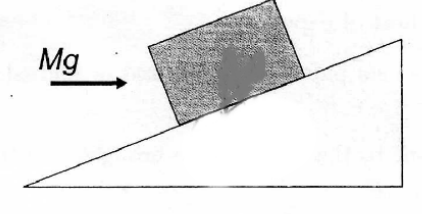
\includegraphics[width=0.5 \linewidth]{spho_book_TYS_images/2010q2.png}
\caption{Horizontal force on a block.} \label{2010q2}
\end{figure}

\subsection{Solution 2}
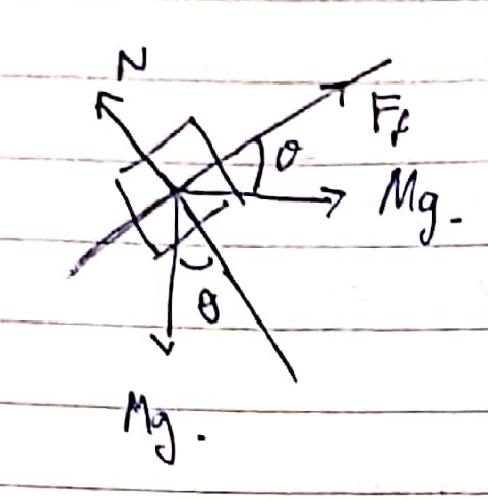
\includegraphics[width=0.3\linewidth]{spho_book_TYS_images/2010q2_2.png} \\
(i) I don't think it's possible to express $N, F_f$ purely in terms of $M,\mu$. It will depend on angle $\theta$ as well.
Balancing forces parallel to the slope, \[M_{g} \cos \theta+{I}_{f}-m g \sin \theta=0\]
Balancing forces perpendicular to the slope, \[N=M g(\sin \theta+\cos \theta)\]
Lastly, the frictional force satisfies the inequality \[\left|F_{f}\right| \leq \mu N\]
Now we just need to solve this to get \[F_{g}=-M_{g}(\sin \theta-\cos \theta)\]
and \[N=M_{g}(\sin \theta+\cos \theta)\]

(ii)
\begin{equation}
	\frac{F_{f}}{N}=\frac{\sin \theta-\cos \theta}{\sin \theta + \cos\theta}=\frac{\tan \theta-1}{\tan \theta+1}
\end{equation}
From the inequality on friction, 
\[-\mu \leq \frac{\tan \theta-1}{\tan \theta+1} \leq \mu\]
The left inequality gives
\begin{equation}
	\begin{aligned}
		&-\mu \tan \theta-\mu \leq \tan \theta-1 . \\
		& 1-\mu \leq \tan \theta(\mu+1) \\
		& \frac{1-\mu}{1+\mu} \leq \operatorname{tan} \theta
	\end{aligned}
\end{equation}
while the right one gives
\begin{equation}
	\begin{aligned}
		&\tan \theta-1 \leq \mu \tan \theta+\mu . \\
		&\tan \theta(1-\mu) \leq 1+\mu . \\
		&\tan \leq \frac{1+\mu}{1-\mu}
	\end{aligned}
\end{equation}

Hence,
\begin{equation}
	\frac{1-\mu}{1+\mu} \leq \tan \theta \leq \frac{1+\mu}{1-\mu}
\end{equation}

\subsection{Question 3}
3. A mobile is formed by supporting four metal butterflies of equal mass $m$ from a string of length $L$. The points of support are evenly spaced a distance $\ell$ apart as shown in Figure \ref{2010q3}. The string forms an angle $\theta_{1}$ with the ceiling at each end point. The center section of string is horizontal. \\
(i) Find the tension in each section of string in terms of $\theta_{1}, m$, and $g$. \\
(ii) Find the angle $\theta_{2}$, in terms of $\theta_{1}$. \\
(iii) Show that the distance $D$ between the end points of the string is
$$
D=\frac{L}{5}\left(a \cos \theta_{1}+b \cos \left[\tan ^{-1}\left(\frac{1}{2} \tan \theta_{1}\right)\right]+1\right)
$$
where $a$ and $b$ are constants to be determined. State the values of $a$ and $b$. [3] \\

\begin{figure}
\centering
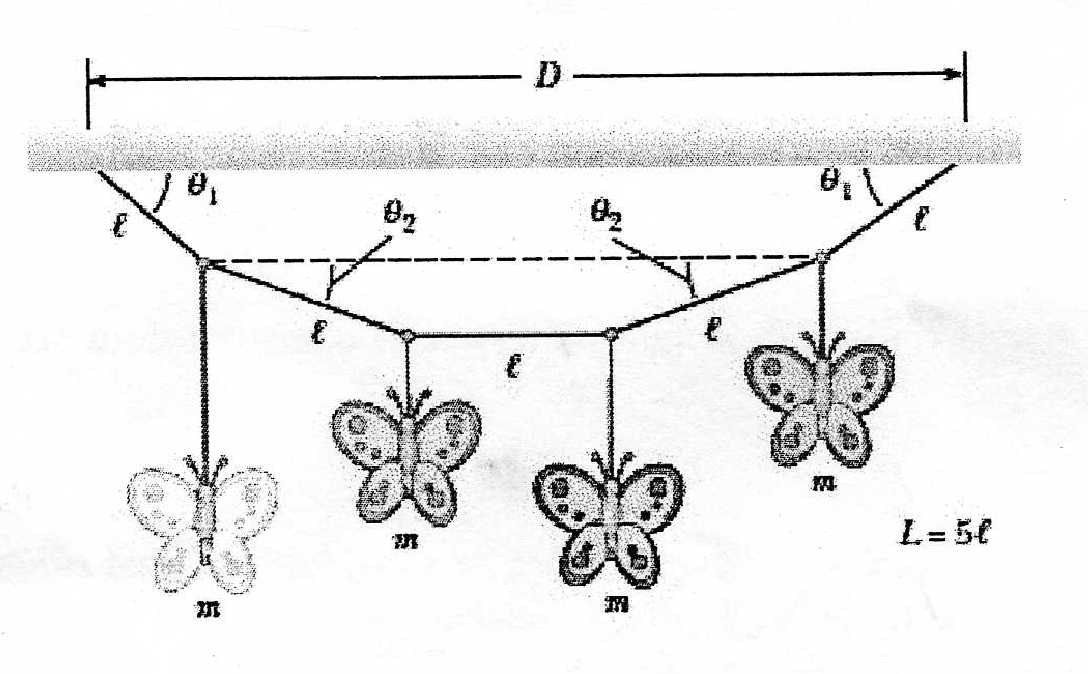
\includegraphics[width=\linewidth]{spho_book_TYS_images/2010q3.png}
\caption{A mobile is formed by supporting four metal butterflies of equal mass $m$.} \label{2010q3}
\end{figure}

\subsection{Solution 3}
For the first mass (from the left),
\begin{figure}
	\centering
	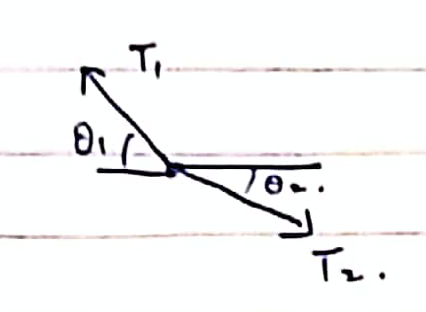
\includegraphics[width=0.5\linewidth]{spho_book_TYS_images/2010q3_2.png}
	\caption{Force body diagram of first mass from the left}
\end{figure}

balancing horizontal and vertical forces,
\[T_{1} \cos \theta_{1}=T_{2} \cos \theta_{2} \]
\[T_{1} ma_{1}=T_{2} \sin\theta_{2}+mg\]
For the second mass (from the left), balancing horizontal and vertical forces,

\begin{align}
	T_{2} \sin \theta_{2}=m g \\
	T_{3}=T_{2} \text { cos } \theta_{2}
\end{align}
The 2nd and 3rd equation lets us express $T_1$ as 
\begin{equation}
	T_{1}=\frac{2 m{g}}{\sin \theta_{1}}
\end{equation}
Then $T_3$ can be expressed as
\begin{align}
	T_{3}=T_{2} \text { cos } \theta_{2}  = T_{1} \cos \theta_{1} \\
	T_3 = \frac{2 m{g}}{\sin \theta_{1}} \cos \theta_{1}=\frac{2 m g}{\tan \theta_1}
\end{align}
Finally $T_2$ is given by
\begin{equation}
	\begin{array}{l}
		T_{2} \sin \theta_{2}=m g \\
		T_{2} \cos \theta_{2}=\frac{2 m g}{\tan \theta_{1}}=2 m g \cot \theta_{1} \\
		\Rightarrow T_{2}=m g \sqrt{1+4 \cot ^{2} \theta_{1}}
	\end{array}
\end{equation}
(ii)
\begin{equation}
	\begin{aligned}
		&\sin \theta_{2}=\frac{m g}{T_{2}} \\
		&\operatorname{sin}\theta_{2}=\frac{1}{\sqrt{1+4 \cot ^{2} \theta_{1}}} \\
		&\theta_{2}=\tan ^{-1}\left(\frac{1}{2 \cos \theta_{1}}\right) \\
		&\theta_{2}=\tan ^{-1}\left(\frac{1}{2} \tan \theta_{1}\right)
	\end{aligned}
\end{equation}
\begin{figure}
	\centering
	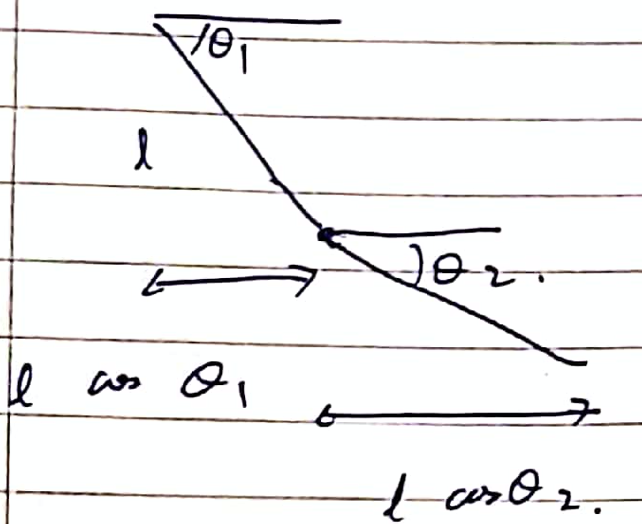
\includegraphics[width=0.5\linewidth]{spho_book_TYS_images/2010q3_3.png}
	\caption{Force body diagram of second mass from the left}
\end{figure}
Since 
\begin{equation}
	l\cos \theta_{2} =l\left(\frac{2\cos\theta_{1}}{\sqrt{1+4\operatorname{cot}^{2} \theta_{1}}}\right)
\end{equation}
Hence
\begin{equation}
	\begin{aligned}
		D &=2 l \cos \theta_{1}+2 l \cos \theta_{2}+l \\
		&=\frac{L}{5}\left(2 \cos \theta_{1}+2 \cos \left(\tan ^{-1}\left(\frac{1}{2} \tan \theta_{1}\right)\right)+1\right) \\
		& a=2, \quad b=2
	\end{aligned}
\end{equation}


\subsection{Question 4}
4. A $670 \mathrm{~kg}$ meteorite is composed of aluminum. At a distance far from the Earth, its temperature is $-15^{\circ} \mathrm{C}$ and it moves with a speed of $14.0 \mathrm{ kms}^{-1}$ relative to the Earth. As it crashes into the planet, the resulting additional internal energy is shared equally between the meteor and the planet. Assuming that all of the material of the meteor rises momentarily to the same final temperature, determine this temperature. You may also assume that the specific heat of liquid and of gaseous aluminum is 1170 $\mathrm{Jkg}^{-1} \mathrm{~K}^{-1}$, the latent heat of fusion and vaporization of aluminum are $3.97 \times 10^{5} \mathrm{~J}$ $\mathrm{kg}^{-1}$ and $1.14 \times 10^{7} \mathrm{~J} \mathrm{~kg}^{-1}$ respectvely, and the melting point and boiling point of aluminum are $660 \mathrm{~K}$ and $2450 \mathrm{~K}$ respectively.
[10]

\subsection{Solution 4}
Because $M_E >> \text{Mass of asteroid}$, earth barely changes its velocity, so half (the internal energy is shared equally between the meteor and the planet) of the meteorites kinetic energy (KE) and gravitational potential energy (GPE) is converted to heat.
\begin{equation}
	\begin{aligned}
		&E_{KE} + E_{GPE} \\
		&=\frac{1}{2}(670)\left(14.0 \times 10^{3}\right)^{2} + \frac{(6.67\times 10^{-11}) (5.97219\times10^24) (670)}{6.371 \times 10^6} \\
		&=1.075516 \times 10^{11} \mathrm{~J} \\
		&E_{converted} \\
		&=\frac{1}{2} (E_{KE} + E_{GPE}) \\
		&=5.37757 \times 10^{10} \mathrm{~J}
	\end{aligned}
\end{equation}
\begin{figure}
	\centering
	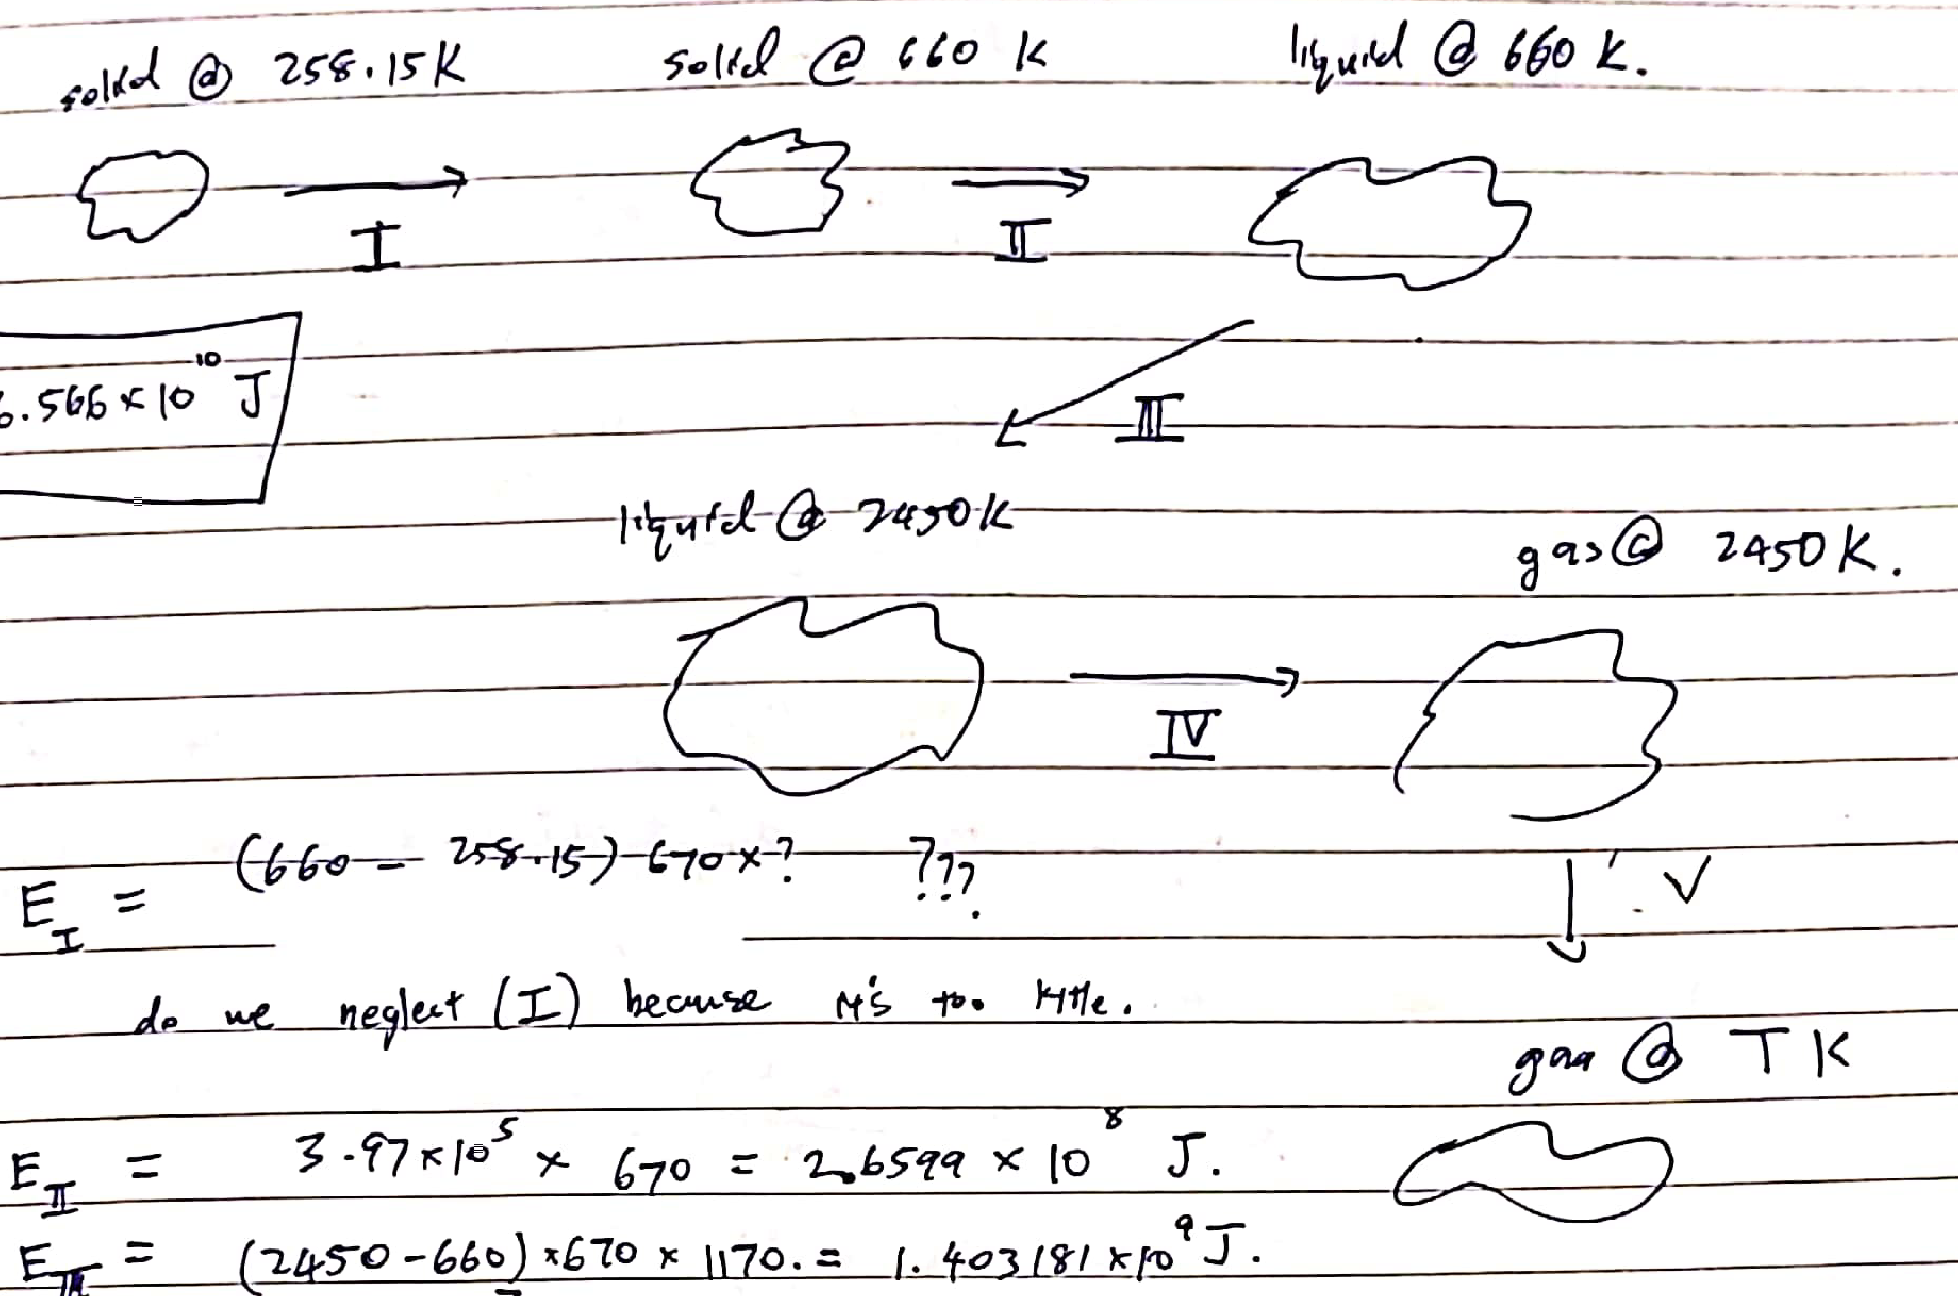
\includegraphics[width=0.9\linewidth]{spho_book_TYS_images/2010q4.png}
	\caption{Phase transitions, please ignore my working on the bottom left.}
\end{figure}
We don't know the heat capacity for solid aluminium, so I am just assuming we don't need to account for process (I). A quick google search tells us that it is $900 \mathrm{~J} / \mathrm{kg}^{\circ} \mathrm{C}$ which means $E_{I} = (660-258.15) \times 670 \times 900 = 2.4232 \times 10^{8} \mathrm{~J}$, which is small compared to $E_{II}+...+E_{IV}=9.3072 \times 10^9 \mathrm{~J}$ anyway. I would accept both answers personally since this question involves so much approximation anyway.
\begin{equation}
	\begin{aligned}
		&E_{II}=3.97 \times 10^{5} \times 670=2.6599 \times 10^{8} \mathrm{~J} .\\
		&E_{III}=(2450-660) \times 670 \times 1170 =1.403181 \times 10^{9} \mathrm{~J} .\\
		&E_{IV}=1.14 \times 10^{7} \times 670=7.638 \times 10^{9} \mathrm{~J}\\
		&E_{V}=5.37757 \times 10^{10}-E_{II}-E_{III}-E_{IV}\\
		&=4.4469 \times 10^{10} \mathrm{~J}
	\end{aligned}
\end{equation}
The remaining energy goes into heating the gas,
\begin{equation}
	\begin{aligned}
		T - {2450}&=E_{V} / (670 \times 1170) =56727 \mathrm{~K} \\
		T &= 59177 \mathrm{~K} \text {(so high :O??)}
	\end{aligned}
\end{equation}

\subsection{Question 5}
5. A pion at rest with a mass $m_{\pi}$ decays to a muon of mass $m_{\mu}$ and an antineutrino of negligible mass. The reaction is written as $\pi^{-} \rightarrow \mu^{-}+\bar{\nu}$. Calculate the kinetic energy of the muon and the energy of the antineutrino in electron volts. You may take $m_{\pi}=273 m_{e}$ and $m_{\mu}=207 m_{e}$ where $m_{e}$ is the rest mass of the electron.
$[9]$
\subsection{Solution 5}
Before the collision,
\begin{equation}
	\begin{aligned}
		E_{\pi}^{2} &=m_{\pi}^{2} \\
		E_{\pi} &=m_{\pi} \\
		E_{\mu}+E_{\nu} &=E_{\pi}
	\end{aligned}
\end{equation}
\begin{equation}
	\begin{aligned}
		&E_{\mu}^{2}-p_{\mu}^{2}=m_{\mu}{ }^{2}\\
		&E_{V}^{2}-p_{\nu}^{2}=m_{\nu}^{2}\\
		&p_{\mu}=-p_\nu\\
		&E_{\mu}^{2}-E_{V}^{2}=m_{\mu}{ }^{2}-m_{\nu}{ }^{2}\\
		&\left(E_{\mu}+E_{\nu}\right)\left(E_{\mu}-{E_\nu}\right)=m_{\mu}^{2}-m_{\nu}{ }^{2}\\
	\end{aligned}
\end{equation}
\begin{equation}
	\begin{aligned}
		&E_{\mu}-E_{\nu}=\frac{m_{\mu}^{2}-m_{\nu}^2}{m_{\pi}} \\
		&E_{\mu}+E_{\nu}=m_{\pi} \\
		&E_{\mu}=\frac{1}{2}\left(m_{\pi}+\frac{m_{\mu}^{2}-m_{\nu}^2}{m_{\pi}}\right)= \frac{1}{2}\left(m_{\pi}+m_{\mu}^{2} / m_{\pi}\right) \\
		&E_{V}=\frac{1}{2}\left(m_{\pi}-\frac{m_{1}^{2}-m_{\nu}^{2}}{m_{\pi}}\right)=\frac{1}{2}\left(m_{\pi}-m_{\mu}^{2} / m_{\pi}\right)
\end{aligned}
\end{equation}
Putting units back to obtain numerical values,
\begin{equation}
	\begin{aligned}
		&E_{\mu}=\frac{1}{2}\left(\frac{m_{\pi}^{2}+m_{\mu}^{2}}{m_{\pi}}\right) c^{2} \\
		&E_{\nu}=\frac{1}{2}\left(\frac{m_{\pi}^{2}-m_{\mu}^{2}}{m_{\pi}}\right)c^{2}
	\end{aligned}
\end{equation}
This gives us 
\begin{align}
	E_\mu &= 1.7590 \times 10^{-11} \text{ J}\\
	E_\nu &= 4.7474 \times 10^{-11} \text{ J}
\end{align}

\subsection{Question 6}
6. A smaller disk of radius $r$ and mass $m$ is attached rigidly to the face of a second larger disk of radius $R$ and mass $M$ as shown in Figure \ref{2010q6}. The center of the small disk is located at the edge of the large disk. The large disk is mounted at its center on a frictionless axle. The assembly is rotated through a small angle $\theta$ from its equilibrium position and released. \\
(i) Show that the speed of the center of the small disk as it passes through the equilibrium position is
$$
v=\alpha\left[\frac{R g(1-\cos \theta)}{(M / m)+(r / R)^{2}+\beta}\right]^{1 / 2}
$$
where $\alpha$ and $\beta$ are constants to be determined. State the values of these constants. [7]\\
(ii) Determine the period of the motion in terms of $M, m, R$ and $r$. [3]
\begin{figure}
	\centering
	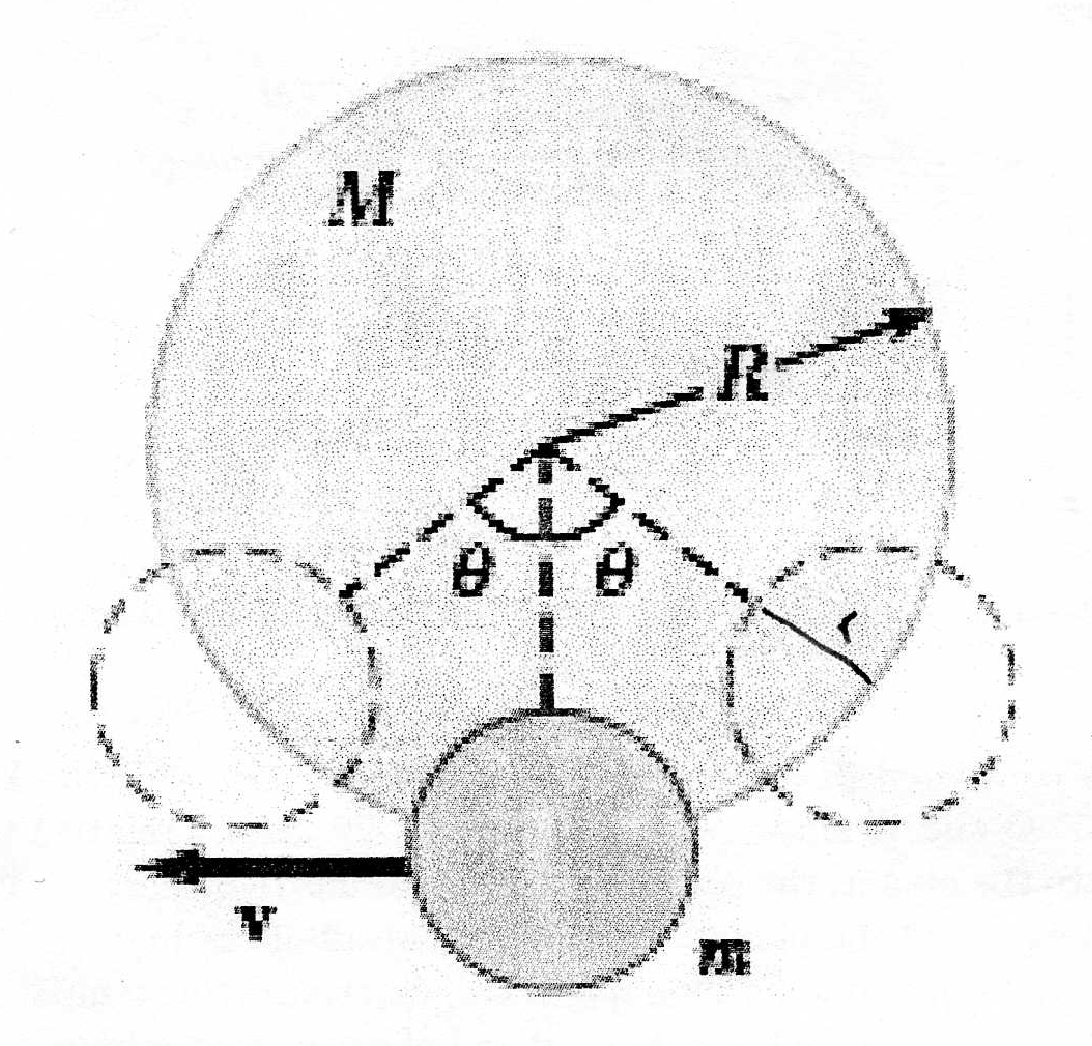
\includegraphics[width=0.5\linewidth]{spho_book_TYS_images/2010q6.png}
	\caption{A smaller disk of radius $r$ and mass $m$ is attached rigidly to the face of a second larger disk of radius $R$ and mass $M$}\label{2010q6}
\end{figure}

\subsection{Solution 6}
(i)
\begin{equation}
	\begin{aligned}
		&\omega=\frac{v}{R}\\
		&\frac{1}{2}I_{1} \omega^{2}+\frac{1}{2} m v^{2}+\frac{1}{2} I_{2} \omega^{2}=m g R(1-\cos \theta)\\
		&\frac{1}{2} \frac{1}{2} M R^{2} \frac{v^{2}}{R^{2}}+\frac{1}{2} m v^{2}+\frac{1}{2} \frac{1}{2} \operatorname{mr}^{2} \frac{v^{2}}{R^{2}}=mgR(1-\cos \theta)\\
		&v^{2}\left(\frac{1}{4} M+\frac{1}{2} m+\frac{1}{4} m \frac{r^{2}}{R^{2}}\right)=m g R(1-\cos \theta)\\
		&v^{2}=\frac{g R(-1-\cos \theta)}{\frac{1}{4}\frac{M}{m}+\frac{1}{4}\left(\frac{r}{k}\right)^{2}+\frac{1}{2}}\\
		&=4 \frac{g R(1-\cos \theta)}{\frac{M}{m}+\left(\frac{r}{R}\right)^{2}+2}\\
		&V=2 \sqrt{\frac{{g r(1-\cos \theta)}}{\frac{M}{n}+\left(\frac{r}{R}\right)^{2}+2}}\\
		&\alpha=2, \quad \beta=2
	\end{aligned}
\end{equation}
(ii) 
$\frac{1}{2} I_{1} \omega^{2}+\frac{1}{2} m^{2}+\frac{1}{2} I_{2} \omega^{2}+m g R(1-\cos \theta)=\text{const}$ \\
$\dot{\theta}^{2}\left(-\frac{1}{4} m R^{2}+\frac{1}{2} m^{2}+\frac{1}{4} m r^{2}\right)=m g(\cos \theta-1)+\text{const}\approx m g R\left(-\frac{\theta^{2}}{2}\right)+$ const. \\
Differentiating wrt $\theta$,
$$
\begin{aligned}
	&2 \ddot{\theta} \alpha=\operatorname{mgR} \theta=\theta . \\
	&\ddot{\theta}+\frac{m g R}{\frac{1}{2} m R^{2}+m R^{2}+\frac{1}{2} m r^{2}} \theta=0 .
\end{aligned}
$$
$$
\omega=\sqrt{\frac{2 m g R}{M R^{2}+2 {M R}^{2}+m r^{2}}}
$$
\begin{equation}
	T=\frac{2 \pi}{\omega}=2 \pi \sqrt{\frac{M R^{2}+2 m R^{2}+m r^{2}}{2 m g}}
\end{equation}
\subsection{Question 7}
7. An electric motor turns a flywheel through a drive belt that joins a pulley on the motor and a pulley that is rigidly attached to the flywheel, as shown in Figure \ref{2010q7}. The flywheel is a solid disk with a mass of $80.0 \mathrm{~kg}$ and a diameter of $1.25 \mathrm{~m}$. It turns on a frictionless axle. Its pulley has a much smaller mass and a radius of $0.230 \mathrm{~m}$. If the tension in the upper (taut) segment of the belt is $135 \mathrm{~N}$ and the flywheel has a clockwise angular acceleration of $1.67 \mathrm{rads}^{-2}$, find the tension in the lower (slack) segment of the belt.
$[4]$

\begin{figure}
	\centering
	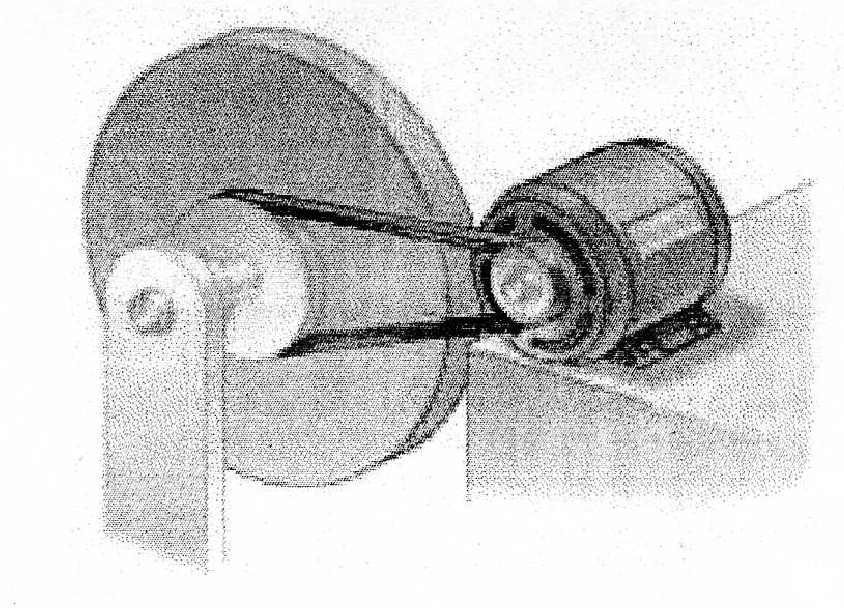
\includegraphics[width=0.5\linewidth]{spho_book_TYS_images/2010q7.png}
	\caption{An electric motor turns a flywheel through a drive belt that joins a pulley on}\label{2010q7}
\end{figure}
\subsection{Solution 7}
$\begin{aligned}
	&I{\alpha}=(\Delta T) r\\
	&\Delta T=\frac{\frac{1}{2} m R^{2} \alpha}{r} \\
	&=\frac{\frac{1}{2}(80)\left(\frac{1.25}{2}\right)^2 (1.67)}{0.230}\\
	&=113.45\\
	&\text {Bottom tension}=135-\Delta T\\
	&=21.55 \mathrm{~N} 
\end{aligned}$

\subsection{Question 8}
8. A plano-concave lens having index of refraction $1.50$ is placed on a flat glass plate, as shown in Figure \ref{2010q8}. Its curved surface, with radius of curvature $8.00 \mathrm{~m}$, is on the bottom. The lens is illuminated from above with yellow sodium light of wavelength $589 \mathrm{~nm}$, and a series of concentric bright and dark rings is observed by reflection. The interference pattern has a dark spot at the center, surrounded by 50 dark rings, of which the largest is at the outer edge of the lens. \\
(i) What is the thickness of the air layer at the center of the interference pattern? \\
(ii) Calculate the radius of the outermost dark ring. \\
(iii) Find the focal length of the lens. [9]

\begin{figure}
	\centering
	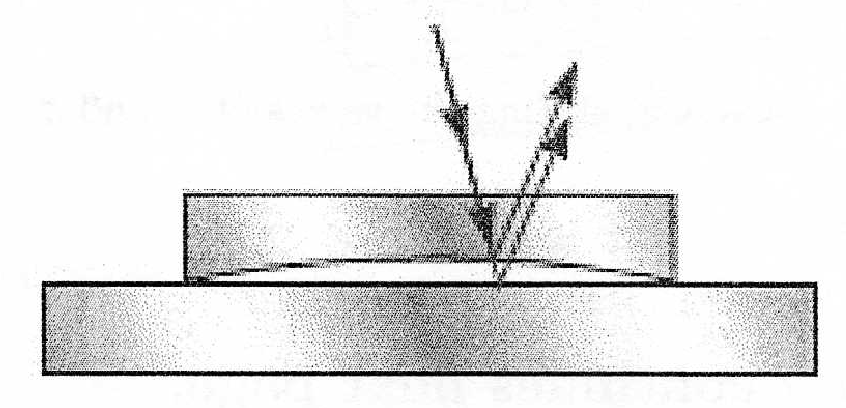
\includegraphics[width=0.5\linewidth]{spho_book_TYS_images/2010q8.png}
	\caption{A plano-concave lens placed on a flat glass plate} \label{2010q8}
\end{figure}
\subsection{Solution 8}
Remember that reflection has a $\pi$ phase shift. Neglect refraction effects. The optical path difference is responsible for interference.
(i) 
$$\begin{aligned}
	&2 d=51 \lambda \\
	&d=\frac{51}{2} \lambda=1.502 \times 10^{-5} \mathrm{~m} .
\end{aligned}$$
(ii) 
$$
\begin{aligned}
	& \sqrt{8^{2}-(8-d)^{2}} \\
	=& 0.0155 \mathrm{~m}\quad \text{(3sf)} \\
	=& 1.55 \text{ cm} \\
\end{aligned}
$$
(iii)
$$\begin{aligned}
	&\frac{1}{f}=(1.5-1)\left(\frac{1}{-8}\right) \\
	&\frac{1}{1}=-0.0625 \\
	&f=-16 \text{ m}
\end{aligned}$$


\subsection{Question 9}
9. (a) A toroid has a major radius $R$ and a minor radius $r$ and it is tightly wound with $N$ turns of wire, as shown in Figure \ref{2010q9}. If $R>>r$, the magnetic field in the region enclosed by the wire of the torus, of cross-sectional area $A=\pi r^{2}$, is essentially the same as the magnetic field of a solenoid that has been bent into a large circle of radius $R$.\\
\begin{figure}
	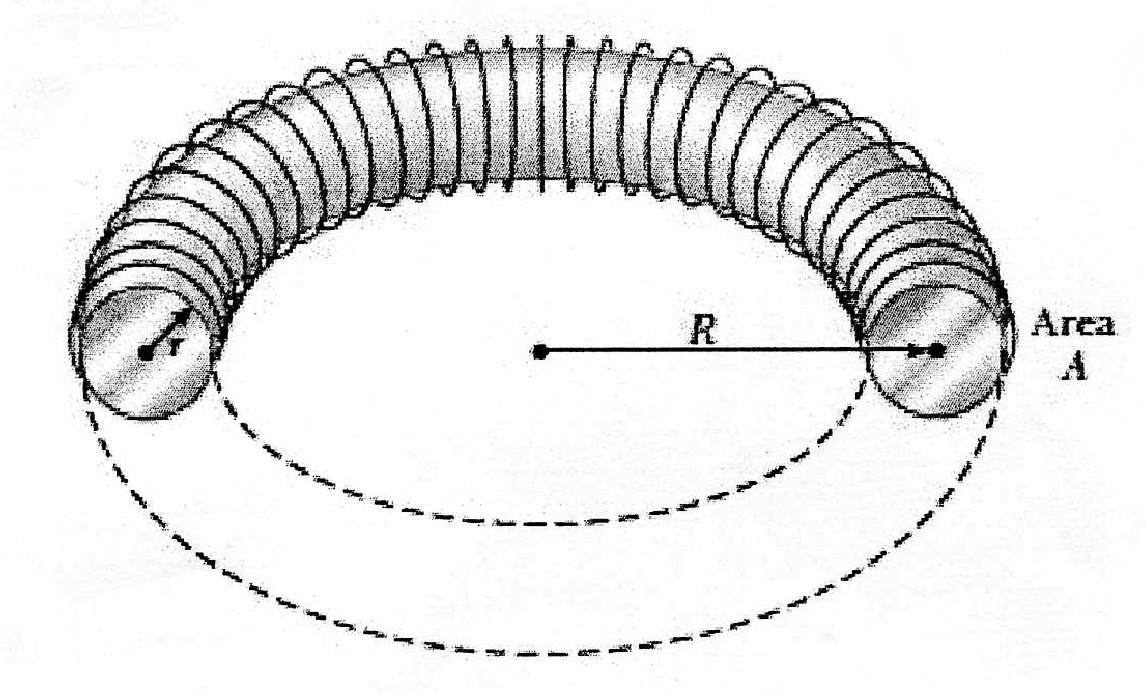
\includegraphics[width=0.8\linewidth]{spho_book_TYS_images/2010q9.png}
	\caption{A toroid has a major radius $R$ and a minor radius $r$ and it is tightly wound with $N$ turns of wire.} \label{2010q9}
\end{figure}
Show that the self-inductance of such a toroid is approximately
$$
L \approx \kappa \mu_{0} \frac{N^{\alpha} A}{R}
$$
where $\kappa$ and $\alpha$ are constants. State the values of $\kappa$ and $\alpha$.
(b) The toroid in Figure \ref{2010q9} with $N$ turns of wire is now replaced by one with a rectangular cross section. Its inner and outer radii are $a$ and $b$, respectively. The cross-section is a rectangle of length $b-a$ and breadth $h$.
(i) Show that the inductance of the toroid is
$$
L=\kappa^{\prime} \mu_{0} \frac{N^{\beta} h}{R} \ln \frac{b}{a}
$$
where $\kappa^{\prime}$ and $\beta$ are constants, stating the values of $\kappa^{\prime}$ and $\beta$ [4]. \\
(ii) Compute the self-inductance of a 500-turn toroid for which $a=10.0 \mathrm{~cm}$, $b=12.0 \mathrm{~cm}$, and $h=1.00 \mathrm{~cm}$. In part (a), an approximate expression for the inductances of a toroid with $R>>r$ was derived. If the calculations in part (b) (ii) were done using this approximate expression for self-inductance, what is the percentage error in the result? \\
\begin{figure}
	\centering
	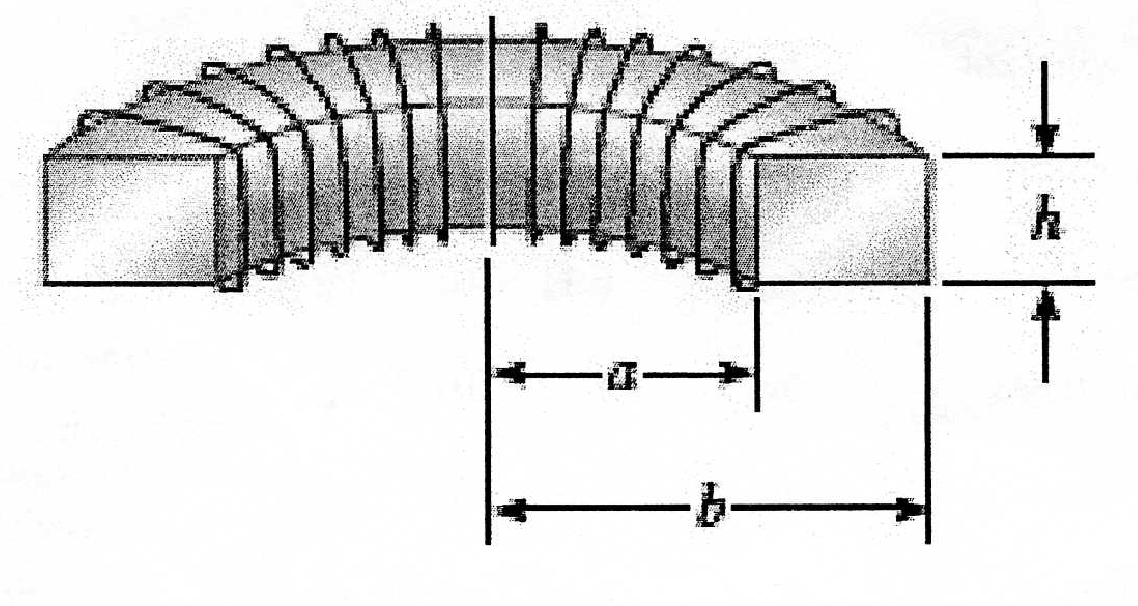
\includegraphics[width=0.8\linewidth]{spho_book_TYS_images/2010q9_2.png}
	\caption{A toroid with a rectangular cross-section.} \label{2010q9_2}
\end{figure}
\subsection{Solution 9}
(a) 
$$N \Phi=L I .$$
$$\overbrace{\frac{\mu N I}{2 \pi R}}^{B} A N=L I$$
$$L=\frac{1}{2 \pi} \frac{\mu_{0}  N^{2} A}{R}$$
$$\kappa=\frac{1}{2 \pi}, \quad \alpha=2$$
(b) (i)
$$2 \pi x B=\mu N I$$
$$B=\mu N I / 2 \pi x$$
$$\Phi=h \int_{a}^{b} B d x=\mu \frac{h N I}{2 \pi} \ln \frac{b}{a} .$$
$$L=\frac{\Phi N}{I}=\mu \frac{h N^{2}}{2 \pi} \ln \frac{b}{a} .$$
$$L=\frac{R}{2 \pi} \mu_{0} \frac{N^{2} h}{R} \ln \frac{b}{a}$$
$$k^{\prime}=\frac{R}{2 \pi}$$
$$\beta=2$$
(ii) 
\begin{align}
	L_{\text{circular}} &= \frac{1}{2\pi} \mu_0 \frac{N^2 A}{R}\\
	&=9.09 \times 10^{-5} \mathrm{H} \quad \text{(3 sf)}\\
	L_{\text {exact }}&=\frac{1}{2 \pi} \mu_{0} \cdot N^{2} h\ln \frac{b}{a}\\
	&=9.12 \times 10^{-5} \mathrm{H} \quad \text{(3 sf)}
\end{align}
\% error $= \frac{L_{exact}-L_{circular}}{L_{exact}} = 0.286\% \quad \text{(3sf)}$.

\subsection{Question 10}
10. An empty box of total mass $M$ with perfectly reflecting walls is at rest in the lab frame. Then electromagnetic standing waves are introduced along the $x$ direction, consisting of $N$ photons, each of frequency $\nu$ as shown in Fig. 8. Determine the rest mass of the system (box + photons) when the photons are present.
\begin{figure}
	\centering
	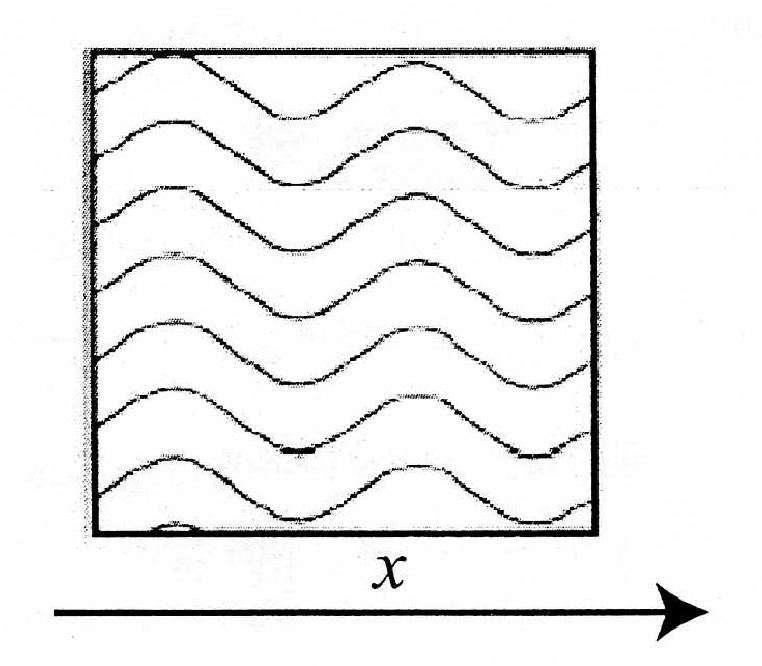
\includegraphics[width=0.5\linewidth]{spho_book_TYS_images/2010q10.png}
	\caption{An empty box of total mass $M$ with perfectly reflecting walls is at rest in the lab frame.}
\end{figure}
\subsection{Solution 10}
I don't know.

\section{2011}

\subsection{Question 1}
1. A pendulum consists of a copper sphere of radius $R$ and density $\varrho$ suspended from a string. Due to the drag from the air the amplitude of the oscillation $A$ decays with time $t$ as
$$
A=A_{0} \exp (-\gamma t)
$$
where $\gamma=\frac{9 \eta}{4 R^{2} \varrho}$. Ao is the initial amplitude of the pendulum and $\eta$ is the viscosity of air. The measurement of the amplitudes is accurate to $1\%$ with other measurement provided below
$$
\begin{aligned}
	&\eta=(1.78 \pm 0.02) \times 10^{-5} \mathrm{~kg} \mathrm{~m}^{-1} \mathrm{s}^{-1} \\
	&R=5.2 \pm 0.2 \mathrm{~mm} \\
	&\varrho=(0.89 \pm 0.05) \times 10^{3} \mathrm{~kg} \mathrm{~m}^{-3}
\end{aligned}
$$
Evaluate the time taken for the amplitude to fall to $85 \%$ of the initial amplitude $A_{0}$ and the error in this quantity. State the parameter that contributes the biggest error to the final result [8]

\subsection{Solution 1}
\[A=A_0 \exp{(-\gamma t)}\]
Solve for $t$ when $A_0\exp{(-\gamma t)} = 0.85 A_0$
\begin{align}
	t &= -\frac{1}{\gamma} \ln{0.85} \\
	&= -\frac{4R^2\varrho}{9\eta} \ln{0.85} \\
	&= 97.656\text{s}
\end{align}
To find the uncertainty,
\[\frac{\Delta t}{t} = 2\frac{\Delta R}{R} + \frac{\Delta \varrho}{\varrho} + \frac{\Delta \eta}{\eta} + \frac{\Delta \left(\ln\frac{A}{A_0} \right)}{\left|\ln{\frac{A}{A_0}}\right|}\]
To find $\Delta \left(\ln{\frac{A}{A_0}}\right)$ (remembering there is uncertainty in the measurement of $A$ and $A_0$ too),
\begin{align}
	\Delta\left(\ln{\frac{A}{A_0}}\right) &= \Delta(\ln{A} -\ln{A_0}) \\
	&= \frac{\Delta A}{A} + \frac{\Delta A_0}{A_0}
\end{align}
where $\frac{\Delta A}{A} = \frac{\Delta A_0}{A_0} = 0.01$ is given in the question
\begin{align}
	\frac{\Delta R}{R} &= \frac{0.2}{5.2} \\
	\frac{\Delta \varrho}{\varrho} &= \frac{0.05}{0.89} \\
	\frac{\Delta \eta}{\eta} &= \frac{0.02}{1.78} \\
	\frac{\Delta \left(\ln\frac{A}{A_0} \right)}{\left|\ln{\frac{A}{A_0}}\right|} &= \frac{0.01 + 0.01}{ \left| \ln{0.85} \right| }\\
	&= 0.26740 \\
	\Delta t &= 0.26740 \times 97.565 \\
	&= 26 \text{ s (nearest second)} \\
	t &= (98 \pm 26) \text{ s}
\end{align}
Comments: \\
In olympiad it mostly suffices to use the rule \[\Delta f(x_1,x_2,...,x_n) = \left|\frac{\partial f}{\partial x_1}\right| \Delta x_1 + \left|\frac{\partial f}{\partial x_2}\right| \Delta x_2 +...+ \left|\frac{\partial f}{\partial x_n}\right| \Delta x_n \] that looks similar to the multivariate calculus chain rule \[df = \sum_i \frac{\partial f}{\partial x_i} dx_i\]
For example, if $f(a,b,c) = a^2b + c$,
\begin{align}
	\Delta f &= \left| \frac{\partial f}{\partial a} \right| \Delta a + \left| \frac{\partial f}{\partial b} \right| \Delta b + \left| \frac{\partial f }{\partial c} \right| \Delta c  \\
	&= |2ab| \Delta a + |a^2| \Delta b + \Delta c \\
	&= \Delta(a^2 b) + \Delta c\\
	\text{where } \frac{\Delta(a^2 b)}{|a^2 b|} &= \frac{2\Delta a}{|a|} + \frac{\Delta b}{|b|}
\end{align}
The (olympiad) set of rules are then
\begin{align}
	\Delta(A+B) &= \Delta A + \Delta B \\
	\Delta(A-B) &= \Delta A + \Delta B \\
	\frac{\Delta (A\times B)}{|A\times B|} &= \frac{\Delta A}{|A|} + \frac{\Delta B}{|B|} \\
	\frac{\Delta (A\div B)}{|A\div B|} &= \frac{\Delta A}{|A|} + \frac{\Delta B}{|B|}
\end{align}
But in reality, there isn't a hard rule for the calculation of errors and uncertainty. The proper way to do so is using statistics (\url{https://en.wikipedia.org/wiki/Propagation_of_uncertainty}), in which uncertainty is the standard deviation of the distribution of measurements. One commonly used formula is the "quadrature uncertainty".

\subsection{Question 2}
2. In this question you are asked to make reasoned estimates and assumptions. These must be clearly stated.
(a) Figure 1 shows an equilateral glass prism illuminated by a 100 W laser beam of wavelength $\lambda=600$ nm. The refractive index of the glass of the prism is $1.50$ at $\lambda=600 \mathrm{~nm}$. The path of the light in the prism is parelel to the base of the prism. Calculate the change in weight of the prism when the beam is switched on. [4]
\begin{figure}
	\centering
	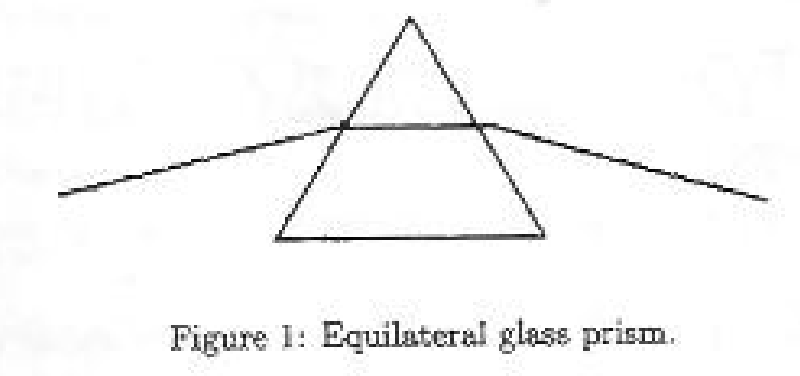
\includegraphics[width=0.8\linewidth]{spho_book_TYS_images/2011q2.png}
	\caption{Equilateral glass prism}
\end{figure}
(b) Optical treezers, which are composed of two lasers beams, are able to manipulate small transparent spheres. Explain clearly how this can be done and why at least two beams are needed. [3]
(c) Small smoke particles in air are seen under a low magnificaton microscope to move randomly at speed of $0.10 \mathrm{~mm}^{-1}$. The speed of sound in air is $20 \mathrm{~m} \mathrm{~s}^{-1}$. Estimate the mass of the smoke particles. [3]

\subsection{Solution 2}
(a) First, find $\theta_i$ by using Snell's law.
\begin{align}
	\sin \theta_i &= 1.5 \sin \theta_r = 0.75 \\
	\theta_i &= 48.590^\circ
\end{align}
Then consider the momentum of one photon before entering the glass and after exiting the glass
\[\Delta p_{vert} = 2p_{photon} \sin{(\theta_i - 30^\circ)} = 2p_{photon} \sin{18.590^\circ}\]
The momentum of a photon is given by the De Broglie wavelength relation (Quantum Mechanics) $p_{photon} = \frac{h}{\lambda}$ where $h$ is Planck's constant and $\lambda$ is the wavelength of the photon. How many photons hit the glass in 1 second?
\[\text{Power} = \frac{\text{Energy}}{\text{Time}} = \frac{hc}{\lambda} \times \frac{\text{No. photons}}{\text{Time}} \]
where $\frac{hc}{\lambda}$ is the energy of one photon. Without explicitly calculating $\frac{h}{\lambda}$, we can now write the force in terms of the power.
\begin{align}
	\text{Force} &= \frac{\Delta p_{vert}}{\text{Time}} \times \text{No. photons} \\
	&= 2\times \frac{\text{Power}}{c} \times \sin(18.590^\circ) \\
	\text{Force} &= 2.1253\times 10^{-7} \text{ N}
\end{align}
Comments:\\
For photon pressure questions, dimensional analysis tends to be useful in guiding your conceptual understanding and checking your formulas.\\
The relativistic energy relation $E^2 = m^2 c^4 + p^2 c^2$ applies to photons as well, where the momentum of a photon is given by the De Broglie relation $\lambda = h/p$\\
For further reading, check out "radiation pressure" and "poynting vector".\\
(b) TODO\\
(c) The speed of sound in a gas is given by \[c=\sqrt{\frac{\gamma P_0}{\rho}}\] where $\gamma$ is the adiabatic constant, $P_0$ is the pressure of the gas, $\rho$ is the density of the gas.
Assuming air to be an ideal gas, $P_0 V = nRT\rightarrow P_0 = \frac{M}{\mu} \frac{RT}{V} = \frac{RT}{\mu} \rho$ where $M$ is the total mass of the gas and $\mu$ is the mass of 1 mole of gas.
Hence, $c=\sqrt{\frac{\gamma RT}{\mu}} $ is the speed of sound.
The speed of sound is related (but not equal!) to the RMS speed $v_{rms}$.
\begin{align}
	\frac{1}{2} n \mu v_{rms}^2 &= \frac{3}{2} nRT\\
	v_{rms} &= \sqrt{\frac{3RT}{\mu}} \\
	&= \sqrt{\frac{3}{\gamma}} \sqrt{\frac{\gamma RT}{\mu}} \\
	&= \sqrt{\frac{3}{\gamma}} c
\end{align}
For air which is around 78\% $\text{N}_2$ and 21\% $\text{O}_2$, let's approximate the no. degrees of freedom to be $f=5$. This gives $\gamma = \frac{f+2}{f} = \frac{7}{5}$.
$v_{rms} = \sqrt{\frac{3}{\gamma}} c = 483.07 \text{ m s}^{-1}$.

\subsection{Question 3}
3. Suppose that we have a string of equally spaced beads of mass m such that their
surfaces are separated by a distance d. The beads are free to slide without friction
on 4 thin wire. Suppose that there is a constant force F acting on the first bead,
initially at rest, and causing it to accelerate along the wire as shown in Figure 2.
This force acts only on the first bead and might be created by a well directed, steady
stream of air. The first bead will collide with the second, which will in turn collide
with the third, and so on. Suppose that all collisions are elastic.

\begin{figure}
	\centering
	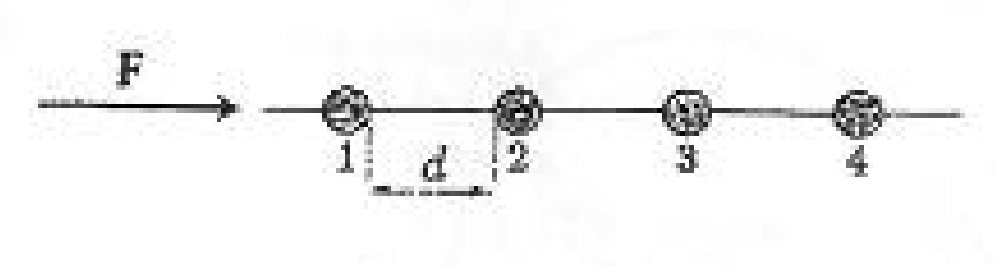
\includegraphics[width=0.7\linewidth]{spho_book_TYS_images/2011q3.png}
	\caption{Beads on wire}
\end{figure}

(i) What is the speed of the first bead immediately before and immediately after its collision with the second bead? [2] \\
(ii) What is the speed of the second bead immediately before and immediately after its collision with the third bead? [2] \\
(iii) Note that the constant force is always acting upon the first bead. What is the time interval between subsequent collisions between the first and second beads? What then is the average speed of the first bead? What is the speed of the “shock wave" that travels down the wire? [3] \\
(iv) If the whole process is repeated, but with collisions which are perfectly inelastic, what is the terminal speed of the shock wave formed? [3] \\

\subsection{Solution 3}
(i) Let the speed of the 1st bead immediately before colliding with the 2nd bead be $v_0$.
\[v_0^2 = 2ad = \frac{2Fd}{m}\]
\[v_0 = \sqrt{\frac{2Fd}{m}}\]
Right after the collision, since the 2nd bead was initially at rest, and has the same mass as the 1st bead, the 1st bead has speed 0 and 2nd bead has speed $v_0$.
(ii) Since the 1st bead does not hit the 2nd bead before the 2nd bead hits the 3rd bead (we will prove this in (iii)),
\begin{align} 
	\text{speed of 2nd bead before collision} &= v_0 \\
	\text{speed of 2nd bead after collision} &= 0
\end{align}
(iii) 
\[\frac{1}{2}\frac{F}{m} t^2 = d\] $t=\frac{2md}{F}$ is the time interval. This answers the first part of (iii). \\
We can now check that the 1st bead does not collide with the 2nd bead before the 2nd bead collides with the 3rd.
\[v_0 t = \sqrt{\frac{2Fd}{m}} \sqrt{\frac{2md}{F}} = 2d > d\]
The 2nd bead would have travelled $2d$ in the time the 1st bead travelled $d$ (to the 3rd bead's starting position). \\
The average speed is then \[v_{ave} = \frac{d}{t} = \frac{d}{\sqrt{\frac{2md}{F}}} = \frac{Fd}{2m} = \frac{1}{2} v_0\]
The speed of the shockwave is just $v_0$. You may think of the speed of the shockwave as the collissions and how they move down the chain. Each successive collission is distance $d$ apart and takes time $d/v_0$ seconds. Hence the speed is just $d/(d/v_0) = v_0$.
(iv) We solve this with various methods. \\
Method 1: \\ 
This is an exact method but it requires numerical calculation which is not available during the competition. Method 2 would be preferred during the competition.
Let $v_n$ be the velocity of the lump of mass $m$. By conservation of momentum,
Before: insert diagram
After: insert diagram
\begin{align}
	(n+1) m v_n' &= nm v_n\\
	\rightarrow	v_n' &= \frac{n}{n+1} v_n
\end{align}
The $(n+1)m$ mass then undergoes acceleration caused by force $F$ until the moment right before it collides with the $(n+2)$-th mass.
\[v_{n_1}^2 = v_n'^2 + 2 \frac{F}{(n+1)m} d = \frac{n^2}{(n+1)^2} v_n^2 + 2\frac{F}{(n+1)m} d \]
\[v_{n+1} = \sqrt{\frac{n^2 v_n^2}{(n+1)^2} + \frac{2Fd}{(n+1)m}}\]
Numerically, one can solve this recurrence relation to obtain $v_n \rightarrow \sqrt{\frac{Fd}{m}}$, which is the terminal velocity.\\
I still don't know how to solve this without resorting to numerical methods like Mathematica. However, method 2 is completely doable in a competition setting.

Method 2: \\
This method is not 100\% precise, but it replaces the discrete problem with a continuous one. \\
Let $M$ be the mass of the collected beads.
\begin{align}
	F &= \frac{d}{dt} (Mv) \\
	&= \frac{dM}{dt} v + M \frac{dv}{dt}
\end{align}
Since $\frac{dv}{dt} = 0$ at terminal velocity,
\begin{align}
	F &= \frac{dM}{dt} v \\
	&= \frac{dM}{ds} \frac{ds}{dt} v \quad \text{where } s \text{ is the displacement of the collected beads}\\
	&= \frac{m}{d} v^2 \quad \text{ since }\quad \left(\frac{dM}{ds} = \frac{m}{d}\right)\\
	v &= \sqrt{\frac{Fd}{m}}
\end{align}
And we are done!

\subsection{Question 4}
4. A zoom lens system is a combination of lenses that produces a variable magnification while maintaining fixed object and image positions. The magnification is varied by moving one or more lenses along the axis. While multiple lenses are used in practice to obtain high-quality images, the effect of zooming in on an object can be demonstrated with a simple two-lens system. An object, two converging lenses, and a screen are mounted on an optical bench. The first lens, which is to the right of the object, has a focal length of 5.0 cm, and the second lens, which is to the right of the first lens, has a focal length of 10.0 cm. The screen is to the right of the second lens. Initially, an object is situated at a distance of 7.50 cm to the left of the first lens, and the image formed on the screen has a magnification of 1.00. \\
\\
(i) Determine the distance between the object and the screen. [4] \\
(ii) Both lenses are now moved along their common axis, while the object and the screen maintain fixed positions, until the image formed on the screen has - magnification of $+3.00$. Find the displacement of each lens from its initial position in (i). [4] \\
(iii) Can the lenses be displaced in more than one way? [4] \\

\subsection{Solution 4}
(i) Concept: When looking at multiple lens systems, we simply treat the image formed by one lens as the object for the next lens. Convince yourself by considering where all possible light rays pass through after the first lens. \\
insert diagram \\
Namely, it is important to note that this approach assumes the radius of the lens is infinite. It is worth considering cases where the lens has finite radius, which will produce a "trimmed image". While these type of questions have not appeared in SPhO, they have appeared n other competitions like EuPhO 2020 Q3. \\
Anyway, returning to the question, (i) is just a direct application of this "multiple lens" concept with simple algebraic manipulation.\\
insert diagram
\[f_1 = 5.00 \text{ cm}\]
\[f_2 = 10.00 \text{ cm}\]
\[x_0 = 7.50 \text{ cm}\]
\[M = \frac{y}{x-x_1} \frac{x_1}{x_0} = 1.00\]
\[\frac{1}{x_0} + \frac{1}{x_1} = \frac{1}{f_1}\]
\[x_1 = \frac{x_0 f_1}{x_0 - f_1} = 15.0 \text{ cm}\]
\[\frac{y}{x-x_1} \frac{x_1}{x_0} = 1\]
\[y=\frac{x_0}{x_1} (x-x_1) \Rightarrow \frac{1}{y} = \frac{x_1}{x_0(x-x_1)}\]
\[\frac{1}{f_2} = \frac{1}{x-x_1} + \frac{1}{y}\]
\[ \frac{1}{f_2} = \frac{1}{x-x_1} + \frac{x_1}{x_0} \frac{1}{x-x_1} \]
\[ x - x_1 = \left(1+\frac{x_1}{x_0}\right) f_2 \]
\[x = \left(1+\frac{x_1}{x_0}\right) f_2 + x_1=45.0\text{ cm}\]
\[y = \frac{x_0}{x_1} (x-x_1) = 15.0\text{ cm}\]
The distance between the object and the screen is $L=x_0+x+y=67.5\text{ cm}$.

$$
\begin{array}{l}
	x_{0}+x+y=L=67.5 \mathrm{~cm} . \\
	\frac{y}{x-x_{1}} \cdot \frac{x_{1}}{x_{0}}=M=3 \\
	\frac{1}{x_{0}}+\frac{1}{x_{1}}=\frac{1}{f_{1}}=\frac{1}{5 \cdot 00 \mathrm{~cm}} \\
	\frac{1}{x-x_{1}}+\frac{1}{y}=\frac{1}{f_{2}}=\frac{1}{10.0 \mathrm{~mm}}
\end{array}
$$
One way to solve this is to use Eq $2,3,4$ to get expressiens of $y$ and $x$ in tems of $x_{0}$, whish we $\mathrm{~ c a n ~ t h e y ~ s m b r i t h e ~ b a c k}$ Unfertunately, the follewhe calculanens are vey tedious and requhe great cane.
From (2), $\frac{1}{x-x_{1}}=\frac{m_{x_{0}}}{y x_{1}}$
Subsititning thass ihto (4),
$$
\frac{1}{y}\left(\frac{m x_{0}}{x_{1}}+1\right)=\frac{1}{f_{2}}
$$
Sulkslituthy (3) thto the above,
$$
\begin{array}{l}
	\frac{1}{y}\left(M_{x_{0}}\left(\frac{1}{f_{1}}-\frac{1}{x_{0}}\right)+1\right)=\frac{1}{f_{2}} \\
	y=f_{2}\left(\frac{m_{x_{0}}}{8_{1}}-M+1\right)
\end{array}
$$

\subsection{Question 5}

(i) A stick of mass density per unit length $\rho$ rests on a circle of radius $R$ (see Figure 3). The stick makes an angle $\theta$ with the horizontal and is tangent to the circle at its upper end. Friction exists at all points of contact, and assume that it is large enough to keep the system at rest. Find the friction force between the ground and the circle. [6]

\begin{figure}
	\centering
	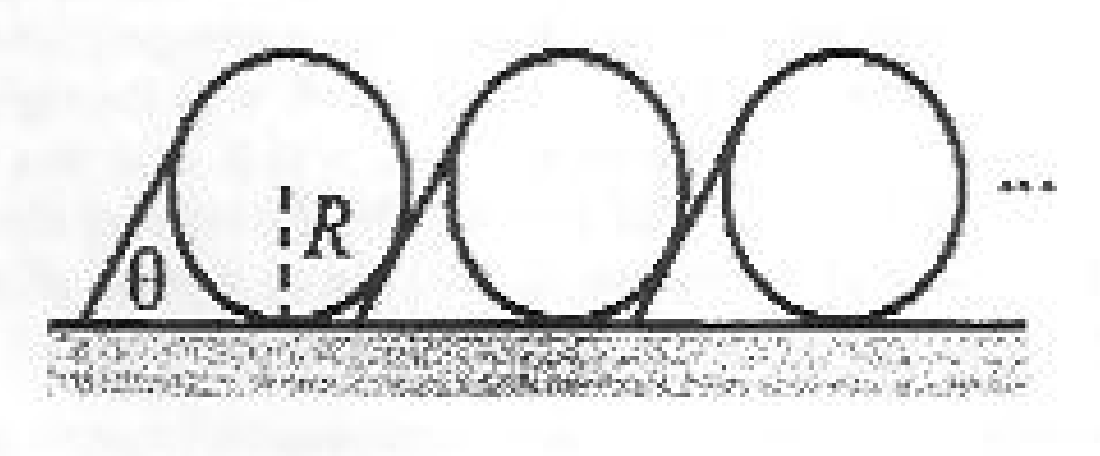
\includegraphics[width=0.7\linewidth]{spho_book_TYS_images/2011q5.png}
	\caption{Stick on a circle}
\end{figure}
(2) A large nunber of sticks (with mass density per unit length $\rho$) and circles (with radius $R$) lean on each other, an shown in the Figure below. Each stick makes an angle $\theta$ with the horizontal and is tangent to a circle at its upper end. The sticks are hinged to the ground, and every other surface is frictionless unlike in the first part of this question in (i)]. In the limit of a very large number of sticks and circles, what is the normal force between a stick and the circle it rests on very far to the right? (Assume that the last circle leans against a wall, to keep it from moving) [6]


\subsection{Solution 5}
Q4(ii) Referering to the sane dergram, ne are aive allomed fo vary $x_{0}, x, y$ such that they satisty 4 anneradht guotars,

From (2),
$$
\begin{array}{l}
	x-x_{1}=\frac{y_{1}}{m_{00}} \\
	x=\left(\frac{y}{m x_{0}}+1\right) x_{1} \\
	\quad=\left(\frac{f_{2}\left(\frac{m x_{0}}{f_{1}}-M+1\right)}{m_{x_{0}}}+1\right) x_{1}
\end{array}
$$$$
n-+h \text { ball }
$$ ball and surdes or lall and Aloor,
$$
N_{n}=N_{n}^{\prime}
$$
Ther conside fle $(n+1)$ th stick.
consille torque abent the hinge,
$$
\begin{array}{l}
	N_{n+1} l=\frac{m g l}{2} \cos \theta-N_{n} R \tan \frac{\theta}{2}=0 \\
	\text { Whth } l=\frac{R}{\tan \frac{\theta}{2} .} \\
	\frac{N_{n+1} R}{\tan \frac{\theta}{2}}-\frac{m g R}{2 \tan \theta} \cos \theta-N_{n} R \tan \frac{\theta}{2}=0 . \\
	N_{n+1}=N_{n} \tan ^{2} \frac{\theta}{2}+\frac{m g}{2} \cos \theta
\end{array}
\begin{aligned}
	N_{n} &=N_{n-1} \tan ^{2} \frac{\theta}{2}+\frac{m g}{2} \operatorname{as} \theta \\
	&=\left(N_{n-2} \tan ^{2} \frac{\theta}{2}+\frac{m}{2} \cos \theta\right) \tan ^{2} \theta_{2}+\frac{m g}{2} \cos \theta \\
	&=N_{n-2}\left(\tan ^{2} \frac{\theta}{2}\right)^{2}+\frac{m g}{2} \operatorname{as} \theta\left(1+\tan ^{2} \frac{\theta}{2}\right) \\
	&\left.=N_{n-3}\left(\tan ^{2} \frac{\theta}{2}\right)^{3}+\frac{m g \cos \theta\left(1+\tan ^{2} \theta+\tan \frac{4 \theta}{2}\right)}{2}\right) \\
	&=N_{n-4}\left(\tan ^{2} \frac{\theta}{2}\right)^{4}+\frac{m g}{2} \cos \theta\left(1+\tan ^{2} \frac{\theta}{2}+\tan ^{4} \frac{\theta}{2}+\tan ^{6} \frac{\theta}{2}\right) \\
	&=\cdots \\
	&=N_{0}\left(\tan ^{2} \frac{\theta}{2}\right)^{n}+\frac{m g}{2} \operatorname{as} \theta\left(\frac{1-\tan ^{2 n} \frac{\theta}{2}}{1-\tan ^{2} \frac{\theta}{2}}\right)
\end{aligned}
$$
A, $n \rightarrow \infty, \quad\left(\tan ^{2} \frac{\theta}{2}\right)^{n} \rightarrow 0 \quad$ because $\theta<\pi / 2$
$\lim _{n \rightarrow \infty} N_{n}=\frac{m g}{2} \frac{\operatorname{asc} \theta}{1-\tan ^{2} \frac{\theta}{2}}$
$=\frac{\rho R g}{2} \frac{\cos \theta}{\left(1-\tan ^{2} \frac{\theta}{2}\right) \tan \frac{\theta}{2}}$
$=\frac{\sin g}{2} \frac{\cos \theta \cos ^{2} \frac{\theta}{2}}{\left(\cos ^{2} \frac{\theta}{2}-\sin ^{2} \frac{\theta}{2}\right) \tan \frac{\theta}{2}}$
$=\frac{\rho^{2 g}}{2} \cos ^{2} \frac{\theta}{2} \cot \frac{\theta}{2}$




\subsection{Question 6}
6. An aluminum rod $0.500 \mathrm{~m}$ in length and with a cross-sectional area of $2.50 \mathrm{~cm}^{2}$ is inserted into a thermally insulated vessel containing laguid helinm at $4.20 \mathrm{~K}$. The rod is initidy at $300 \mathrm{~K}$. \\
(i) If half of the rod is inserted into the helium, how many liters of helium boil off by the time the inserted half cools to $4.20 \mathrm{~K} ?$ (Assume the upper half does not yet cool.) [4] \\
(ii) If the upper end of the rod is maintained at $300 \mathrm{~K}$, what is the approximate boil-off rate of liquid helium after the lower half has reached $4.2 \mathrm{~K} ?$ (Aluminum has thermal conductivity of $31.0 \mathrm{~J} \mathrm{~s}^{-1} \mathrm{~cm}^{-1} \mathrm{~K}^{-1}$ at $4.2 \mathrm{~K}$ You may ignore its temperature variation. Note that aluminum has a specific heat capacity of $902 \mathrm{~J~kg}^{-1} \mathrm{~K}^{-1}$ and density of $2700 \mathrm{~kg} \mathrm{~m}^{-3}$. The density of liquid helium is $125 \mathrm{~kg} \mathrm{~m}^{-3}$.) [4] \\


\subsection{Solution 6}


\subsection{Question 7}

7. A soap film $(n=1.33)$ is contained within a rectangular wire frame. The frame is held vertically so that the film drains downward and forms a wedge with flat faces. The thickness of the film at the top is essentially zero. The film is viewed in reflected white light with near-normal incidence, and the first violet (the wavelength is 420 nm) interference band is obsarved $3.00$ cm from the top edge of the film. \\
(j) Locate the first red $(\lambda=600 \mathrm{~nm})$ interference band. [4] \\
(ii) Determine the film thickness at the positions of the violet and red bands. [3] \\
(ii) What is the wedge angle of the film? [3] \\

\subsection{Solution 7}

\subsection{Question 8}

8. A solenoid of length $2 \ell$ has an inner radius $R_{1}$ and arrouter radius $R_{2}$. The current through the solenoid is $I$. \\
(i) Show that the magnetic flox density, $E$ at the center of the solenoid is
$$
B=\kappa n I \ell \frac{\alpha+\left(\alpha^{2}+\beta^{2}\right)^{1 / 2}}{1+\left(1+\beta^{2}\right)^{1 / 2}}
$$
where $n$ is the number of turns per square meter and $\alpha$ and $\beta$ are functions of $R_{1}, R_{2}$ and $L$. Write down the exprestion for $\alpha$ and $\beta$. State the value of $\kappa$. \\
(ii) Show that the length of the wire is
$$
\ell=n V=2 \pi n\left(\alpha^{m_{1}}-1\right) \beta^{m_{1}} R_{1}^{m_{2}}
$$
where $V$ is the volume of the winding and $m_{1}, m_{2}$ and $m_{3}$ are exponents thet need to be determined. State the value of $m_{1}, m_{2}$ and $m_{3}$. \\
(iii) Show that the $B$ field at the center of the solenoid can be written as
$$
B=G\left(\frac{P \lambda \sigma}{R_{1}}\right)^{1 / 2}
$$
where $G$ depends on the geometry, $P$ is the dissipated power, $\lambda=\pi \pi r^{2}$ is the filling factor or fraction of the coil cross sechon oocupied by the conductor, $r$ is the radius of the wire and $\sigma$ is the conductivity. [4]

\subsection{Solution 8}

\subsection{Question 9}
9. (a) A large block, with a second block sitting on top, is connected to a spring and executes horizontal simple harmonic motion as it slides across a frictionless surface with an angular frequency $\omega$. The coefficient of static friction between the two blocks is $\mu_{s}$. Derive a formula for the maximum amplitude of oscillation that the system can have if the upper block is not to slip. (Assume that the mass of the spring is negligible.) [6] \\
(b) A pencil of length $L_{1}$ with the pencil point at one end and an eraser at the other end, is initially standing vertically on a table with the pencil point on the table. The pencil is let go and falls over. Derive a formula for the speed with which the craser strikes the table, assuming that the pencil point does not move. [4]

\subsection{Solution 9}

\subsection{Question 10}
10. (a) The Oscillation Project with Emulsion-tRacking Apparatus (OPERA), an experiment designed to test neutrino ostillations and exploiting the high energy muon neutrino produced at CERN Super Proton Synchrotron in Geneva and pointing towards Gran Sasso in Italy, reported that the time of flight messurements indicated that muon neutrinos trave! at speed $v$ which is faster than the speed of light with $\beta=\frac{v}{c}=1+1.48 \times 10^{-5}$, where $c$ is the speed of light in vacua. Show that it is possible for an observer moving relative to the Earth starting at CERN and moving towards Gran Sasso at some critical speed $u$ to see the muon neatrino moving backwards from Gran Sasso towards CERN and determine this critical speed.\\
(b) A moving rod is observed to have a length of $2.00 \mathrm{~m}$ and to be oriented at an angle of $30.0^\circ$ with respect to the direction of motion, as shown in the Figure below. The rod has a speed of $0.995~c$.
\begin{figure}
	\centering
	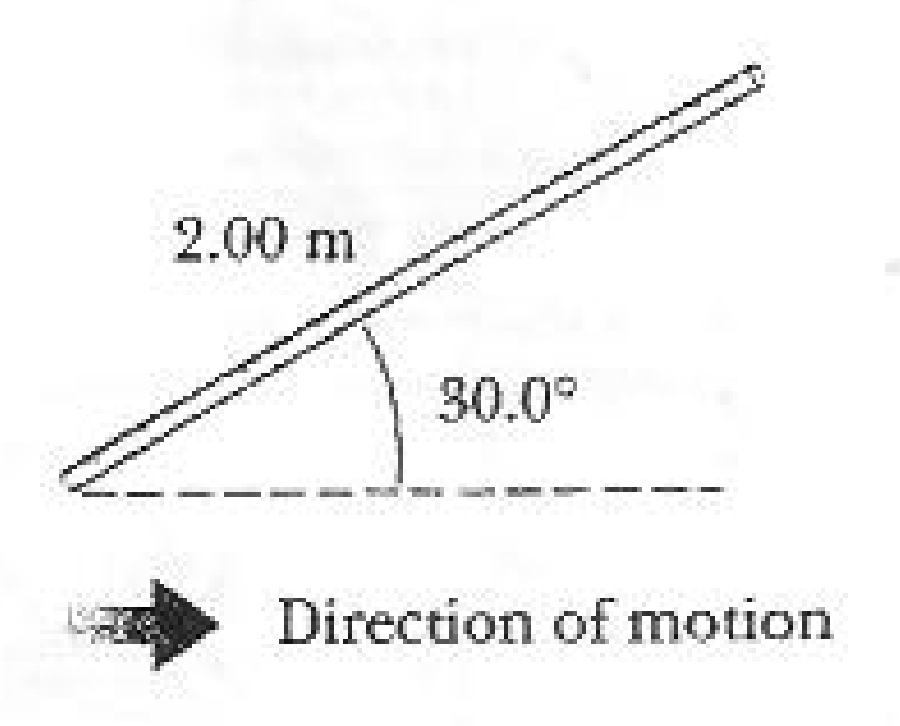
\includegraphics[width=0.7\linewidth]{spho_book_TYS_images/2011q10.png}
	\caption{Relativistic Rod}
\end{figure}
(i) Determine the proper length of the rod. [3] \\
(ii) What is the orientation angle in the proper frame? [3] \\

\section{2012}

\subsection{Question 1}
1. A platform scale is calbrated to indicate the mass in $\mathrm{kg}$ of an object placed on it. Particles fall from a height of $3.5 \mathrm{~m}$ and collide with the balance pan of the scale. Assuming that the collisions are elastic and that the particles rebound upwards with the same speed they had before hitting the pan, determine the average scale reading if each particle has mass $110 \mathrm{~g}$ and collisions occur at the rate of $42 \mathrm{~s}^{-1}$. [8] \\

\subsection{Question 2}
2. A collection of $N$ identical blocks, each of mass $M$, are connected by unstretchable ropes of negligible mass. The blocks are on a horizontal surface. An external force $F_{0}$ acts on Block 1, pulling it horizontally to the right with constant velocity. What is the tension in the rope connecting Block $n$ to Block $n+1$, if
\begin{figure}
	\centering
	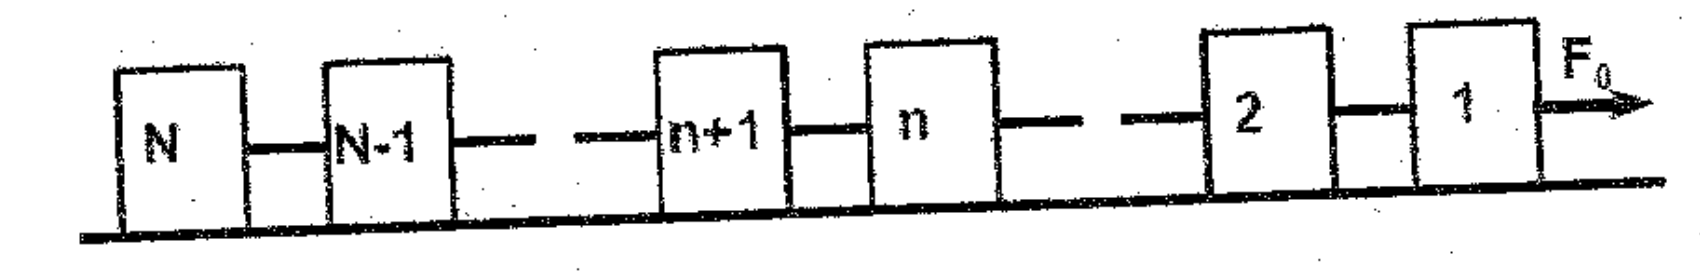
\includegraphics[width=0.7\linewidth]{spho_book_TYS_images/2012q1.png}
	\caption{$N$ identical blocks}
\end{figure}
(i) There is no friction between the blocks and the surface? [3] \\
(ii) The coefficient of kinetic friction between each block and the surface is $\mu_{k}$? ( $F_{0}$ large enough to accelerate the blocks despite the friction.) [5] \\

\subsection{Question 3}
3. A pendulum bob is constructed by taking a thin, uniform-density circular ring of mass $M$ and radius $R$ and affixing a straight, thin, uniform density rod of mass ${m}$ and length $2 R$ across its diameter as shown in the diagram. The pendulum hangs in a vertical plane from a frictionless pivot that can be attached to the ring at any point. The pivot allows the bob to swing either in the plane of the bob or in the plane perpendicular to the bob. Assume the angular amplitude is small.

(i) What swinging configurations givd the maximum period? [4]
(ii) What swinging configurations give the minimum period? [4]
(iii) Find the ratio of the maximum period to the minimum period. [2]

\subsection{Question 4}
4. The distance from the centre of the Earth to the poles is $21 \mathrm{~km}$ shorter than the radius of the equator. A one second pendulum is taken from the equator (at sea level) to the North Pole. Make a rough estimate of its change in period. You may assume for the purposes of your calculation that the Earth has a constant density. [6]

\subsection{Question 5}
5. A square lattice of identical resistances (1 ohm along each edge) is wrapped around an infinite cylinder in such a way that $N$ resistances are placed along the cross sectional circle of the cylinder. What are the resultant resistances between two adjacent lattice points in the "axial" and in the "circumferential" directions? [12] \\
First consider the cases $N=2, N=3$, and the limit $N \rightarrow \infty$

\subsection{Question 6}
6. An infinitely long perfectly conducting straight wire of radius $r$ carries a constant current $i$ and charge density zero as seen by a fixed observer $A$. The current due to an electron stream of uniform density moving with high (relativistic) velocity $U$. A second observer travels parallel to the wire with high (relativistic) velocity $v . \mathrm{As}$ seen by the second observer, $B$, \\
(a) What is the electrornagnetic field? [3] \\
(b) What is the charge density in the wire implied by this field? [3] \\
(c) With what velocities do the electron and ion streams move? [4] \\
(d) How do you account for the presence of a charge density seen by $B$ but not by $A$? [4]

\subsection{Question 7}
7. When a perfect monatomic gas expands adiabatically (no heat interchange with its surroundings) the pressure and volume of the gas are related by the formula:
$$
P_{1} V_{1}^{\gamma}=P_{2} V_{2}^{\gamma}
$$
where $\gamma$ in this case is $5 / 3$ and $P_{1}, V_{1}, P_{2}, V_{2}$ refer to the initial and final states of the volume and pressure of the gas . A helium balloon at atmospheric pressure is allowed to rise rapidly to a height such that the external pressure is half atmospheric pressure. The envelope of the balloon is at all times loose, of negligible mass, and regarded as a perfect heat insulator. \\
(i) Calculate the ratio of the initial to final volume of the balloon. \\
(ii) If the initial temperature of the gas was $300 \mathrm{~K}$, what will be its new temperature? [5] 

\subsection{Question 8}
8. It is well known in classical (nonrelativistic) electrodynamics that an electron traces out a circular orbit in a uniform magnetic field. But what if it is not all alone? Examine two electrons in a homogeneous magnetic feld moving in the plane perpendicular to the field lines. Under suitably chosen initial conditions the two electrons are found to move along the same circular orbit. Determine the radius of this circle. Are there further periodic solutions? What happens in the case of an electron and a positron? Can the two annihilate (i.e. encounter), and if so, under what initial conditions? [12]

\subsection{Question 9}
9. A cylindrical piece of steel, of diameter $0.4 \mathrm{~mm}$, is lowered very carefully on to water. Show that it may float horizontally with approximately half its volume above the free surface of the liquid. Assume that the angle of contact is $\pi$ radian. (Take the density of steel to be $8.5 \times 10^{3} \mathrm{~kg} \mathrm{~m}^{-3}$ and the surface tension of water to be $7.0 \times 10^{-2} \mathrm{~N} \mathrm{~m}^{-1}$. [8]

\subsection{Question 10}
10. In a Young's double slit experiment, the region between screen and slits is immersed in a liquid whose refractive index varies with time $t$ (in seconds) as $n_{\ell}=2.50 - 0.25 t$ until it reaches a steady state value $1.25$. The distance between the slits and the screen is $D=1.00 \mathrm{~m}$ and the distance between the slits $S_{1}$ and $S_{2}$ is $d=2.00 \times 10^{-3}$ m. A glass plate of thickness $t_{g}=3.60 \times 10^{-5} \mathrm{~m}$ and refractive index $n_{g}=1.50$ is introduced in front of one of the slits. Note that the illuminations at $S_{1}$ and $S_{2}$ are from coherent sources with zero phase difference.

\begin{figure}
	\centering
	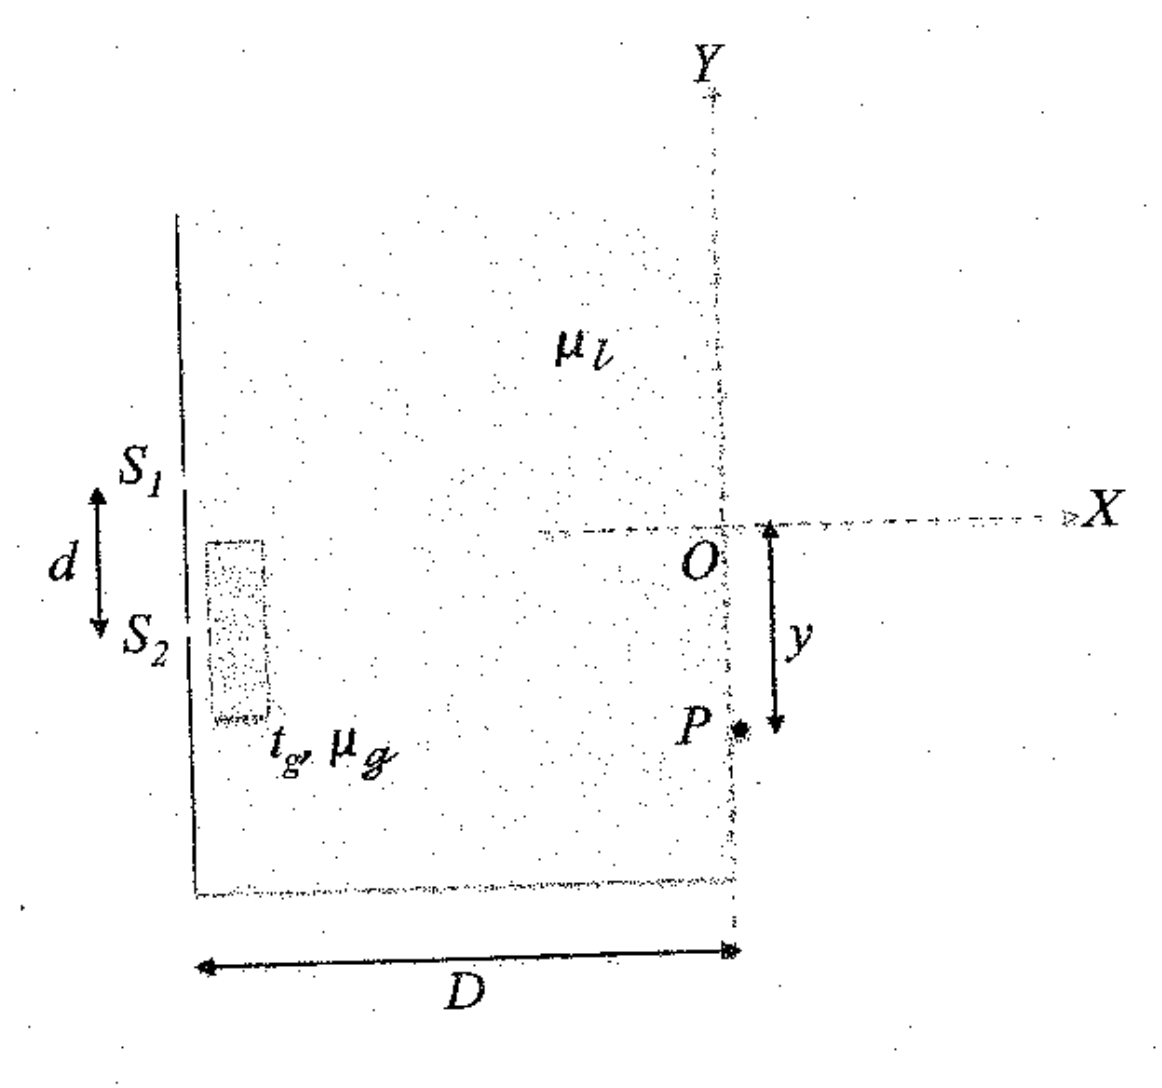
\includegraphics[width=0.5\linewidth]{spho_book_TYS_images/2012q10.png}
	\caption{Modified Young's Double Slit}
\end{figure}

(i) Consider the point $P$ on the screen at a distance $y$ from O $(S_{1} O=S_{2} O ; O P=y)$. Obtain the expression for the optical path difference $\Delta x$ in terms of the refractive indices. [3] \\
(ii) If $P$ is the central maximum. Obtain the expression for $y$ as a function of time $t$. [3] \\
(iii) Obtain the time $t_{m}$ when the central maximum is at a point $O$, equidistant from $S_{1}$ and $S_{2}$, i.e. $S_{1} O=S_{2} O$ [3] \\
(iv) Determine the speed, $v$ of the central maximum when it is at $O$. [3]

\section{2013}

\subsection{Question 1}
1. The first explosion of the atomic bomb was conducted near Alamogoro, New Mexico on July 16, 1945. The Figure below shows a picture of the approximately spherical shockwave $25 \mathrm{~msec}$ with the tick marks indicating $100 \mathrm{~m}$ Using dimensional analysis, find an

\begin{figure}
	\centering
	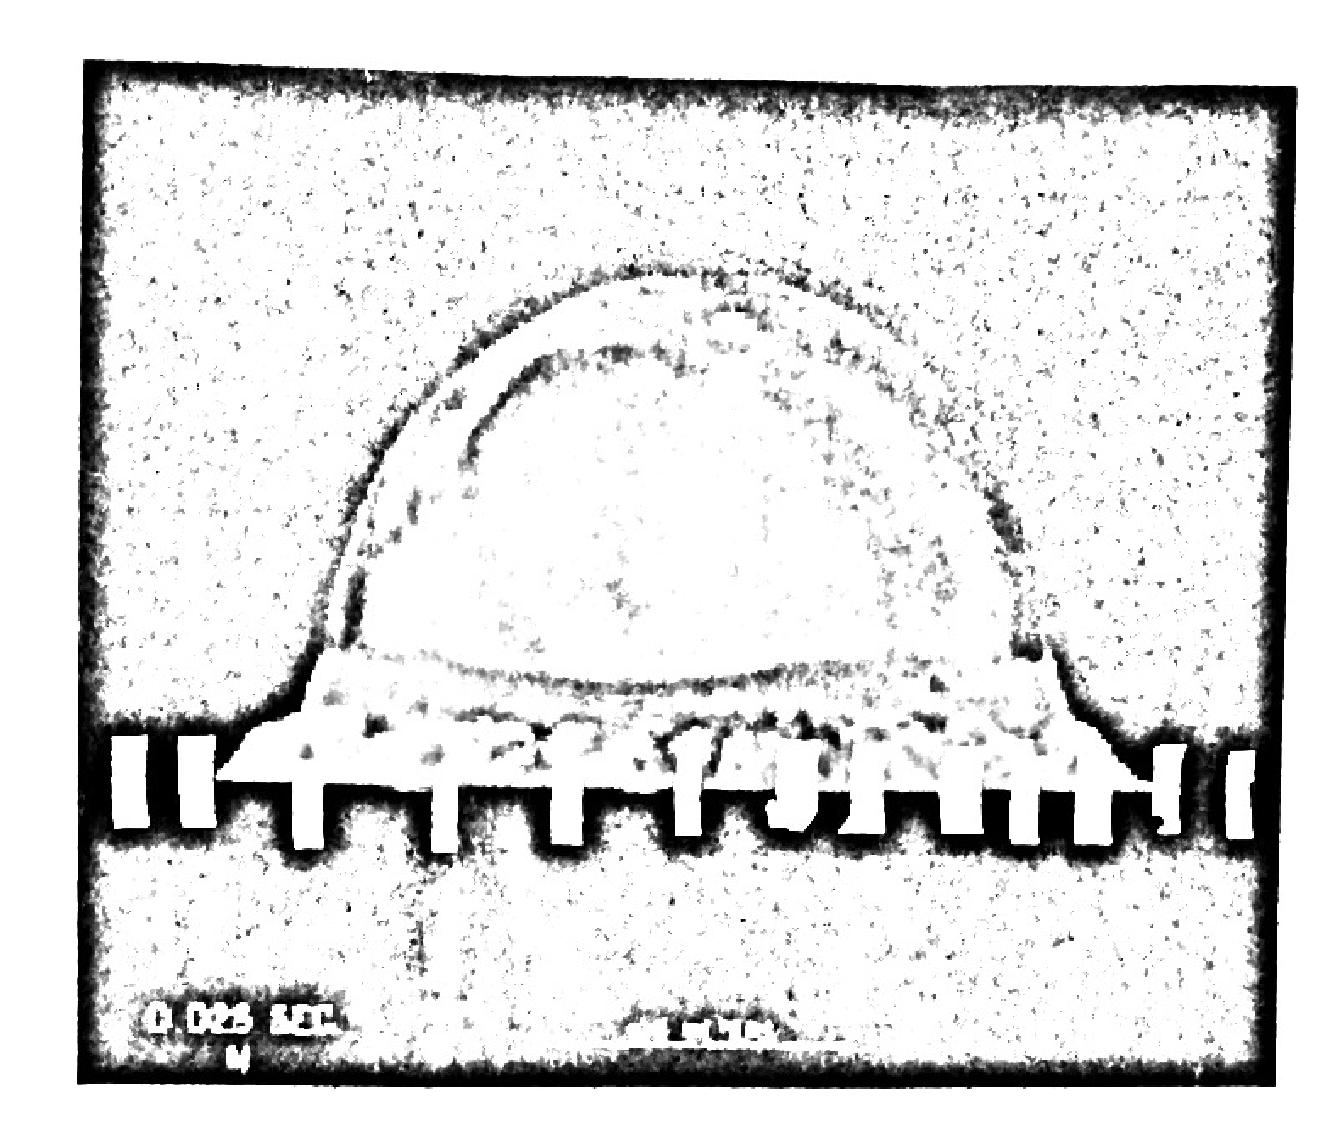
\includegraphics[width=0.5\linewidth]{spho_book_TYS_images/2013q1.png}
	\caption{Camera shot of the bomb after 25 msec.}
\end{figure}

expression for the radius of the shockwave, $R$, as a function of the density $\rho$ of the medium (i.e. the air) through which the shock wave travels, the energy of the explosion, $E$ and the time, $\mathrm{t}$, that elapsed since the explosion.
Assuming that the proportionality constant is unity (i.e. 1), as predicted by Sir Geoffrey Taylor, and assuming that the density of air, $\rho$, is $1.2 \mathrm{~kg} \mathrm{~m}^{-3}$, and that the explosion of $1000 \mathrm{~kg}$ of TNT releases an energy of $4.184 \times 10^{9} \mathrm{~J}$, estimate, from the picture, the approximate energy of this explosion expressed as tons $(1000 \mathrm{~kg})$ of TNT equivalent. [8]

\subsection{Question 2}

2. During a discussion in a physics meeting, Einstein used this problem to illustrate the notion of adiabatic invariant. A pendulum, made up of a ball of mass $M$ suspended from a pivot by a light string of length $L$, is swinging freely in a vertical plane. By what factor does the amplitude of the oscillations change if the string is shortened very slowly by a factor of $2 ?$
$[10]$

\subsection{Question 3}
3. A rocket is projected straight up and explodes into three equally massive fragments just as it reaches the top of its flight. One of the fragments is observed to come straight down to the ground in time $t_{1}$ while the other two land at time $t_{2}$ after the burst. Find the height $h\left(t_{1}, t_{2}\right)$ at which the fragmentation occurred. [10]

\subsection{Question 4}
4. An early but unfortunately incorrect model of the hydrogen atom suggested by J.J. Thomson postulated that the hydrogen atom is a positive cloud of charge $+e$ uniformly distributed throughout a volume of a sphere of radius $R$ with the clectron represented by a equal magnitude but negative point charge $-e$ at the center of the sphere.  \\
(i) Show that the electron is in equilibrium at the center and that if displaced a small distance $r<R$ would experience a restoring force of the form $F=-K r$ where $K$ is a constant. Determine $K$. [3] \\
(ii) Find an expression for the frequency of the simple harmonic oscillations that the electron of mass $m_{e}$ would undergo if displaced a small distance from the center and released. [3] \\
(iii) Calculate a numerical value for $R$ that would result in a frequency of $2.47 \times 10^{15}$ $\mathrm{Hz}$, the frequency of light radiated in the most intense line of the hydrogen spectrum. [3]

\subsection{Question 5}
5. A "perfect" rocket engine combines matter and antimatter in a controlled way to yield photons (high energy gamma rays) all of which are directed out of a spaceship. Suppose we start with a spaceship of initial mass $M_{0}$ at rest, and that at burnout, the remaining spaceship moves at speed $v$ and has mass $m$ equal to the fraction $f$ of the original mass. You may take the speed of light $c=1$ and $\gamma=1 / \sqrt{1-v^{2}}$. \\
(i) What is the total energy of this system initially? Let $E_{\text {rad }}$ stand for the total energy of radiation after the burnout. Find an expression for the total energy of the system after the burnout and set up the conservation of energy equation. [2] \\
(ii) Write down the equation for the conservation of momentum. [2]\\
(iii) Show that $\gamma f+\gamma v f=1$. [2] \\
(iv) Show that $\gamma v=\sqrt{\gamma^{2}-1}$ so that $f^{2}-2 \gamma f+1=0$. [3]
(v) What is the value of $f$ if $\gamma=10 ?$ Is it possible to construct a spaceship whose shell and payload with this $f$? [3] \\
(vi) Using $f$ obtained above for $\gamma=10$, show that the total energy of the emitted radiation is less than the mass of fuel consumed. Explain why. [3]


\subsection{Question 6}
6. On a smooth and insulating large ring of radius $R$, there is a small ring of mass $m$ and carrying charge $q$. The large ring is placed horizontally and in a uniform magnetic field of strength $B_{0}$ and perpendicular to the ring plane. Starting at $t=0$, the magnetic field is changed to $B(t)=B_{0}+\alpha t$. Find the force of the small ring acting on the big ring afterwards and describe the motion of the small ring [10]

\subsection{Question 7}
7. Three polarizing disks whose planes are parallel are centered on a common axis. The direction of the transmission axis in each case is shown in Figure 2 relative to the common vertical direction. A plane-polarized beam of light with $E_{0}$ parallel to the vertical reference direction is incident from the left on the first disk with intensity $I_{0}=10.0$ in some arbitrary units. Calculate the transmitted intensity I when
(i) $\theta_{1}=20.0^{\circ}, \theta_{2}=40.0^{\circ}$, and $\theta_{3}=60.0^{\circ} ;$
(ii) $\theta_{1}=0^{\circ}, \theta_{2}=30.0^{\circ}$, and $\theta_{3}=60.0^{\circ} ;$
(iii) If $\theta_{1}=0^{\circ}$ and $\theta_{3}=60.0^{\circ}$, find the angle $\theta_{2}$ so that maximum intensity passes through the three polarizers.

\begin{figure}
	\centering
	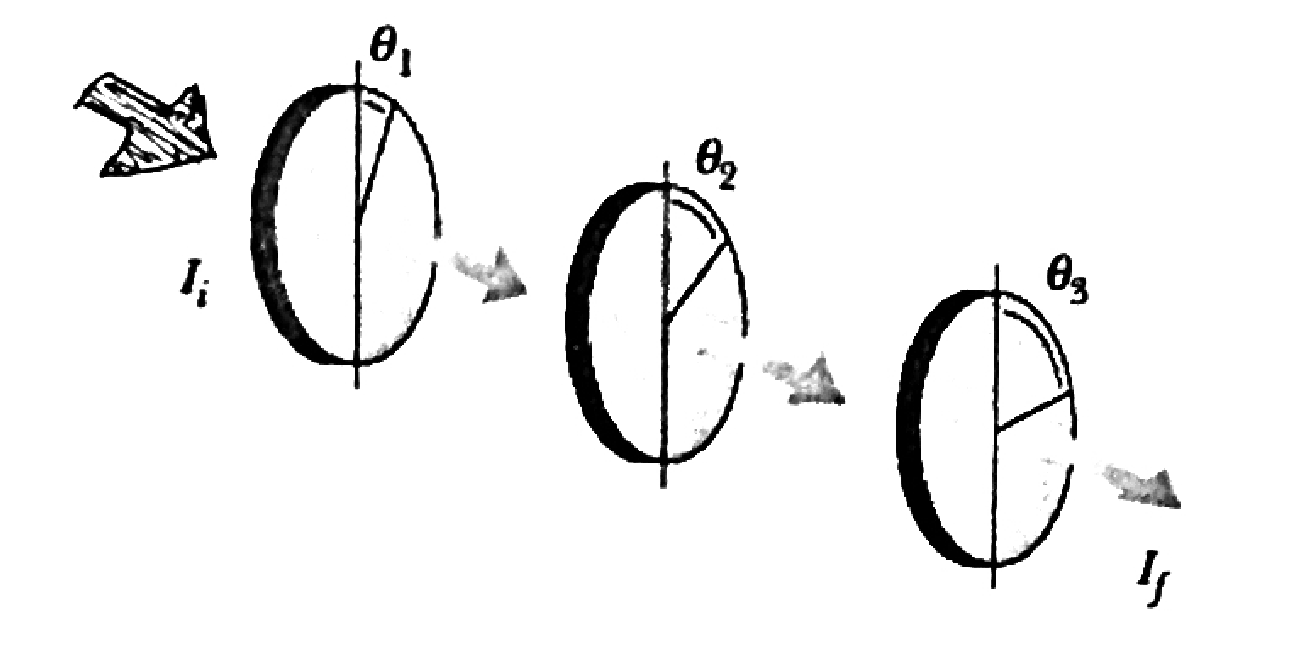
\includegraphics[width=0.5\linewidth]{spho_book_TYS_images/2013q7.png}
	\caption{Three polarizing disks whose planes are parallel are centered on a common axis.}
\end{figure}


\subsection{Question 8}
8. Two parallel rails with negligible resistance are $10.0 \mathrm{~cm}$ apart and are connected by a $5.00 \Omega$ resistor. The circuit also contains two metal rods having resistances of $10.0$ $\Omega$ and $15.0 \Omega$ sliding along the rails (see figure 3). The rods are pulled away from the resistor at constant speeds of $4.00 \mathrm{~ms}^{-1}$ and $2.00 \mathrm{~ms}^{-1}$, respectively. A uniform magnetic field of magnitude $0.0100 \mathrm{~T}$ is applied perpendicular to the plane of the rails. Determine the current in the $5.00 \Omega$ resistor. [8]


\subsection{Question 9}
9. In the figure below, the switch is closed for $t<0$, and steady-state conditions are established. The switch is opened at $t=0$.\\
(i) Find the initial voltage $\mathcal{E}_{t}$ across $L$ just after $t=0$. Which end of the coil is $\mathrm{nt}$ the higher potential: a or b? [3]\\
(ii) Sketch graphs of the currents in $R_{1}$ and in $R_{2}$ as a function of time, treating the steady-state directions as positive. Show the values before and after $t=0$. [5] \\
(iii) How long after $t=0$ would the current across $R_2$ be $2.00 \mathrm{~mA}$? [2]


\begin{figure}
	\centering
	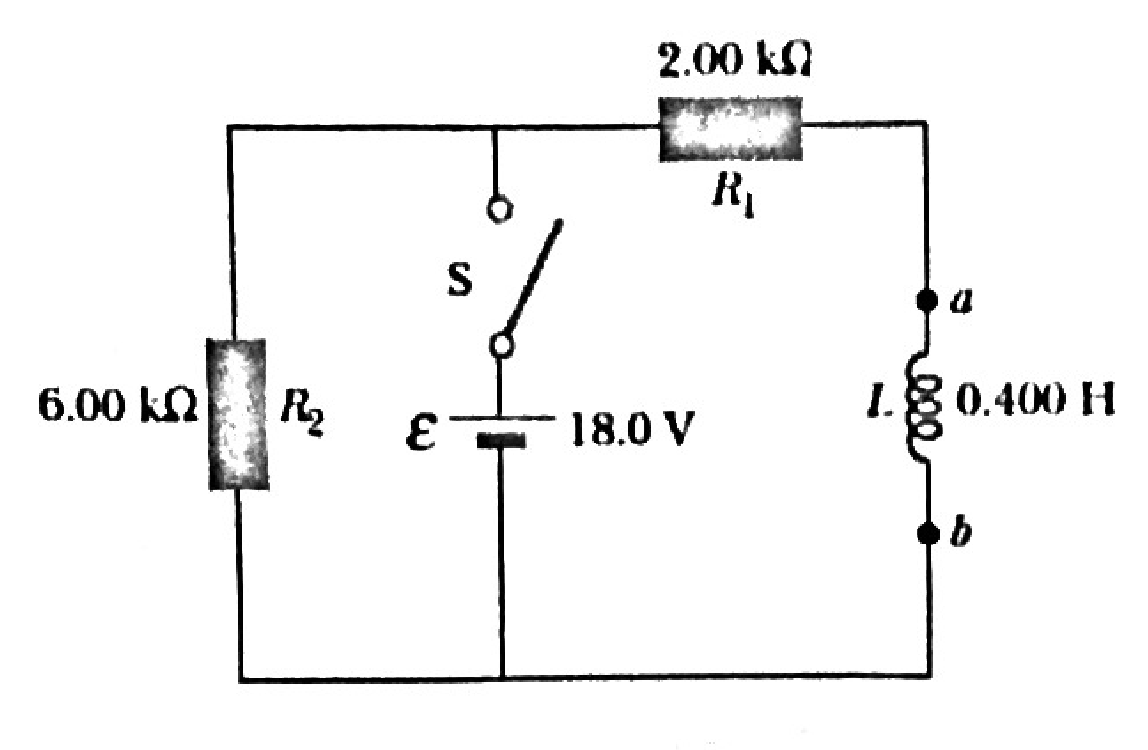
\includegraphics[width=0.5\linewidth]{spho_book_TYS_images/2013q9.png}
	\caption{Circuit}
\end{figure}

\subsection{Question 10}
10. A transparent cylinder of radius $R=2.00$ m has a mirrored surface on its right half, as shown in Figure 5. A light ray traveling in air is incident on the left side of the cylinder. The incident light ray and exiting light ray are parallel and $d=2.00 \mathrm{~m}$. Determine the index of refraction of the material. [10]

\begin{figure}
	\centering
	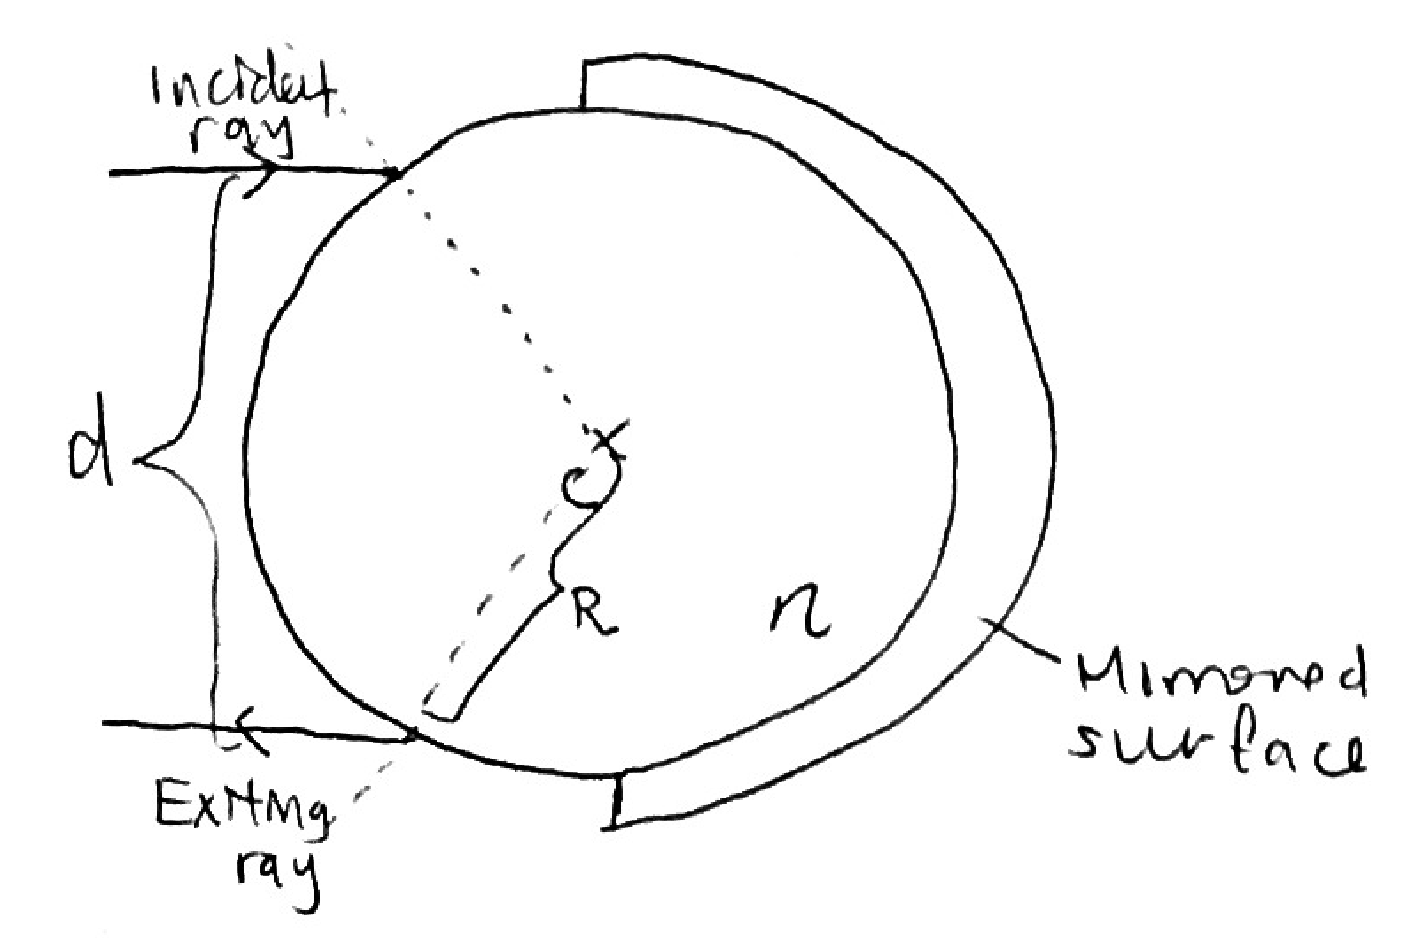
\includegraphics[width=0.5\linewidth]{spho_book_TYS_images/2013q10.png}
	\caption{Transparent cylinder with mirrored surface}
\end{figure}

\section{2014}
\subsection{Question 1}
1. Yo-Yo! \\ A yo-yo of mass $M$ lies on a smooth horizontal table as shown below. The moment of inertia about the center may be taken as $\frac{1}{2} M A^{2} .$ A string is pulled with force $F$ from the inner radius $B$ as indicated below.

\begin{figure}
	\centering
	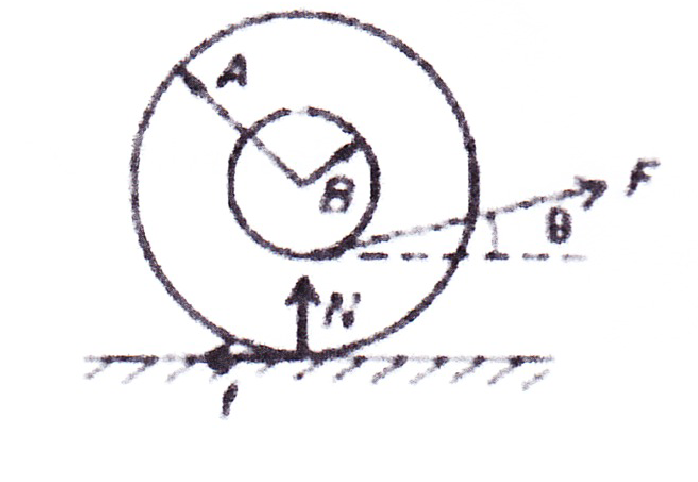
\includegraphics[width=0.5\linewidth]{spho_book_TYS_images/2014q1.png}
	\caption{Yo-yo on a smooth table}
\end{figure}

(a) Draw diagrams to show which direction the yo-yo will roll if $\theta=0, \pi / 2, \pi .$ [2] \\
(b) For what value of $\theta$ will the yo-yo slide without rolling independent of the roughness (coefficient of friction) of the table or the magnitude of $F$? [3] \\
(c) At what angle $\theta$ will the yo-yo roll, independent of the smoothness of the table? [5]

\subsection{Question 2}
2. Yo-yo continued \\ A yo-yo is pulled by its string along a horizontal surface without slipping. The horizontal velocity of the end of the string remains equal to $v .$ A bar is pivoted as shown and remains supported by the yo-yo. Find the angular speed of the bar $\omega$ as a function of the angle $\theta$. The outer and the inner radii of the yo-yo are $R$ and $r$ respectively. [10]

\begin{figure}
	\centering
	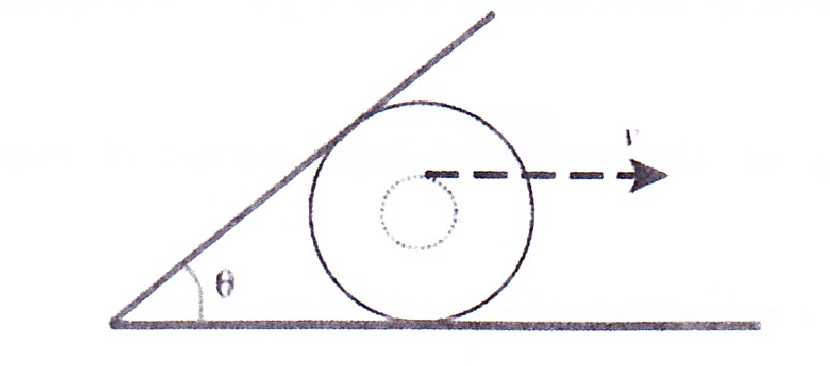
\includegraphics[width=0.5\linewidth]{spho_book_TYS_images/2014q2.png}
	\caption{Pulled yo-yo and supported bar}
\end{figure}

\subsection{Question 3}
3. Cylindrical capacitors \\
(a) A long cylindrical conductor has a radius $a$ and a linear charge density $+\lambda$. It is surrounded by a coaxial cylindrical conducting shell with inner radius $b$ and linear charge density $-\lambda .$ Calculate the capacitance per unit length for this capacitor, assuming that there is vacuum in the space between the cylinders. [4] \\
(b) Consider a cylindrical capacitor of length $l$ and of radii $a$ and $b$ as defined in (a), write down the conditions for which increasing $l$ by $10 \%$ would be more effective in increasing its capacitance than increasing $a$ by $10 \%$. [6] 

\subsection{Question 4}
4. Spring with mass \\ Problems involving springs often consider the springs to be massless. Of course, that is not true in reality. Here, we consider a spring with mass $M$, equilibrium length $L_{\circ}$, and spring constant $k$. \\
(a) The spring above has one end fixed and the other end moving with speed $v$. Assume the speed of points along the length of the spring varies linearly with distance $l$ from the fixed end. Assume also that the mass $M$ of the spring is distributed uniformly along the spring. Express the kinetic energy of the spring in terms of $M$ and $v$. [5] \\
(b) Write down the conservation of energy equation of a spring-mass system where the mass $m$ is moving at the end of a massless spring. What is the angular frequency $\omega$ for such a system? [2] \\
(c) By considering the procedure in (b), what is the angular frequency $\omega$ of the spring mentioned in (a)? If the effective mass $M^{\prime}$ of the spring is defined as $\omega=\sqrt{\frac{k}{M^{\prime}}}$ what is $M^{\prime}$ in terms of $M ?$ [3]

\subsection{Question 5}
5. Catching the wave \\
The speed of of a travelling wave $v$ along a string is a function of its tension $T$ and its linear mass density $\rho$ in the form $v=T^{\alpha} \rho^{\beta}$. \\
(a) Find $\alpha$ and $\beta$. [2] \\
(b) A uniform, almost inextensible string of length $l$ and total mass $M$ is suspended vertically and tapped at the top end so that a transverse impulse runs down it. At the same moment, a body is released from rest and falls freely from the top of the string. How far from the bottom does the body pass the impulse? [8]

\subsection{Question 6}
6. Playing with Horizontal Plates \\ A capacitor system is made of 2 horizontal square plates of sides $l$ separated by a distance $d$. \\
(a) If the uniform electric force field between them is $E$, what are the charges on the respective plates? Express your answer in terms of $E, l$ and other fundamental constansts.  [3] \\
(b) What is the force which the plates exert on each other when the potential difference between then is $V$ ? [2] \\
(c) The upper plate is fixed and the lower plate is resting on a table top and is free to move. The potential difference $V$ is gradually increased till the lower plate suddenly jumps up. Calculate the value of $V$ at which this occurs, given that the lower plate is made of alumninum (density $2.71 \times 10^{3} \mathrm{~kg} \mathrm{~m}^{-3}$ ) of thickness $8.00 \mu \mathrm{m}$ and that the initial separation is $12.7 \mathrm{~mm}$. [2] \\
(d) What is the energy per unit volume stored in the capacitor just before the lower plate jumps up? [2] 

\subsection{Question 7}
7. (a) At low temperatures, the heat capacity of a substance is dependent on its temperature. A thermally insulated piece of the substance is heated under atmospheric pressure by an electric cuurent so that it receives electric energy at a constant power $P$. This leads to an increase of the absolute temperature $T$ of the substance with time $t$ as $T(t)=T_{\circ}\left[1+a\left(t-t_{\circ}\right)\right]^{\frac{1}{3}}$. Here, $a, t_{\circ}$ and $T_{\circ}$ are constants. Determine the heat capacity $C_{p}$ of the substance as a function of temperature. [5] \\
(b) The index of refraction of glass can be increased by diffusing in impurities. It is then possible to make a lens of constant thickness. Given a disk of radius $a$ and thickness $d$, express the index of refraction $n(r)$ as a function of $n_{\circ}$ (refractive index at the centre of the lens), $r$ (radius from the centre of the lens), $d$ and $F$. You may assume $d<<a$. [5]

\subsection{Question 8}
8. (a) After falling a time $t$ in the atmosphere, an outer shell of a meteorite of thickness $x$ will have been heated significantly. The thickness can be estimated by dimensional analysis as the following thermodynamic parameters: $x=t^{\alpha} \rho^{\beta} c^{\gamma} k^{\sigma}$. \\
$\rho$ is the meteorite's density. \\
$c$ is the metorite's specific heat capacity. \\
$k$ is the meteorite's thermal conductivity. \\
Determine by dimensional analysis the value of the four powers $\alpha, \beta, \gamma$ and $\sigma$. [5] \\
(b) A beam of $10^{6} K_{l}$ mesons per second with $\beta=\frac{v}{c}=\frac{1}{\sqrt{2}}$ is observed to interact with a lead brick such that the $K_{l}$ mesons are being converted to $K_{s}$ mesons with the internal state of the lead brick identical before and after the reaction. The direction of motion of the incoming $K_{l}$ and outgoing $K_{s}$ may also be considered to be identical. Using
$$
\begin{aligned}
	&m\left(K_{l}\right)=5 \times 10^{8} \mathrm{eV} / c^{2} \\
	&m\left(K_{l}\right)-m\left(K_{s}\right)=3.5 \times 10^{-6} \mathrm{eV} / c^{2}
\end{aligned}
$$
give the magnitude and direction of the avearge force exerted on the brick by this process. [5] 

\subsection{Question 9}
9. Among the first successes of the interpretation by Ampere of magnetic phenomena, we have the computation of the magnetic field $B$ generated by wires carrying an electric current, as compared to early assumptions originally made by Biot and Savart. \\
A particularly interesting case is that of a very long thin wire, carrying a constant current $i$, made out of two rectilinear sections and bent in the form of a "V", with angular half-span $\alpha$ (see figure). According to Ampere's computations, the magnitude $\mathrm{B}$ of the magnetic field in a given point $\mathrm{P}$ lying on the axis of the "V", outside of it and at a distance $d$ from its vertex, is proportional to $\tan \left(\frac{\alpha}{2}\right) .$ Ampere's work was later embodied in Maxwell's electromagnetic theory, and is universally accepted. 

\begin{figure}
	\centering
	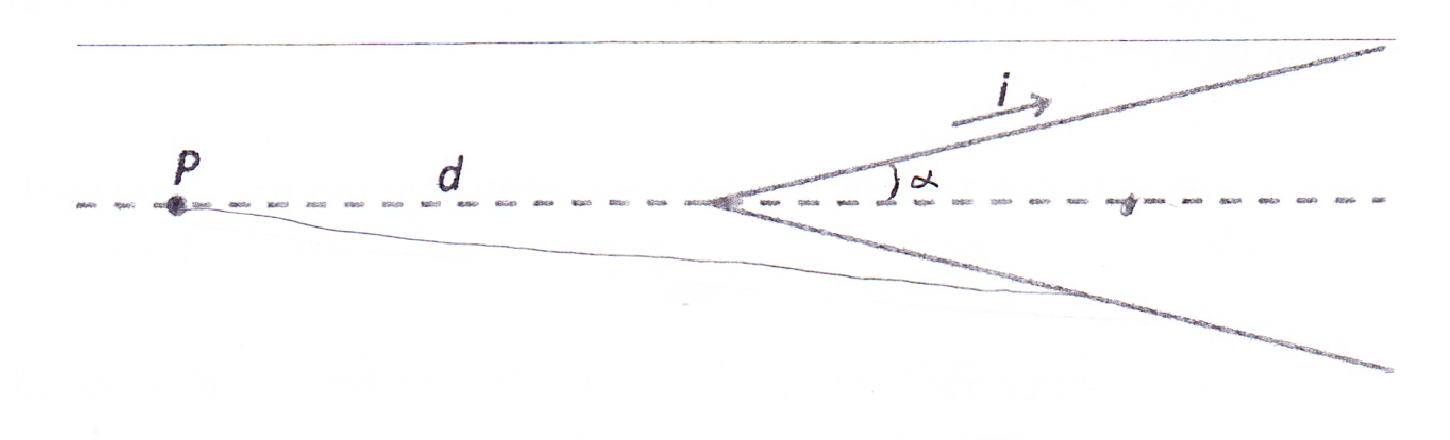
\includegraphics[width=0.5\linewidth]{spho_book_TYS_images/2014q9.png}
	\caption{Configuration of V-shaped wire}
\end{figure}

Using our knowledge of electromagnetism \\
(a) find an expression of the magnetic field $B$ in terms of the given quantities and any other relevant constants. Also, indicate the direction of the magnetic field [4] \\
(b) Compute the field at a point $\mathrm{P}^{*}$ symmetric to $\mathrm{P}$ with respect to the vertex i.e along the axis and at the same distance $d$ but inside the "V". [4] \\

\subsection{Question 10}
10. Radioactive dating of sample ${ }^{87} R b$ (element no 37) decays into the stable isotope ${ }^{87} S r$ (element no. 38) with a half life of $T_{\frac{1}{2}}=4.9 \times 10^{10}$ year, relative to the stable isotope ${ }^{86} \mathrm{Sr} .$ At the point of formation, the ratio ${ }^{87} \mathrm{Sr} /{ }^{86} \mathrm{Sr}$ was identical for all minerals in the sample while the ratio ${ }^{87} R b /{ }^{86} S r$ was quite different. As time passes on, the amount of ${ }^{87} R b$ decreases by decay, while consequently the amount of ${ }^{87} S r$ increases. As a result, the ratio of ${ }^{87} S r /{ }^{86} S r$ will be different today. In the following figure(a), the points on the horizontal line refer to the ratio ${ }^{87} R b /{ }^{86} S r$ in different minerals at the formation of the sample.

\begin{figure}
	\centering
	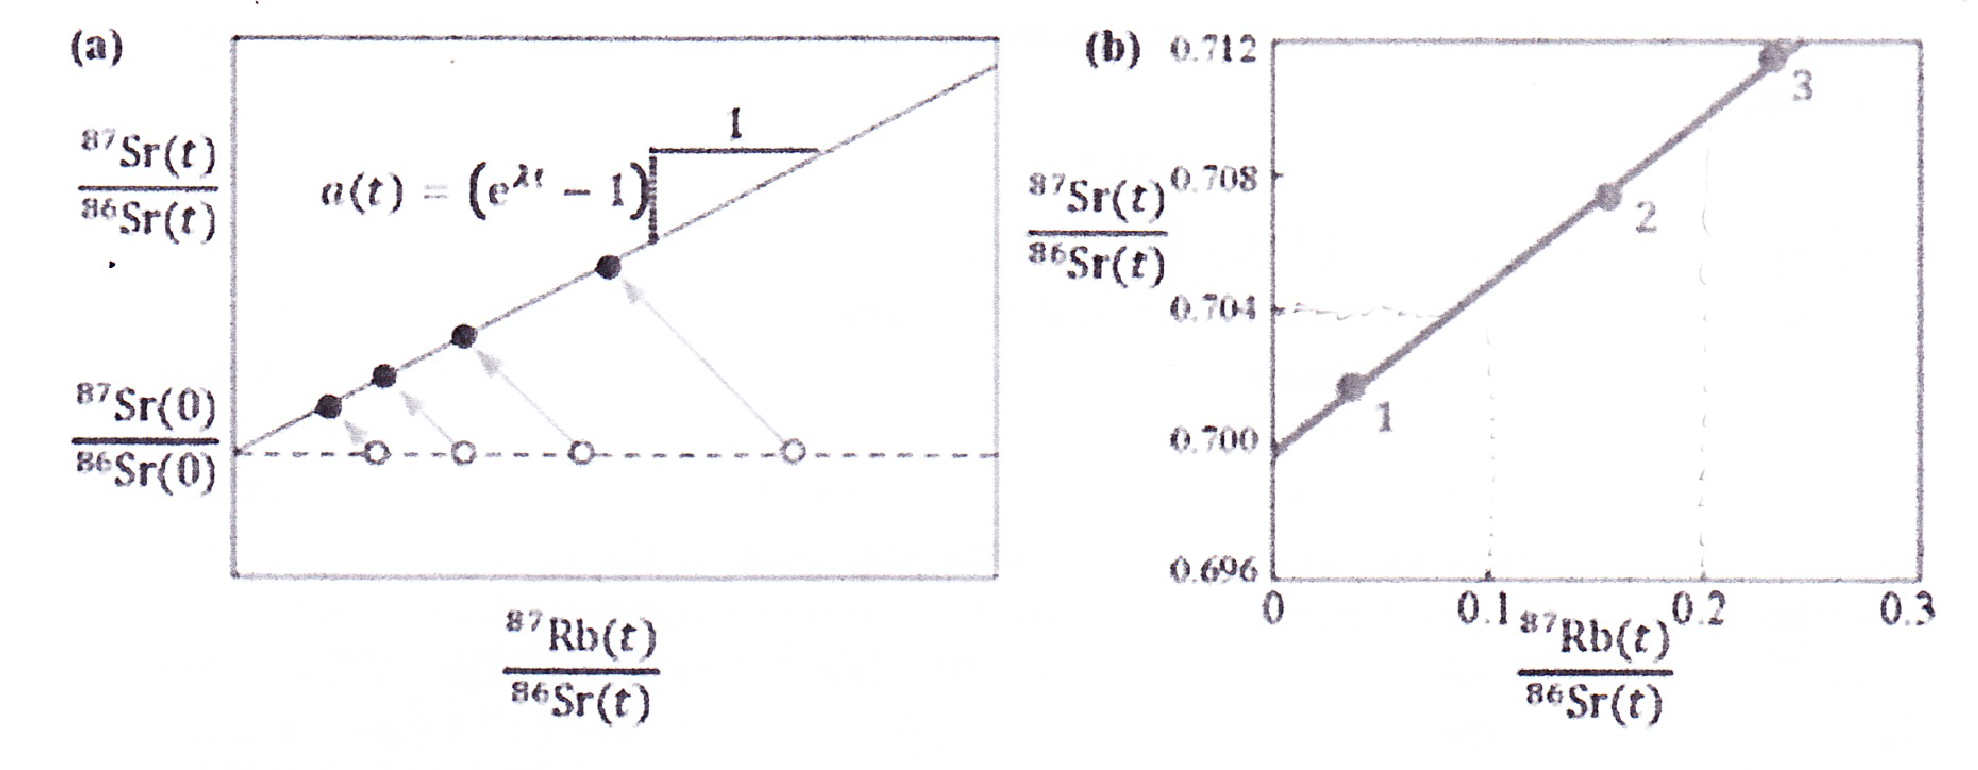
\includegraphics[width=0.5\linewidth]{spho_book_TYS_images/2014q10.png}
	\caption{(a) The ratio ${ }^{87} \mathrm{Sr} /{ }^{86} \mathrm{Sr}$ in different minerals at the time of formation, $t=0$ (open circles) and at present time (filled circles) (b) The isochron-line for three different minerals taken from the sample at present time}
\end{figure}
(a) Write down the nuclear reaction depicting the decay scheme for the transformation of ${ }_{37}^{87} R b$ to ${ }_{38}^{87} Sr$. \\
(b) Show that the present-time ratio ${ }^{87} \mathrm{Sr} /{ }^{86} \mathrm{Sr}$ was plotted versus the present-time ratio ${ }^{87} R b /{ }^{86} S r$ in different mineral samples from the same sample forms a straight line (the isochron line), with slope $a(t)=\left(e^{\lambda t}-1\right) .$ Here $t$ is the time since the formation of the minerals, while $\lambda$ is the decay constant inversely proportional to half-life $T_{\frac{1}{2}}$ \\
(c) Determine the age $\tau_{m}$ of the sample using the isochron line as in the above diagram. [3]

\section{2015}

\subsection{Question 1}
1. Charged collisions \\
(a) A particle of mass $m$, charge $q$ and initial velocity $v$ collides head-on with an identical particle initially at rest. What is the distance of closest approach between the two particles? \\
(b) Also, what is the velocity of each particle at the instant of closest approach? \\
(c) What is the final velocity of each particle? [6]

\subsection{Solution 1}

Wir brauchen nur die Erhaltung des Impuls und Energie, um die minimale Distanz zu berechnen. Wenn die Distanz minimal ist, sind die Geschwindigkeiten der Ladungen gleich. Deshalb heißt die Gleichungen der Erhaltung
\[mv=2mv_f,\]
\[\frac 12mv^2=\frac 12 mv_f^2 + \frac 12 mv_f^2+\frac{q^2}{4\pi\epsilon_0 r}\]
wobei $v_f$ die finale Geschwinditkeit die Ladungen ist. Aus die erste Gleichung folgt, dass die finale Geschwindigkeit einhalb die initiale Geschwindigkeit ist. Wir tauschen das in der zweiten Gleichung aus:
\[\frac 12 mv^2=\frac 12\left(\frac 12mv^2\right)+\frac{q^2}{4\pi\epsilon_0 r}.\]
Daraus folgt
\[\frac 12\left(\frac 12mv^2\right)=\frac{q^2}{4\pi\epsilon_0 r}\]
und daher
\subsection{Question 2}
2. Heat reservoirs \\
Large heat reservoirs are available at $900 \mathrm{~K}(H)$ and $300 \mathrm{~K}(C)$. \\
(a) $100 \mathrm{~J}$ of heat are removed from reservoir $H$ and added to $C .$ What is the entropy change of the universe? [2] \\
(b) A reversible heat engine operates between $H$ and $C .$ For each $100 \mathrm{~J}$ of heat removed from $H$, what is the work done and what amount of heat is added to $C$? [3] \\
(c) What is the entropy change of the universe in the process of part (b) above? [2] \\
(d) A real heat engine is operated as a heat pump, removing heat from $C$ and adding heat to $H .$ What can be said about the entropy change in the universe produced by the heat pump? [2]

\subsection{Question 3}
3. Dancing coins \\
Three small identical coins of mass $m$ each are connected by two light non-conducting strings of length $d$ each. Each coin carries an unknown charge $q$. The coins are placed on a horizontal frictionless non-conducting surface as shown (the angle between the strings is very close to $180^{\circ}$). After the coins are released, they are observed to vibrate with period $T$. Find the charge $q$ on each of the coins.

\begin{figure}
	\centering
	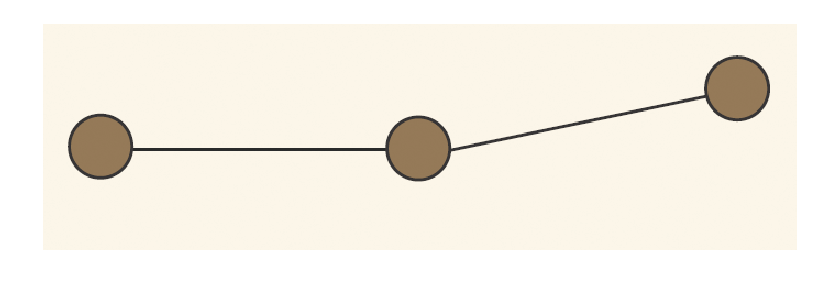
\includegraphics[width=0.5\linewidth]{spho_book_TYS_images/2015q3.png}
	\caption{Dancing coins}
\end{figure}

\subsection{Question 4}
4. Down the helix \\
A long helix is made of a thin metal wire. The axis of the helix is vertical. The radius of the loop of the helix is $r$, and the distance between the adjacent loops is $d$. A small bead begins to slide down the helix. Eventually, the bead reaches a constant speed $v$. Find the coefficient of the kinetic friction $k$ between the bead and the helix. 

\begin{figure}
	\centering
	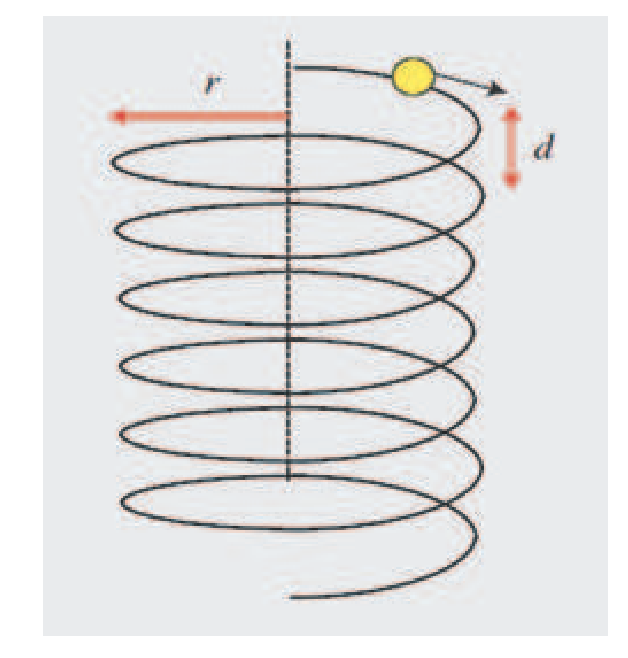
\includegraphics[width=0.5\linewidth]{spho_book_TYS_images/2015q4.png}
	\caption{Helix}
\end{figure}

\subsection{Question 5}
5. Flywheel \\
A $100 \mathrm{~m}^{2}$ solar panel is coupled to a flywheel such that it converts incident sunlight into mechanical energy of rotation with efficiency of $1 \%$. \\
(a) With what angular velocity would a solid cylindrical flywheel of mass $500 \mathrm{~kg}$ and radius $50 \mathrm{~cm}$ be rotating (if it started from rest)at the end of 8 hours of the solar panel? The solar constant is $8.4 \mathrm{~J} / \mathrm{cm}^{2} / \mathrm{min}$, for the full interval. \\
(b) Suppose the flywheel, whose axle is horizontal, were suddenly released from its stationary bearings and allowed to start rolling along a horizontal surface with kinetic coefficient of friction $\mu=0.1$. How far will it roll before it stops slipping? \\
(c) What speed is the center of mass moving at that moment? \\
(d) How much energy was dissipated as heat? [15] \\

\subsection{Question 6}
6. Human legs \\
Human legs are such that a person of typical size finds it comfortable to walk at a natural, swinging pace of about one step per second, but uncomfortable to force a pace substantially faster or slower. Neglecting the effect of the knee joint, use the simplest model of considering a human leg to be a uniform pole of length $l$ to estimate the frequency which determines this pace. The gravitational acceleration is taken as $g$. [5] 

\subsection{Question 7} 
7. TV antenna \\ The lead-in wires from a television antenna are often constructed in the form of two parallel wires. Ignoring any magnetic flux inside the wires, express the inductance of a length of $x$ of this type of lead-in in terms of $x, w$ and $a$ where $a$ is the radius of the wires and $w$ is their center-to-center separation. [5]

\begin{figure}
	\centering
	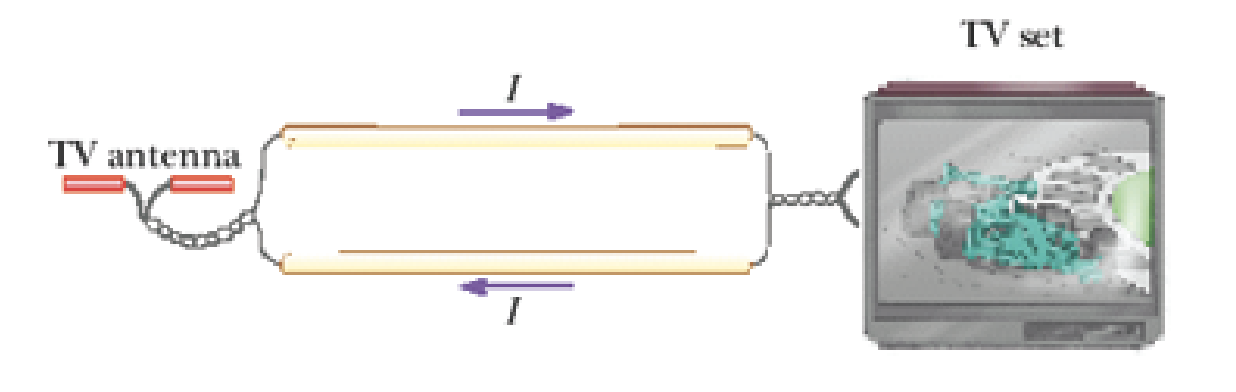
\includegraphics[width=0.5\linewidth]{spho_book_TYS_images/2015q7.png}
	\caption{TV set and antenna}
\end{figure}

\subsection{Question 8}
8. Star lifetime \\
A newly formed star consists almost entirely of hydrogen, which is converted to helium near the star's center by the following nuclear fusion reaction:
$$
4\left({ }_{1}^{1} p\right) \rightarrow_{2}^{4} H e+2 \beta^{+}+2 \nu
$$
In this equation, $\beta^{+}$represents a positron which is a particle of mass $0.000548 \mathrm{u}$ and charge $1.602 \times 10^{-19} \mathrm{C}$, and $\nu$ is a neutrino, which has no mass or charge. The mass of a proton is $1.007276 \mathrm{u}$, and the mass of a helium nucleus is $4.002604 \mathrm{u}$. \\
(i) Explain (in less than 25 words) why energy is released by this reaction, and calculate the total energy released by the fusion of $1 \mathrm{~kg}$ of hydrogen. [3] \\
(ii) Calculate the rate at which the Sun's mass is decreasing, given that the total solar power per unit area in the vicinity of the Earth is $1.4 \mathrm{kWm}^{-2}$, the Sun's mass is $2.0 \times 10^{30} \mathrm{~kg}$ and the period of the Earth's orbit about the Sun is $3.2 \times 10^{7} \mathrm{~s}$. [7] \\
(iii) Theory predicts that a star reaches the end of its life when about $10 \%$ of its mass has been converted from hydrogen into helium. Estimate the lifetime (in years) of the Sun. [2]

\subsection{Question 9}
9. Estimating the Earth's radius from the wake of a ship \\
If the Earth is flat and the horizon is infinitely far away, the parallel edges of a long straight wake (see figure below) would appear to converge to a point on the horizon. The Earth being round would result in the width of the wake being non-zero because the surface of the Earth will fall below the horizontal tangent plane of the observer.

\begin{figure}
	\centering
	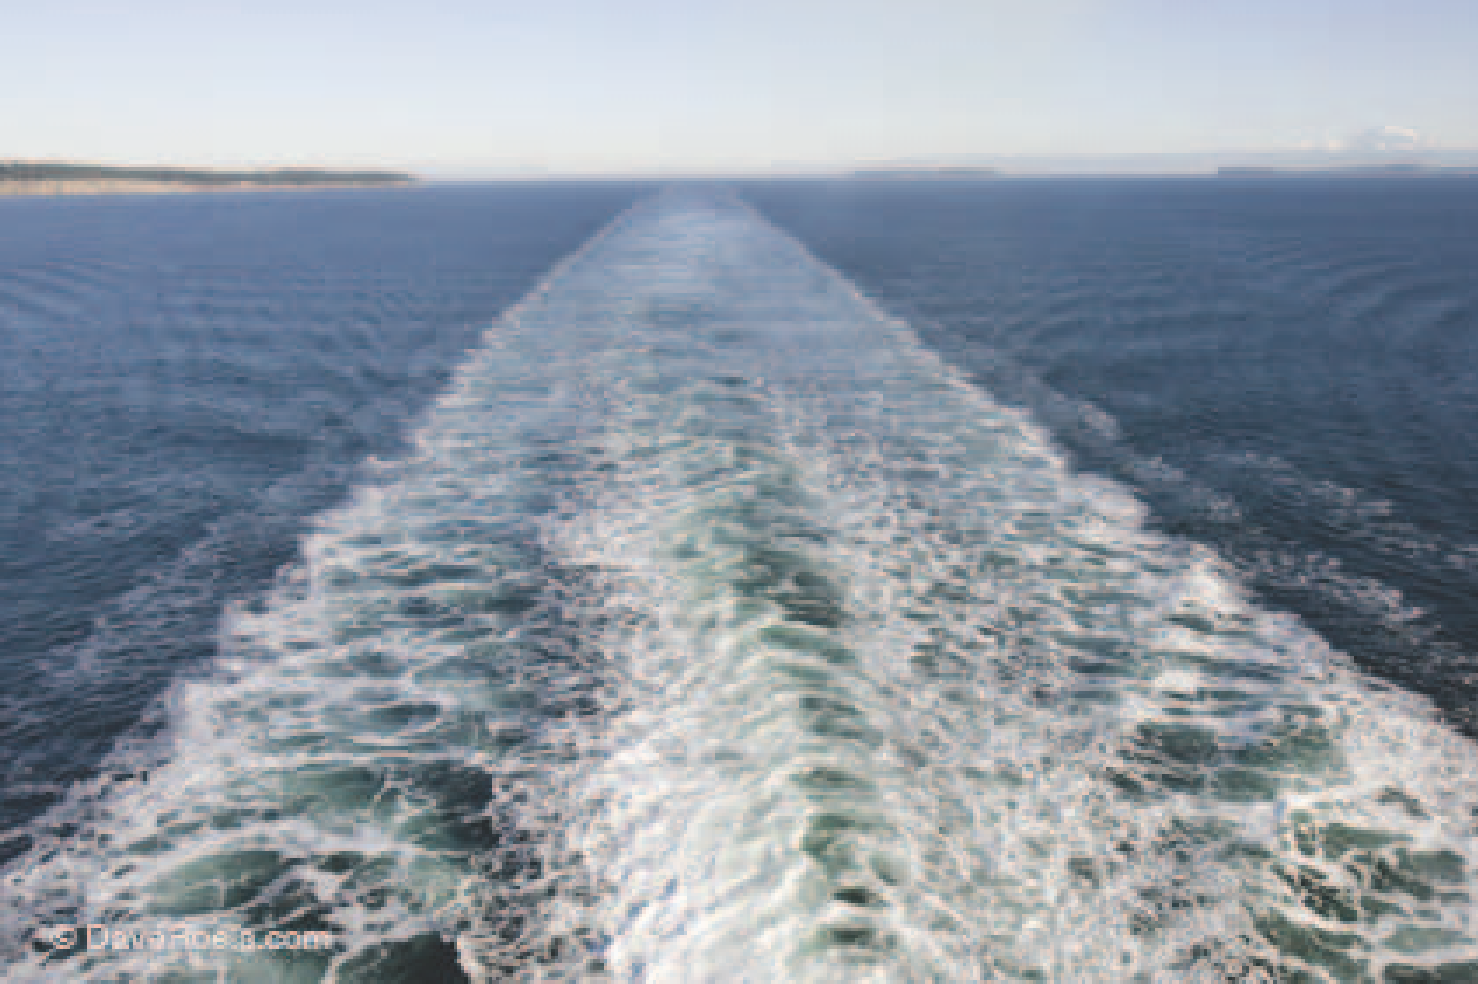
\includegraphics[width=0.5\linewidth]{spho_book_TYS_images/2015q9.png}
	\caption{Wake of a ship}
\end{figure}
Suppose the observer is at a height $h$, above the surface of the Earth. $\omega$ is the angle subtended at the observer's eyes by the width of the wake at the horizon and $W$ is the width of the wake. It is also helpful to define $D_{t}$, the distance to the horizon as seen by the observer. \\
(a) Express $\omega$ in terms of the other given variables. \\
(b) Express $R$, the radius of the Earth in terms of $\omega, W, h$ and other relevant constants. \\
(c) If $h$ is measured to be $32 \mathrm{~m}$ and $\omega$ is measured to be $4.6$ minutes of arc (recall that there are sixty minutes of arc in one degree), what would be the radius of the Earth as calculated from this technique? [2]

\subsection{Question 10}
10. Total resistance \\
There are 2015 points on a giant circuit board. Each point is connected to each of the other points by a wire of resistance $R$. Find the resistance $R_{\text {total }}$ between any two points.  [4]

\subsection{Question 11}
11. Image of a charge \\
A point charge $q$ is placed in the vicinity of a grounded metallic sphere of radius $R$ (see figure (a) below), and consequently a surface charge distribution is induced on the sphere. To calculate the electric field and potential from the distribution of this induced surface charge is a formidable task. However, the calculation can be considerably simplified by using the so called method of images. In this method, the electric field and potential produced by the induced charge distributed on the sphere can be represented as an electric field and potential of a single point charge placed inside the sphere, as shown in figure(b) (you do not have to prove it). Note: The electric field of this image charge reproduces the electric field and the potential only outside the sphere (including its surface).

\begin{figure}
	\centering
	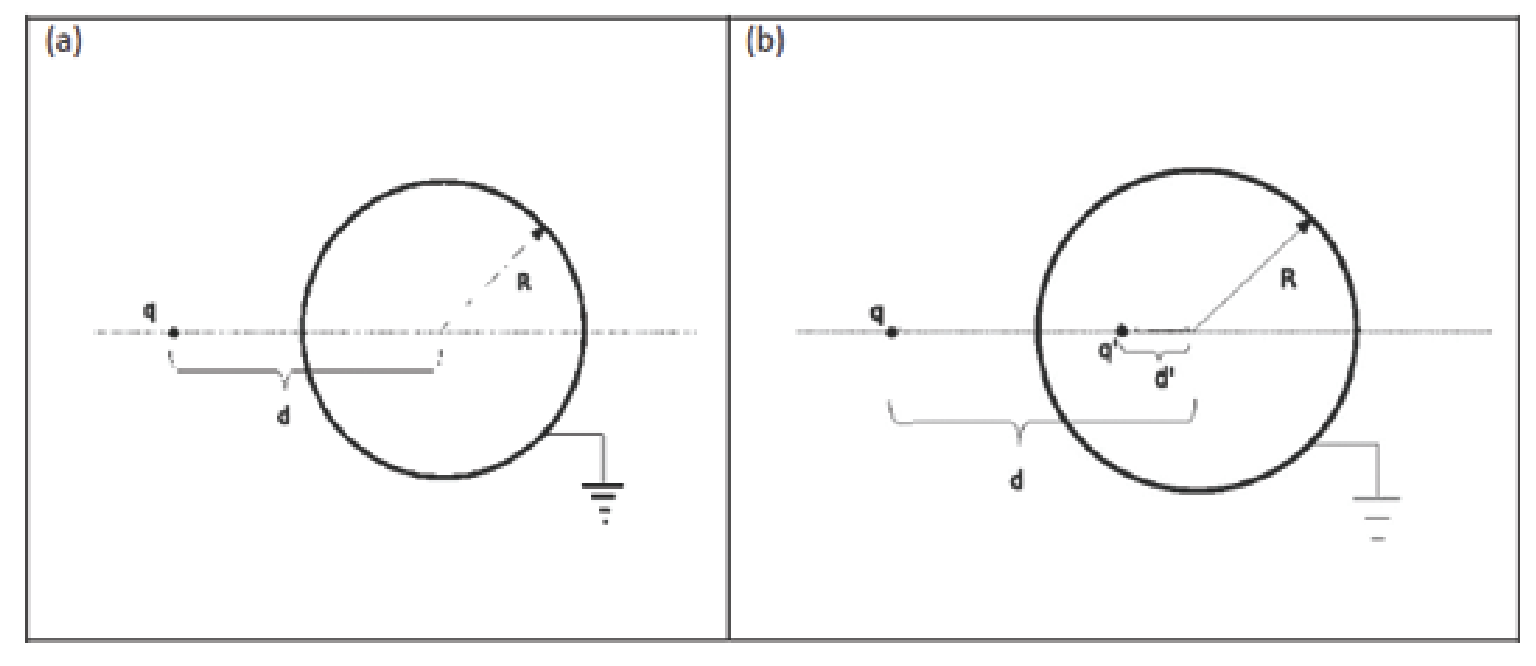
\includegraphics[width=0.5\linewidth]{spho_book_TYS_images/2015q11.png}
	\caption{
		Figure (a) A point charge $q$ in the vicinity of a grounded metallic sphere. \\
		Figure(b) The electric field of the charge induced on the sphere can be represented as the electric field of an image charge $q^{\prime}$. \\
		The symmetry of the problem dictates that the charge $q^{\prime}$ should be placed on the line connecting the point charge $q$ and the center of the sphere (see figure(b)).
	}
\end{figure}
(a) Write down the value of the electric potential on the sphere. [1] \\
(b) Express $q^{\prime}$ and the distance $d^{\prime}$ of the charge $q^{\prime}$ from the center of the sphere, in terms of $q, d$ and $R$. [9] \\
(c) Find the expression for the magnitude of the force acting on the charge $q$. Is this force repulsive? [2]

\section{2016}

\subsection{Question 1}
1. Hohmann transfer orbit and gravity assist

(a) A spacecraft is to be sent from Earth to Saturn. The Hohmann transfer is a manoeuvre that transfers the
spacecraft from Earth’s orbit around the Sun (assumed to be circular) to Saturn’s orbit around the Sun (assumed
to be circular also). This is done by pushing the spacescraft into an elliptical orbit that has its perihelion and
aphelion touching Earth’s orbit and Saturn’s orbit, respectively.

\begin{figure}
	\centering
	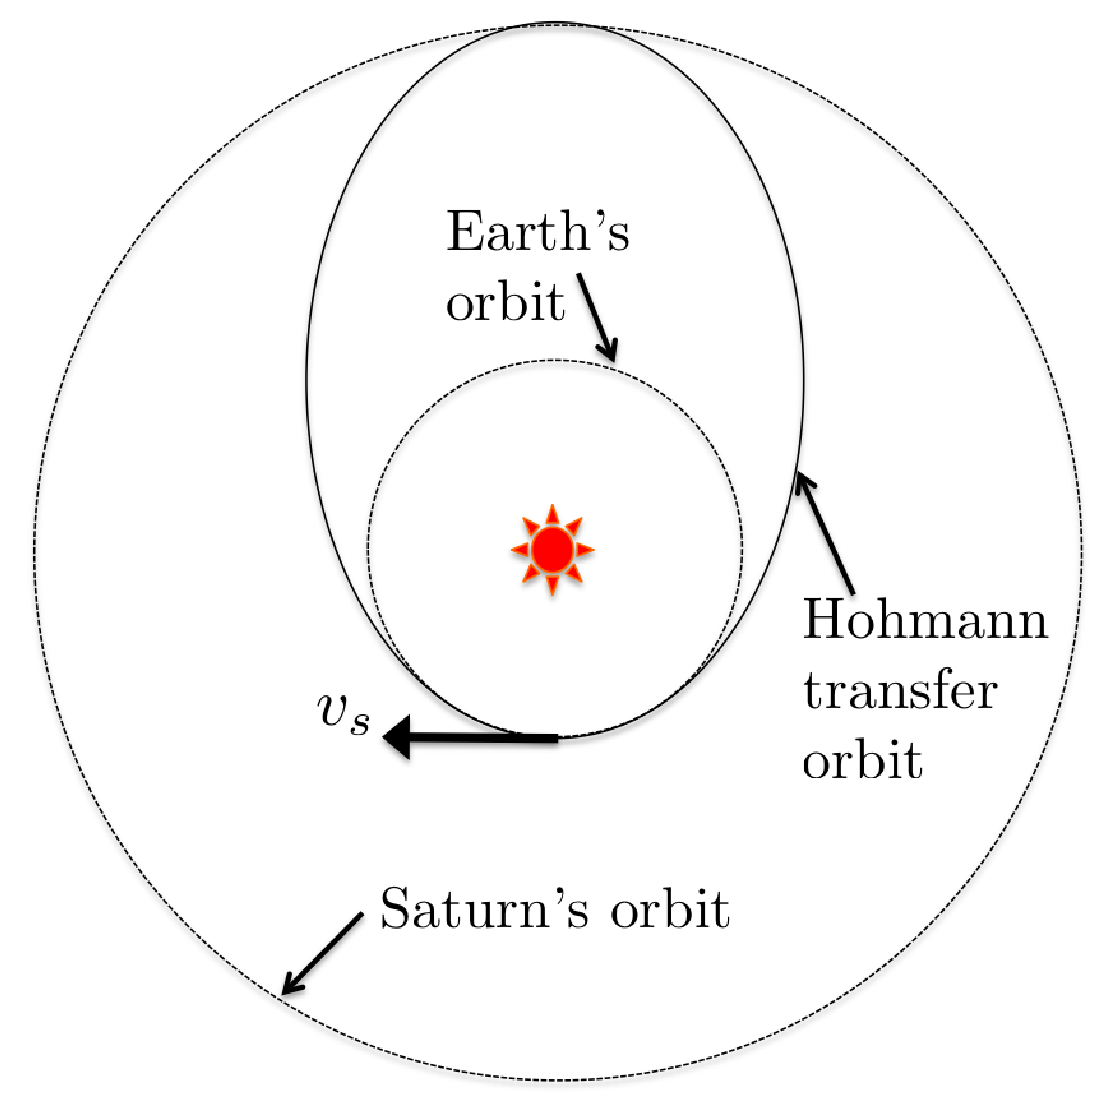
\includegraphics[width=0.5\linewidth]{spho_book_TYS_images/2016q1.png}
	\caption{Hohmann transfer orbit from Earth to Saturn. $v_s$, is the velocity of the spacecraft.}
\end{figure}

(i) Assuming that the spacecraft is initially travelling at the velocity of Earth around the Sun, calculate the change in velocity $\Delta v$ for the spacescraft to transfer from Earth's orbit to the elliptical orbit. Ignore the Earth's and Saturn's gravitational forces on the spacecraft. Use the constants below (and their corresponding symbols) in your working. [4 marks] \\
Earth's velocity around Sun: $v_{\oplus}=2.97 \times 10^{4} \mathrm{~m} / \mathrm{s}$ \\
Earth's orbital radius $r_{\oplus}=1.50 \times 10^{11} \mathrm{~m}$ \\
Saturn's orbital radius $r_{h}=1.43 \times 10^{12} \mathrm{~m}$ \\
Mass of Sun $M_{\odot}=1.99 \times 10^{30} \mathrm{~kg}$ \\
Gravitational constant $G=6.67 \times 10^{-11} \mathrm{Nm}^{2} / \mathrm{kg}^{2}$ \\
(ii) Calculate the time it takes for the spacecraft to travel from Earth's orbit to Saturn's orbit. [2 marks] \\
(b) The Cassini spacecraft was not sent to Saturn by a direct Hohmann transfer. Instead, it was first sent to Venus (via Hohmann transfer), where it gained speed, twice, using gravity assists by Venus. The first gravity assist by Venus changed the spacecraft's velocity and transferred the spacecraft to a more eccentric orbit, such that the spacecraft returned to its orbital perihelion after Venus had completed its orbit twice, and the spacecraft received the second gravity assist by Venus at that point. Calculate the change in velocity of the spacecraft during the first Venus' gravity assist. [6 marks]\\
Venus' orbital radius $r_{v}=1.08 \times 10^{11} \mathrm{~m}$ \\
Venus' orbital period $T_{v}=0.615$ years \\

\subsection{Question 2}
2. Consider a rigid axially symmetric wheel with mass $M$, moment of inertia $I$ about the axis of symmetry $S$, and radius $R$, moving in an upright position on a horizontal plane. The coefficient of kinetic friction between the wheel and the plane is $\mu_{k}$ \\
(a) The wheel is initially spun about $S$ with constant angular speed $\omega_{0}$, and is then released. It slips for a time $T_{a}$ and then rolls without slipping. Determine $T_{a}$ and the centre-of-mass speed $v_{a}$ of the rolling wheel. [4 marks] \\ 

\begin{figure}
	\centering
	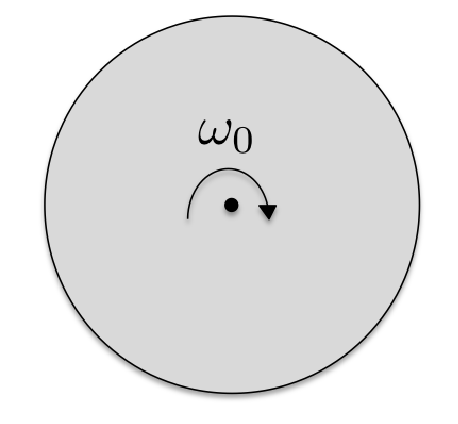
\includegraphics[width=0.5\linewidth]{spho_book_TYS_images/2016q2.png}
	\caption{Rolling wheel with initial angular speed $\omega_0$.}
\end{figure}

(b) The wheel has an initial horizontal centre-of-mass speed $v_{0}$ in addition to an initial angular speed $\omega_{0}$. Determine the time $T_{b}$ at which the wheel rolls without slipping and the centre of mass speed $v_{b}$ of the rolling wheel. [4 marks] 
\begin{figure}
	\centering
	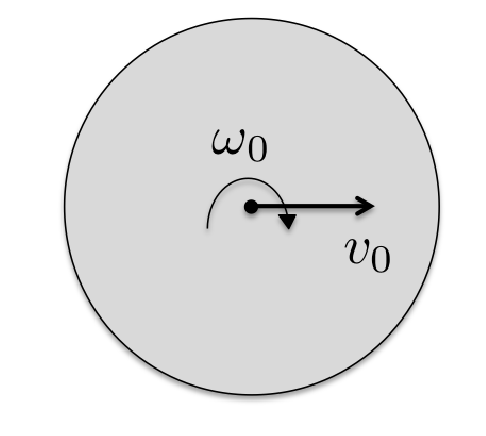
\includegraphics[width=0.5\linewidth]{spho_book_TYS_images/2016q2_2.png}
	\caption{Rolling wheel with initial angular speed $\omega_{0}$ and initial horizontal centre-of-mass speed $v_{0}$.}
\end{figure}

(c) The wheel has an initial horizontal centre of mass speed $v_{0}$ and an initial backspin $-\omega_{0}$. Determine the possible motions of the wheel. [4 marks]
\begin{figure}
	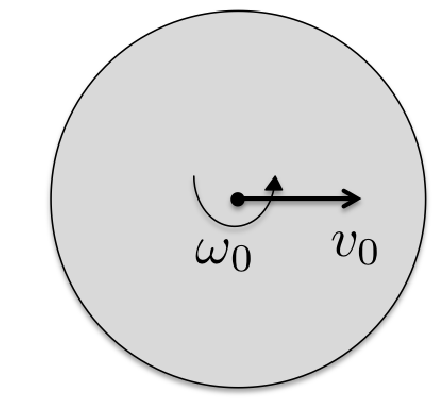
\includegraphics[width=0.5\linewidth]{spho_book_TYS_images/2016q2_3.png}
	\caption{Rolling wheel with initial backspin of angular speed $\omega_{0}$ and initial horizontal centre-of-mass speed $v_{0}$.}
\end{figure}

\subsection{Question 3}
3. A circular coil with radius $a$ is connected with an equilateral triangle on the inside as shown in the figure below. The resistance for each section of the wire is labeled. A uniform magnetic field $B(t)$ is pointing into the paper, perpendicular to the plane of the coil. $B(t)$ is decreasing over time at a constant rate $k .$ Given $2 r_{1}=3 r_{2} .$ Find $U_{A B}$, the potential difference between points $\mathrm{A}$ and $\mathrm{B}$. [10 marks]
\begin{figure}
	\centering
	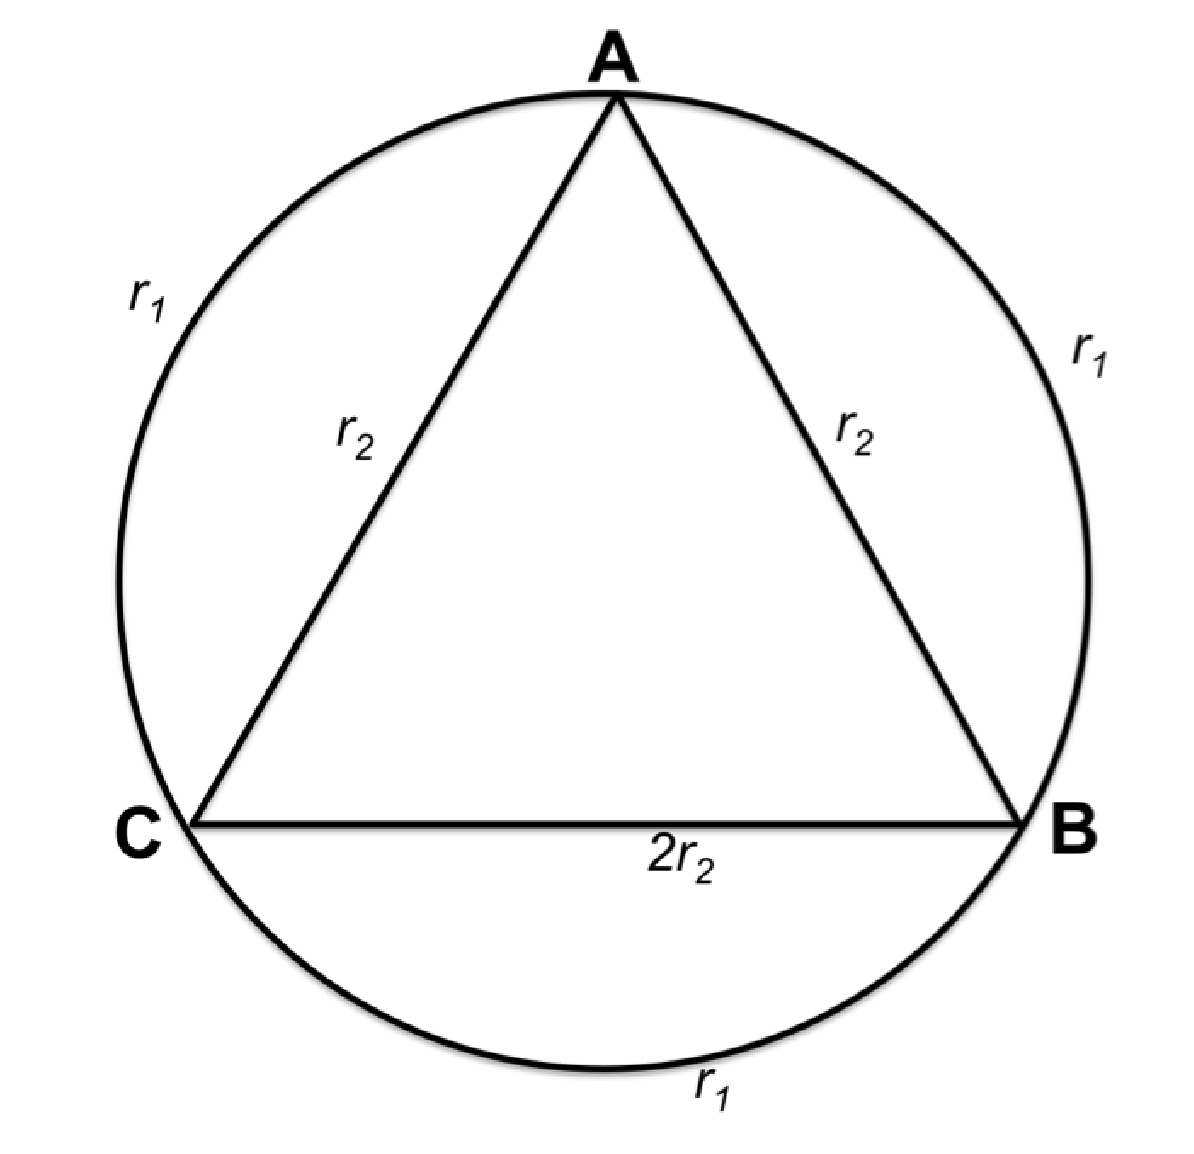
\includegraphics[width=0.5\linewidth]{spho_book_TYS_images/2016q3.png}
	\caption{Circular coil with 3 wires forming an equilateral triangle inside the circle.}
\end{figure}

\subsection{Question 4}
4. An experiment was performed to determine the value of the gravitational acceleration $g$ on Earth. Two equal masses of mass $M$ hang at rest from the ends of a string on each side of a light pulley (see figure below). A mass $m=0.01 M$ is placed on the right-hand-side mass. After the heavier side has moved down from rest by $h=1 \mathrm{~m}$ the small mass $m$ is removed. The system continues to move for the next $1 \mathrm{~s}$, covering a distance of $H=0.312 \mathrm{~m} .$ Find the value of $g$. [10 marks]
\begin{figure}
	\centering
	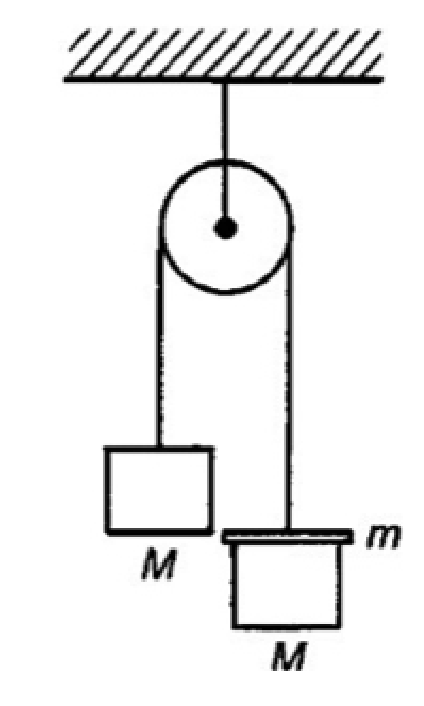
\includegraphics[width=0.5\linewidth]{spho_book_TYS_images/2016q4.png}
	\caption{Pulley with a system of masses attached.}
\end{figure}

\subsection{Question 5}
5. Consider the following decay
$$
{ }^{228} \mathrm{Th} \rightarrow{ }^{224} \mathrm{Ra}+\alpha
$$
The available energy $Q$ is given by
$$
Q=\left(m_{\mathrm{Th}}-m_{\mathrm{Ra}}-m_{\alpha}\right) c^{2}
$$
where $m_{\mathrm{Th}}, m_{\mathrm{Ra}}$, and $m_{\alpha}$ are the masses of Th-228, Ra-224 and the alpha particle respectively. \\
(a) Calculate the percentage of $Q$ carried by the alpha particle. [6 marks] \\
(b) In the above decay, the highest energy $\alpha$ particle has energy $5.423 \mathrm{~MeV}$ and the next highest energy is $5.341$ $\mathrm{MeV}$. Find the energy of the first excited state of Ra-224. [3 marks]

\subsection{Question 6}
6. We know that a rainbow can be formed by a ray entering a water droplet and exiting it after suffering a total internal reflection. We can call this a 'first-order' rainbow. The question is regarding the possibility of a 'zeroth' order rainbow where parallel rays impinging on a spherical raindrop is refracted into the drop and then out again into the air directly (without total internal reflection). \\
(a) Sketch a diagram depicting such a situation in a raindrop. Find the angle of deviation in terms of the angle of incidence $\theta_{i}$ and angle of refraction $\theta_{r}$. [2 marks] \\
(b) Show that the 'zeroth' order rainbow, given the above conditions, cannot exist. [3 marks] \\
In the following part of the question, we ask if a rainbow (or 'bubblebow') is able to be formed from the scattering of light in air bubbles in water. Again, we can consider parallel rays (i) entering the bubble and exiting without total internal reflection and (ii) entering and exiting with one (assumed) internal reflection at the gas-liquid interface. [3 marks] \\
(c) Sketch a diagram/s depicting the two situations in the bubble. Find the angle of deviation in each case. [3 marks]\\
(d) Work out if a rainbow (or 'bubblebow') can exist in each case. [4 marks] 

\subsection{Question 7}
7. Two infinitely long concentric hollow cylinders have radii $a$ and $4 a$. Both cylinders are insulators; the inner cylinder has a uniformly distributed charge per length of $+\lambda$; the outer cylinder has a uniformly distributed charge per length of $-\lambda$. \\
The inner cylinder is rotating clockwise about its axis with an angular velocity $\omega \ll c / a$, where $c$ is the speed of light. Assume that the permeability of the dielectric cylinder and the space between the cylinders is that of free space, $\mu_{0}$. \\
(a) Determine the electric field for all regions. [4 marks] \\
(b) Determine the magnetic field for all regions [4 marks] \\
(c) Determine the Poynting vector $\mathbf{S}=\frac{1}{\mu_{0}} \mathbf{E} \times \mathbf{B}$, for all regions. [2 marks]

\subsection{Question 8}
8. Consider a spaceship initially at rest in the lab frame. At a given instant, it starts to accelerate with constant proper acceleration $a$. Assume that the lab clock $(t)$ and spaceship clock $\left(t'\right)$ are synchronized such that this happens when $t=t'=0$. [Note: Proper acceleration is defined such that: at t'+dt', the spaceship is moving at speed a dt' relative to the frame it was in at time t'.] \\
(a) Determine the relative speed of the spaceship and the lab frame in terms of $t'$. Also, check the limit of the relative speed found when $a t' \ll c$ and comment. [5 marks] \\
(b) Find the relation between $t$ and $t'$ at later stage. Also, explore the relation for condition $a t' \gg c$. Comment. [5 marks] \\

\subsection{Question 9}
9. An electron bubble in liquid helium (adapted from APhO 2010 Taipei) \\
When an electron is planted inside liquid helium, it can repel the atoms around it isotropically, thus forming a spherical surface, inside which contains nothing but the electron itself. This is known as an electron bubble. \\
\\
The components of an electron's position vector $\vec{q}=(x, y, z)$ and momentum vector $\vec{p}=\left(p_{x}, p_{y}, p_{z}\right)$ must obey Heisenberg's uncertainty relations $\Delta q_{i} \Delta p_{i} \geq h / 4 \pi$, where $h$ is the Planck constant. \\
Note that the uncertainty of a variable $f$, denoted by $\Delta f$ is given by
$$
\Delta f=\sqrt{\overline{f^{2}}-\bar{f}^{2}}
$$
where the overhead bar denotes the average (mean) of the quantity under it. \\
Consider an electron bubble in liquid helium with an equilibrium radius $R$. The electron of mass $m$ moves freely inside the bubble with kinetic energy $E_{K}$ and exerts a pressure $P_{e}$ on the inner side of the bubble-liquid interface. The pressure exerted by liquid helium on the outer side of the interface is $P_{\text {He }}$. The liquid is kept at a constant temperature close to $0 \mathrm{~K}$ and the surface tension $\sigma$ is given by $3.75 \times 10^{-4} \mathrm{Nm}^{-1}$.  \\
(a) Find a relation between $P_{\mathrm{He}}, P_{e}$ and $\sigma$. [2 marks] \\
(b) Find a relation between $E_{K}$ and $P_{e}$. [4 marks] \\
(c) Let $E_{0}$ be the smallest possible value of $E_{K}$ consistent with Heisenberg's uncertainty relations when the electron is inside the bubble of radius $R$. Estimate $E_{0}$ as a function of $R$. [4 marks] \\
(d) Let $R_{e}$ be the equilibrium radius of the bubble when $E_{K}=E_{0}$ and $P_{\mathrm{He}}=0 .$ Obtain an expression for $R_{e}$ and calculate its value. [2 marks]



\section{2017}
\subsection{Question 1}
1. A planet is in a circular orbit about a massive star of mass $M$. The star undergoes a spherically symmetric explosion where its outer envelope is ejected to a distance well beyond that of the planet's orbit. The remnant of the star has mass $M^{\prime}$ which is still much greater than the mass of the planet. Find the eccentricity of the new orbit of the planet. Assume that the mass loss is instantaneous and that the planet itself is unaffected by the explosion. [10]

\subsection{Question 2}
2. Fermat's principle of least time states that the path taken between two points by a ray of light is the path that can be traversed in the least time (which implies stationary optical path length with respect to variations in the path). \\
a) Sketch the path of a light ray travelling from point A to point B as labelled in the diagram below. [2] \\

\begin{figure}
	\centering
	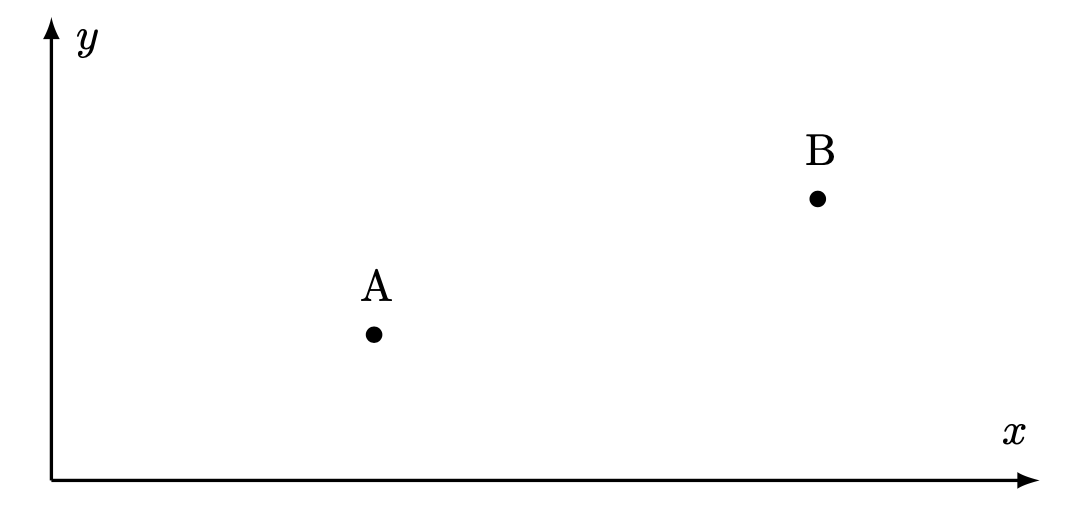
\includegraphics[width=0.5\linewidth]{spho_book_TYS_images/2017q2.png}
	\caption{}
\end{figure}
b) Consider a light ray that also departs from point $\mathrm{A}$, but reflects off the $x$-axis once at a point P before arriving at point B. Applying Fermat's principle to the trajectory APB, determine and sketch the path taken by the light ray. Comment on the angles made by the incident and reflected rays with respect to the surface normal at $P$. [4] \\
c) Now, consider a light ray travelling from point $\mathrm{A}$ to point $\mathrm{B}$ in two media with different indices of refraction, divided sharply by the $y$-axis as shown in the figure below. \\
\begin{figure}
	\centering
	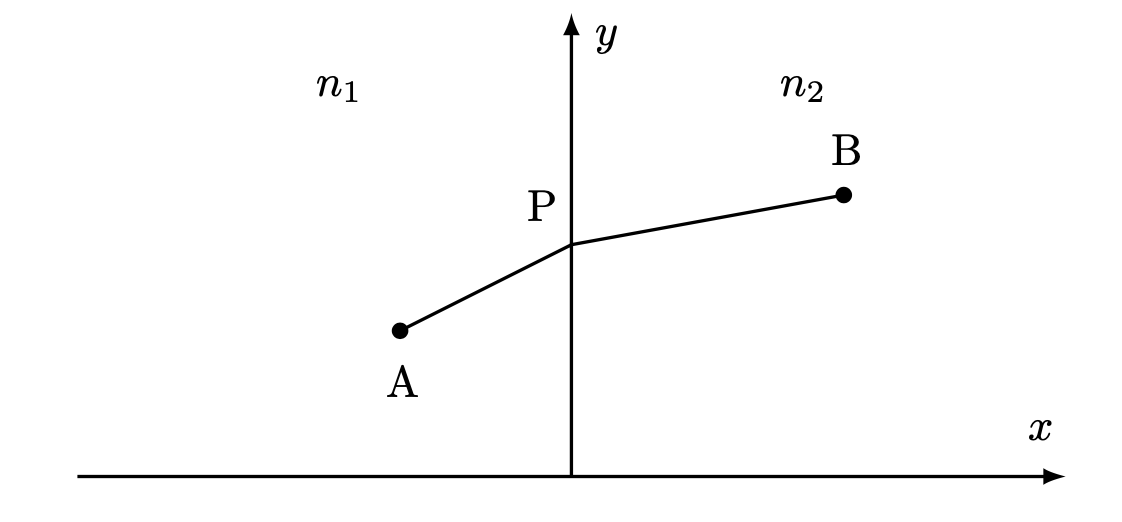
\includegraphics[width=0.5\linewidth]{spho_book_TYS_images/2017q2_2.png}
	\caption{}
\end{figure}
Point $\mathrm{A}$ is in a medium with refractive index $n_{1}$, while point $\mathrm{B}$ is in a medium with refractive index $n_{2}>n_{1}$. The light ray enters the second medium from the first via point P. Applying Fermat's principle to the trajectory APB, determine and sketch the path taken by the light ray. Comment on the angles made by the incident and refracted rays with respect to the surface normal at $\mathrm{P}$. [4]

\subsection{Question 3}
3. The chlorine radioisotope ${ }^{36} \mathrm{Cl}$ decays to ${ }^{36} \mathrm{Ar}$ with $98.1 \%$ probability and ${ }^{36} \mathrm{~S}$ with $1.9 \%$ probability. In a sample of old groundwater from a cave, the masses of ${ }^{36} \mathrm{Cl}$ and ${ }^{36} \mathrm{~S}$ were measured to be $20 \mu \mathrm{g}$ and $0.36 \mu \mathrm{g}$ respectively. The age of the sample was deduced to be $2.9 \times 10^{5}$ years old from the time of measurement. Calculate the half-life of ${ }^{36} \mathrm{Cl}$.

\subsection{Question 4}
4. An infinite ladder network of capacitors is connected to an $\mathrm{AC}$ voltage supply of $220 \mathrm{~V}$ and $50 \mathrm{~Hz}$ as shown below.
\begin{figure}
	\centering
	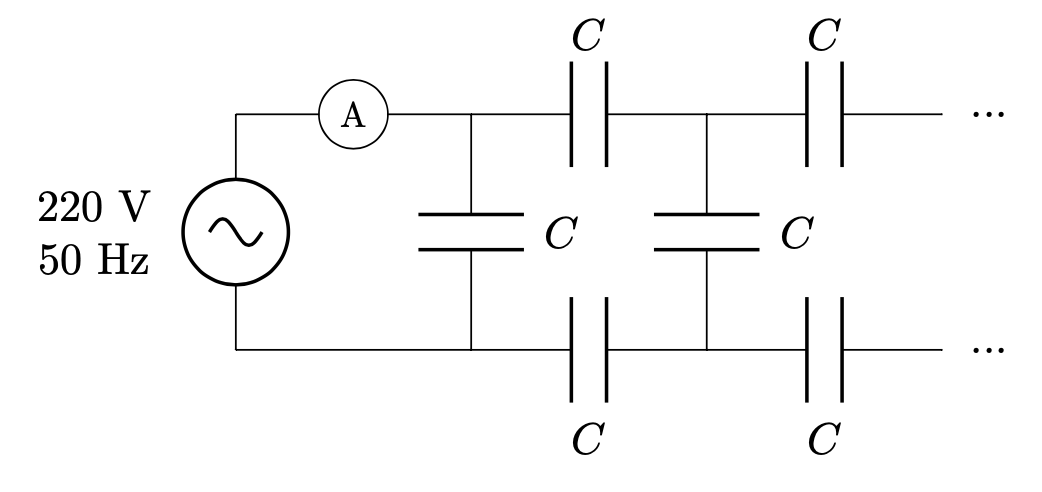
\includegraphics[width=0.5\linewidth]{spho_book_TYS_images/2017q4.png}
	\caption{}
\end{figure}
The capacitance of each capacitor is $1 \mu \mathrm{F}$. Find the current through the ideal $\mathrm{AC}$ ammeter to three significant figures.

\subsection{Question 5}
5. a) An inertial frame $S$ ' travels relative to another inertial frame $S$ with velocity $\beta c$ along the positive $x$-axis. Consider a photon of angular frequency $\omega$ and wavevector $\mathbf{k}$ in $S$. Evaluate the transformations of $\omega$ and $\mathbf{k}$ from $\mathrm{S}$ to $\mathrm{S}$ '. You may quote without proof that $\mathrm{K}^{\mu} \mathrm{X}_{\mu}$ is an invariant quantity, where $\mathrm{K}^{\mu}$ is the 4-wavevector and $\mathrm{X}^{\mu}$ is the 4-displacement. [5] \\
b) A plane mirror moves through vacuum with speed $\beta c$ in the $x$-direction. A beam of light with angular frequency $\omega_{i}$ is incident on the mirror at an angle $\theta_{i}$ to the normal as shown in the figure below. 
\begin{figure}
	\centering
	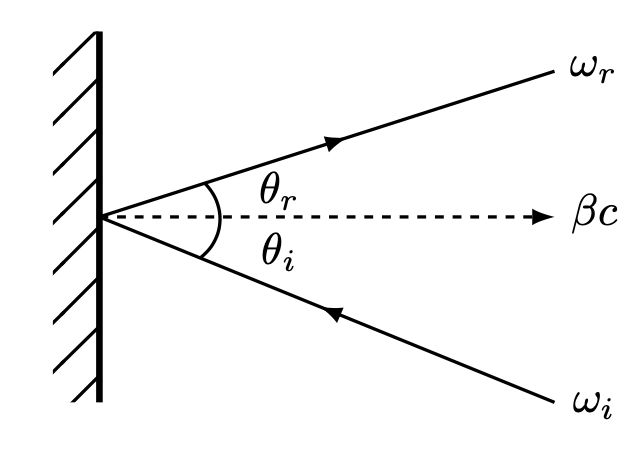
\includegraphics[width=0.5\linewidth]{spho_book_TYS_images/2017q5.png}
	\caption{}
\end{figure}
Determine the angular frequency $\omega_{r}$ and energy $E$ of each reflected photon. [5]


\subsection{Question 6}
6. Two identical balloons are inflated to different radii and connected via a thin tube. Contrary to conventional intuition, the smaller balloon deflates and the larger balloon inflates, instead of reaching an equal size. To explain this counter-intuitive result, we analyse the pressure-tension relation of stretching rubber. \\
a) The tension in a surface element of a stretched rubber balloon is
$$
F \propto \frac{r}{r_{0}^{2}}\left[1-\left(\frac{r_{0}}{r}\right)^{6}\right]
$$
where $r$ is the radius of the inflated balloon and $r_{0}$ is the original radius of the balloon. The figure below shows the tension acting on the surface element that arises from stretching the rubber, which acts tangential to the balloon.
\begin{figure}
	\centering
	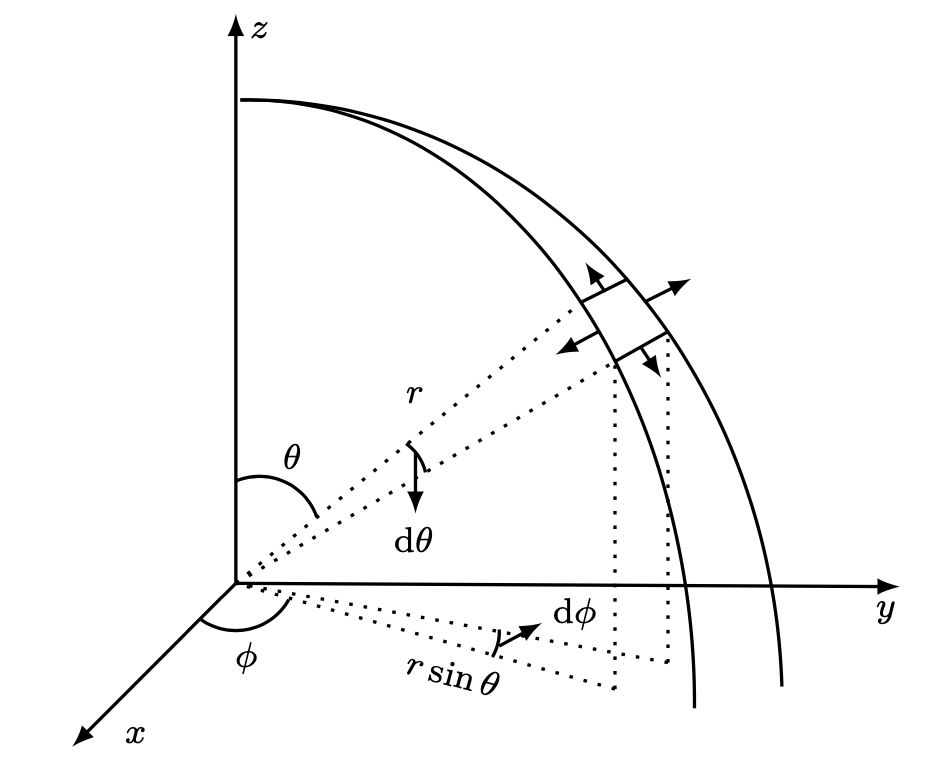
\includegraphics[width=0.5\linewidth]{spho_book_TYS_images/2017q6.png}
	\caption{}
\end{figure}
i) Show that the internal air pressure of the balloon, relative to the atmospheric pressure, is given by
$$
P=\frac{C}{r_{0}^{2} r}\left[1-\left(\frac{r_{0}}{r}\right)^{6}\right]
$$
where $C$ is a constant. [3] \\
ii) Show that the radius of the balloon at which the internal pressure is maximum is $r_{\max }=7^{\frac{1}{6}} r_{0}$. [1] \\
iii) Sketch the pressure-radius graph of the balloon. Label the points $r_{0}$ and $r_{\max }$ on your graph. [2] \\
b) Now, consider two balloons of two different radii connected via a thin tube. Initially, the smaller balloon is at its maximum radius, i.e. it has radius $r_{s_{i}}=7^{\frac{1}{6}} r_{0}$. After air is exchanged and the two balloons reach equilibrium, the final radius of the smaller balloon is $r_{s_{f}}=6^{\frac{1}{6}} r_{0}$. \\
i) Calculate the final radius of the bigger balloon $r_{b_{f}}$ at equilibrium as a multiple $r_{0}$ to three significant figures. You may use numerical methods to obtain your answer. [2] \\
ii) Calculate the initial radius of the bigger balloon $r_{b_{i}}$ as a multiple $r_{0}$ to three significant figures. You may use numerical methods to obtain your answer. You may use numerical methods to obtain your answer. [3] \\
iii) Suppose that the tube has cross-sectional area $A$, the average mass of an air molecule is $m$, and the experiment is conducted in a controlled environment of temperature $T$. Assuming that the tube is long and thin enough for the flow rate to be characterised by the r.m.s. speed of the particles constrained to a single dimension, show that the time taken for the two balloons to reach equilibrium is
$$
t \simeq \frac{16 \pi}{3 A} \sqrt{\frac{m}{k_{B} T}} \int_{r_{b_{i}}}^{r_{b_{f}}} \mathrm{~d} r_{b} \frac{r_{b}\left[1-2\left(\frac{r_{0}}{r_{b}}\right)^{6}\right]}{\frac{1}{r_{s}}\left[1-\left(\frac{r_{0}}{r_{s}}\right)^{6}\right]-\frac{1}{r_{b}}\left[1-\left(\frac{r_{0}}{r_{b}}\right)^{6}\right]}
$$
where $r_{s}$ and $r_{b}$ are the radii of the smaller and bigger balloons at a given instant respectively. [4]

7. a) Consider a volume $V$ bounded by a closed surface $\partial V$. There exist electrostatic fields $\mathbf{E}_{\text {in }}$ and $\mathbf{E}_{\text {out }}$ inside and outside $V$. Derive the boundary condition
$$
E_{\mathrm{out}}^{\perp}(\mathbf{r})-E_{\mathrm{in}}^{\perp}(\mathbf{r})=\frac{\sigma(\mathbf{r})}{\epsilon_{0}}
$$
where $\mathbf{r}$ is the position vector of any point along $\partial V, E^{\perp}(\mathbf{r})$ is the perpendicular component of $\mathbf{E}(\mathbf{r})$ to the surface at $\mathbf{r}, \sigma(\mathbf{r})$ is the surface charge density at $\mathbf{r}$, and $\epsilon_{0}$ is the permittivity of free space. [4] \\
b) Suppose $V$ is spherical and contains a continuous charge distribution with constant volume charge density $\rho$. Show that if $E_{\text {out }}\left(R^{-}\right)=E_{\text {in }}\left(R^{+}\right)$, then $\sigma$ is zero everywhere along $\partial V$. [5] \\
c) Suppose $V$ is a spherical conductor of radius $R$ and total charge $Q .$ If $V$ is cut into half, what is the repulsive force between the two halves? [6] 

\section{2018 (1.5h for Q1-5, 1.5h for Q6-9)}
\subsection{Question 1}
1. A particle $\mathrm{X}$ is projected with speed $v$ in a direction which makes an angle of $30^{\circ}$ from the horizontal. When this particle reaches the highest point of its trajectory, another particle $\mathrm{Y}$ is dropped from the roof of a tall building. The two particles collide at the base of the building. The particle $\mathrm{Y}$ takes a time of $0.17 \mathrm{~s}$ to fall a $5.0 \mathrm{~m}$ tall window in the building. The base of the window is $50.0 \mathrm{~m}$ above the ground. Ignore the effect of air resistance, find \\
i) the height of the building; [4] \\
ii) the value of $v$; [4] \\
iii) the distance of the point of projection of $X$ from the foot of the building. [2]

\subsection{Question 2}
2. A horizontal platform vibrates with simple harmonic motion in the horizontal direction with a period of $2.0 \mathrm{~s}$. A small object placed on the platform starts to slide when the amplitude of vibration reaches $0.4 \mathrm{~m}$. \\
i) Calculate the coefficient of static friction between the object and the platform. [5] \\
ii) The platform now excutes vertical simple harmonic motion with a period of $1.5 \mathrm{~s}$. What is the maximum amplitude of the motion if the object were to be in contact with the plate throughout the motion? [5]

\subsection{Question 3}
3. Consider a gas with molecular mass $m$ in a constant gravitational field $\mathbf{g}$. \\
i) Write down an equation relating a small change in pressure $\Delta P$ over a small change in height $\Delta z$. [1] \\
ii) Show that if the temperature $T$ is constant, the pressure of a gas $P(z)$ in a uniform gravitational field decreases with height $z$ according to the expression [9]
$$
P(z)=P(0) \mathrm{e}^{-\frac{m g z}{k_{B} T}}
$$

\subsection{Question 4}
4. A copper wire with mass $m$ is stretched between two fixed points at a distance $l$ apart. A tension $F_{T}$ is applied to the wire. When the copper wire is vibrating in the fundamental mode together with a $256 \mathrm{~Hz}$ tuning fork, a beat of frequency $5 \mathrm{~Hz}$ is observed. The copper wire is removed and a brass (which is an alloy made of copper and zinc) wire, with the same length and diameter, is stretched between the same two fixed points. The same tension is again applied to the brass wire. It is found that in this case, the brass wire, vibrating in the fundamental mode, resonates with the $256 \mathrm{~Hz}$ tuning fork when the two are vibrated together. [The mass densities of copper and zinc are $8940 \mathrm{~kg} \mathrm{~m}^{-3}$ and $7140 \mathrm{~kg} \mathrm{~m}^{-3}$ respectively.] \\
i) State an equation for the speed of the wave on the string in terms of $m, l$ and $F_{T}$ only. [1] \\
ii) Determine the percentage by mass of zinc in the brass wire. State any assumptions you make in your calculation. [9] 

\subsection{Question 5}
5. A $5.00 \mathrm{ml}$ solution was injected into the bloodstream of a patient. The solution contains radioactive iodine ${ }^{131} \mathrm{I}$ with a half-life of $8.025$ days at a concentration of $1.00 \times 10^{-10} \mathrm{~kg} \mathrm{~m}^{-3}$. The activity of a $5.00 \mathrm{ml}$ blood sample taken 24 hours later is found to be 3171 counts in 30 minutes. \\
i) Calculate the decay constant for ${ }^{131} \mathrm{I}$. [1]\\
ii) Calculate the total volume of blood in the patient's body given by these results. State any assumptions you make in your calculation. [9]

\subsection{Question 6}
6. A singly ionised helium atom, with electron in its ground state (i.e. principal quantum number $n=1)$, is at rest at position $\mathrm{O}$. A neutron of kinetic energy of $68.2 \mathrm{eV}$ is moving from the left (along the $x$-axis) towards $\mathrm{O}$ and collides inelastically with the helium atom. The neutron is scattered at an angle of $90^{\circ}$ relative to its original direction of motion (i.e. towards the $y$-axis). The helium atom, after the collision, is energetically excited and moves at an angle to the $x$-axis as shown below.

\begin{figure}
	\centering
	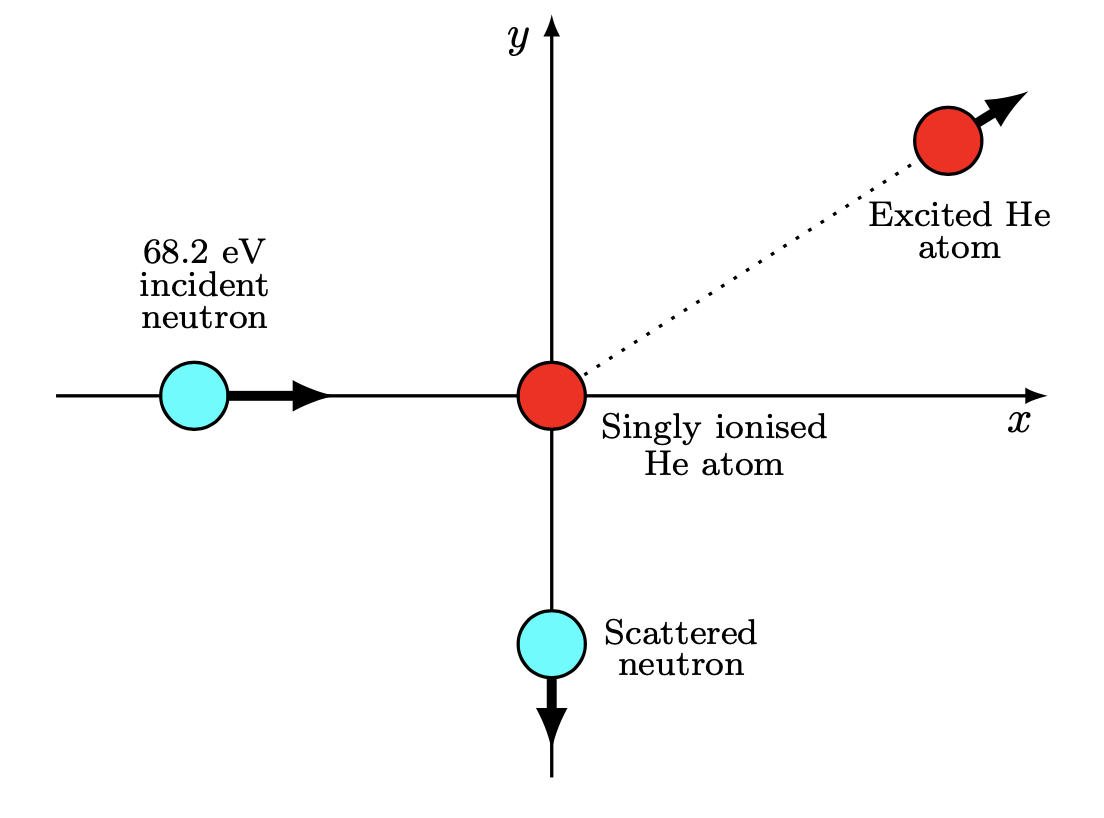
\includegraphics[width=0.5\linewidth]{spho_book_TYS_images/2018q6.png}
	\caption{}
\end{figure}

The mass of the helium atom is four times the mass of the neutron, and the energy levels of the helium atom are given by
$$
E_{n}=-\frac{54.4}{n^{2}} \mathrm{eV}
$$
i) Find the allowed values of the kinetic energies of the scattered neutron and helium atom after the collision. [8] \\
ii) If the helium atom de-excites subsequently by emitting radiation, find the range of wavelengths of the emitted radiation. For this part, you may assume that the momentum of the emitted photon is negligible. [4] \\
iii) When an atom emits a photon during a transition from the state with energy $E_{i}$ to the state with energy $E_{f}$, the energy of the photon is not exactly equal to the energy difference $E_{i}-E_{f}$. This is because the atom recoils, and part of the transition energy becomes the kinetic energy of recoil of the atom. Estimate the percentage of this energy difference that becomes the kinetic energy of the recoiling atom for the shortest wavelength case of the previous part. [2] \\
iv) Estimate the change in speed of the helium atom due to this transition. [2]

\subsection{Question 7}
7. A particle of mass $100 \mathrm{~g}$ is dropped from a height and falls vertically downward. The force due to air resistance is $-k v$, where $v$ is the speed of the particle and $k=1.09 \times 10^{-2} \mathrm{~kg} \mathrm{~s}^{-1}$ is a constant. \\
i) What is the terminal velocity of the particle? [1] \\
ii) How long does it take for the particle to achieve $99 \%$ of the terminal velocity? [4] \\
iii) How far has the particle fallen when it achieves $99 \%$ of the terminal velocity? [4]

\subsection{Question 8}
8. a) If a particle of charge $q$, mass $m$ and velocity $\mathbf{v}=v_{x} \hat{\mathbf{i}}+v_{y} \hat{\mathbf{j}}$ travels in a magnetic field $\mathbf{B}=B_{z} \hat{\mathbf{k}}$, then a Lorentz force $\mathbf{F}=F_{x} \hat{\mathbf{i}}+F_{y} \hat{\mathbf{j}}$ acts on the particle. As a result, the particle moves in a circular orbit. Assume that the particle is non-relativistic and that radiation is negligible. \\
i) Derive an expression for $T$, the time taken for the charged particle to make one complete revolution in the orbit in terms of $m, q$ and $B_{z}$. [2] \\
ii) Write down an expression for the acceleration of the particle $\mathbf{a}=a_{x}(t) \hat{\mathbf{i}}+a_{y}(t) \hat{\mathbf{j}}+a_{z}(t) \hat{\mathbf{k}}$ in terms of $v_{x}(t), v_{y}(t), v_{z}(t)$ and $T$. [3] \\
b) To compute the trajectory of the particle, we can estimate and compute the velocity of the particle after a short time step $\Delta t$, we can use a forward difference method. We assume that, to first-order, the acceleration in the $x$ and $y$-directions are constant during this short period of time such that $v_{x}(t+\Delta t) \simeq v_{x}(t)+a_{x}(t) \Delta t$ [3] \\
i) Write down the equations which determine $x(t+\Delta t)$ and $y(t+\Delta t)$ from $x(t)$ and $y(t)$ in terms of $T, B_{z}, q, m$ and $\Delta t$. [3] \\
ii) Derive an equation for the change in kinetic energy $\Delta E_{k}$ after time $\Delta t$ in terms of $T, B_{z}, q$, $m$ and $\Delta t$. [3] \\
iii) Calculate the ratio $E_{k_{f}} / E_{k_{i}}$ for $\Delta t=0.01 T$, where $E_{k_{i}}$ and $E_{k_{f}}$ are the kinetic energies at the start and end of an orbit respectively. [2]
c) Another method to compute the trajectory is to use a central difference method. We still assume that the acceleration in the $x$ and $y$-directions are constant during this short period of time $\Delta t$, but for $t>2 \Delta t$, when calculating the Lorentz force, we have instead
$$
v_{x}(t) \simeq \frac{x(t+\Delta t)-x(t-\Delta t)}{2 \Delta t} \text { and } a_{x}(t) \simeq \frac{x(t+\Delta t)-2 x(t)+x(t-\Delta t)}{\Delta t^{2}}
$$
i) Obtain equations to calculate $x(t+\Delta t)$ from $x(t)$ and $x(t-\Delta t)$, as well as $y(t+\Delta t)$ from $y(t)$ and $y(t-\Delta t)$, in terms of $B_{z}, q, m$ and $\Delta t$. [6] \\
ii) Derive an equation for the change in kinetic energy $\Delta E_{k}$ after time $\Delta t$ in terms of $B_{z}, q, m$ and $\Delta t$ via the central difference method. [4] \\
d) On the same diagram, sketch (alongside the actual trajectory of the particle) the trajectories of the particle as computed using the forward the central difference methods. [2]

\subsection{Question 9}
9. A rocket of proper length $600 \mathrm{~m}$ is moving directly away from the earth with uniform velocity. A radar pulse is sent out from the earth and is reflected from the reflectors at the back end and the front end of the rocket. The first reflected radar pulse is received back at the base $5.0$ minutes after emission and the second reflected pulse is received $12.0 \mu \mathrm{s}$ later. \\
i) Calculate the distance of the rocket from the earth at the instant the outgoing radar pulse hits the back end reflector. [2] \\
ii) Calculate the velocity of the rocket relative to the earth. [5] \\
iii) Calculate the time interval between the reflections at the back end and front end of the rocket measured in the inertial frame of the rocket. [3] \\
iv) Explain why the time interval between the reflections in the two frames (i.e. the earth frame and the rocket frame) are not related by the time dilation formula. [3]



\section{2019 (1.5h for Q1-5, 1.5h for Q6-10)}
\subsection{Question 1}
1. A projectile is fired with velocity $v_{0}$ at an angle $\theta$ to the horizontal. \\
i) The trajectory of the projectile intersects two points, both of which are at a height $h$ above the horizontal. Derive an expression for the horizontal distance $D$ between the two points. [7]  \\
ii) If the projectile is fired with an initial velocity of $200 \mathrm{~m} \mathrm{~s}^{-1}$, and the barrel of the gun is angled to achieve maximum range, calculate the value of $D$. [3]

\subsection{Question 2}
2. a) A $0.25 \mathrm{~kg}$ mass is attached to an unstretched spring with force constant $20 \mathrm{~N} \mathrm{~m}^{-1}$. The mass is released and oscillates with decaying amplitude, eventually coming to rest. The process is thermodynamically irreversible. Assuming that the temperature of the surroundings remains constant at $27^{\circ} \mathrm{C}$, calculate the change in entropy of the surroundings. [4] \\
bi) The intensity of sunlight reaching the surface of the Earth is $1.37 \times 10^{3} \mathrm{~W} \mathrm{~m}^{-1}$. Given that the radius of the Sun is $6.957 \times 10^{5} \mathrm{~km}$, and the orbital radius of the Earth about the Sun is $1.496 \times 10^{8} \mathrm{~km}$, estimate the surface temperature of the Sun. [3] \\
ii) Given that the orbital radius of Mars about the Sun is $2.280 \times 10^{8} \mathrm{~km}$, estimate the equilibrium temperature of Mars. [3]

\subsection{Question 3}
3. a) A particle of mass $0.1 \mathrm{~kg}$ oscillates in simple harmonic motion about a point $O$. The force acting on the particle is $F=-10 x \mathrm{~N}$, where $x$ is the displacement of the particle about $\mathrm{O}$. The particle begins at a distance of $0.05 \mathrm{~m}$ away from $\mathrm{O}$ with speed $\sqrt{3} / 2 \mathrm{~m} \mathrm{~s}^{-1}$. Calculate $\mathrm{i}$ ) the amplitude; ii) the initial phase; and iii) the maximum speed and acceleration of the particle. [4] \\
b) A rod of length $L$ and uniform cross-section is partially submerged vertically in a liquid, with a length $h<L$ exposed above the liquid. Show that the rod exhibits simple harmonic motion when given a small displacement, and derive an expression for the period of the motion. [6]

\subsection{Question 4}
4. a) The electric potential at the surface of a spherical oil droplet is $1000 \mathrm{~V}$. If two such droplets of equal charge and radius coalesce to form a single spherical droplet, what is the electric potential at the surface of the resulting droplet? You may assume charge is conserved. [5] \\
b) In a helium dilution refrigerator, ${ }^{3} \mathrm{He}$ and ${ }^{4} \mathrm{He}$ are mixed in a special chamber to obtain extremely low temperatures. The isotopes are sent through a Bainbridge mass spectrometer. \\
i) The strengths of the electric and magnetic fields in the spectrometer are $100 \mathrm{~V} \mathrm{~m}^{-1}$ and $0.2 \mathrm{~T}$ respectively. Calculate the speed of an ion which passes successfully through the velocity filter. [2] \\
ii) Deduce if the spectrometer can resolve the two isotopes if the exit slit of the velocity filter is $1 \mathrm{~mm}$ wide. [3]

\subsection{Question 5}
5. a) A beam of monochromatic light of intensity $50 \mathrm{~W} \mathrm{~m}^{-2}$ is incident normally onto a perfectly reflecting surface. Determine the pressure exerted on the surface. [5] \\
b) Positronium is a bound hydrogenic system with an electron orbiting a positron. The positron has the same mass as an electron, but carries a charge of $+|e|$ instead of $-|e| .$ Calculate the shortest wavelength of the Lyman series of the positronium system. [5]

\subsection{Question 6}
6. A projectile is fired with velocity $50 \mathrm{~m} \mathrm{~s}^{-1}$ from the edge of a cliff, which is at a height of $100 \mathrm{~m}$ above sea level. The projectile hits a target located at a horizontal distance of $300 \mathrm{~m}$ from the base of the cliff (which is at sea level). \\
i) Calculate the angle of inclination at which the projectile was fired. [4] \\
ii) Suppose that instead, at the instant the projectile was fired, the target begins to move away from the cliff at a constant speed of $10 \mathrm{~m} \mathrm{~s}^{-1}$. The angle of inclination remains the same as obtained in the previous part. Calculate the required initial speed of the projectile for it to hit the target. [5]

\subsection{Question 7}
7. a) A source $\mathrm{S}$ and a detector $\mathrm{D}$ are placed $120 \mathrm{~m}$ apart. S produces sound waves of wavelength $1.33 \mathrm{~m}$. A reflecting surface parallel to the line joining S and D is initially placed 90 $\mathrm{m}$ away as shown below.

\begin{figure}
	\centering
	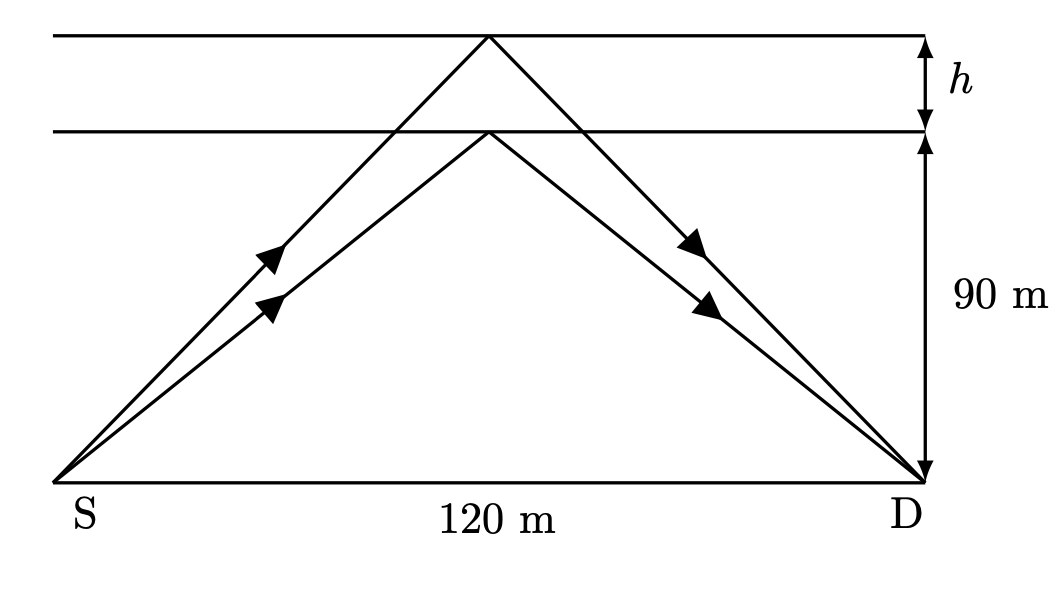
\includegraphics[width=0.5\linewidth]{spho_book_TYS_images/2019q7.png}
	\caption{}
\end{figure}

The sound waves directly from $\mathrm{S}$ and those reflected off the surface are found to be in phase at $\mathrm{D}$ and the intensity is at a maximum. The reflecting surface is then moved away from the line joining S and D by a distance $h$. How much should $h$ be for the intensity to be at the next maximum? [5] \\ 
b) A sonometer wire has diameter $0.51 \mathrm{~mm}$ and is made of a material of density $8.885 \times 10^{3}$ $\mathrm{kg} \mathrm{m}^{-3}$. It is stretched tightly over two bridges placed $60 \mathrm{~cm}$ apart. The tension in the wire is produced by hanging a uniform metal cylinder of diameter $5.0 \mathrm{~cm}$ and height $10.0 \mathrm{~cm}$ from the free end of the wire. The metal cylinder is slowly lowered into a liquid until half its volume is immersed. It is found that when the sonometer wire is vibrating in its second harmonic mode, the frequency of vibration is $118.4 \mathrm{~Hz}$. The metal cylinder is then completely immersed in the liquid. The new frequency of vibration of the second harmonic is $114.7 \mathrm{~Hz}$. Calculate the densities of the metal cylinder and the liquid. [7]

\subsection{Question 8}
8. a) A uniform hollowed sphere has inner and outer radii $r$ and $R$ respectively. Taking the gravitational potential at infinity to be zero, determine the ratio of the gravitational potential at the outer surface to that at the inner surface. [5] \\
bi) A uniform cylindrical copper rod of length $30.0 \mathrm{~cm}$ and diameter $2.0 \mathrm{~cm}$ is well-lagged such that the heat loss through the sides is negligible. One end of the rod is in thermal contact with a large heat reservoir maintained at temperature $200^{\circ} \mathrm{C}$, while the other is in thermal contact with another large heat reservoir maintained at $0^{\circ} \mathrm{C}$. Calculate the rate of change of entropy of the system. [The thermal conductivity of copper is $400 \mathrm{~W} \mathrm{~m}^{-1} \mathrm{~K}^{-1}$.] [3]  \\
ii) An electron, travelling at speed $2.08 \times 10^{6} \mathrm{~m} \mathrm{~s}^{-1}$, collides with a stationary hydrogen atom with orbital angular momentum $\hbar .$ Given that the energy levels of the hydrogen atom are
$$
E_{n}=-\frac{13.6}{n^{2}} \mathrm{eV} \text { for } n \in \mathbb{N}
$$
what are the possible wavelengths of the photons emitted by the hydrogen atom after the collision? [4] \\

\subsection{Question 9}
4. a) A negatively-charged particle of mass $m$ and charge $-q$ is placed at the centre of a uniformly charged ring of radius $a$ and linear charge density $\lambda$. The particle is constrained to move along the central axis of the ring, and is displaced by a distance $x \ll a$ along the axis. Given that the electric field along the central axis at a distance $x$ from the centre of a ring of radius $a$ and charge $Q$ is
$$
E=\frac{Q}{4 \pi \epsilon_{0}} \frac{x}{\left(a^{2}+x^{2}\right)^{\frac{3}{2}}}
$$
show that the particle exhibits simple harmonic motion, and determine the oscillation frequency. [6] \\
bi) In the Bohr model of the hydrogen atom, when the atom is in its ground state, the electron orbits the stationary proton with radius $5.3 \times 10^{-11} \mathrm{~m}$. The speed of the electron in the ground state orbit is $2.2 \times 10^{6} \mathrm{~m} \mathrm{~s}^{-1}$. Determine the magnitude of the magnetic field at the centre of the orbit due to the electron. [3] \\
ii) A circular disc of radius $R$ and surface charge density $\sigma$ spins at a rate of $n$ revolutions per second. Determine the magnetic field at the centre of the disc. [3]


\subsection{Question 10}
5. a) A particular event occurs at the origin of an inertial frame S at time $t=0$. Another event occurs at $x=4 \mathrm{~cm}, y=z=0$, and $t=5 \mathrm{~s}$ as measured in $\mathrm{S} .$ Determine the velocity of the inertial frame S', relative to S, in which the two events occur at the same point in space, as well as the time interval between the two events as measured by an observer in S'. [6] \\
b) A cube of side length $l$ and relativistic speed $u$ moves with one of its sides parallel to the $x$-axis of an inertial frame S. An observer moves along the $x$-axis of S with relativistic speed $v$. Derive an expression for the volume of the cube as measured by the observer. [6]



\section{2020}
\subsection{Question 1}
A cylindrical rod has a radius of 1.0 cm and length 1.0 m. It is made up of two sections, each of length 0.5 m. The material of one section is zinc and that of the other section is copper. The end of the rod made of zinc is pivoted to a fixed point O. The rod is first held so that it is horizontal and then released. Determine the angular velocity of the rod when it is in the vertical position. (Densities: zinc: 7135 kg $\text{m}^{-3}$; copper: 8940 kg $\text{m}^{-3}$) [10]

\subsection{Solution 1}
Mass of the zinc rod $m_{zinc} = \pi r^2 l \rho_{zinc} = \pi (0.01)^2 (0.50) (7135) = 1.1208 \text{ kg}$ \\
Mass of the copper rod $m_{copper} = \pi r^2 l \rho_{copper} = \pi (0.01)^2 (0.50) (8940) = 1.4043 \text{ kg}$ \\
\\ Moment of inertia about pivot 
\begin{align}
	&I=I_{zinc} + I_{copper}\\
	&=\frac{1}{3} m_{zinc} l^2 + \left(\frac{1}{12} m_{copper} l^2 + m_{copper} (1.5l)^2\right) \text{ (by parallel axis theorem)} \\
	&= \frac{1}{3} 1.1208 (0.5)^2 + \left(\frac{1}{12} 1.4043 (0.5)^2 + 1.4043 (1.5(0.5))^2\right) \\
	&= 0.91258 \text{ kg m}^2
\end{align}
By conservation of energy, (rotational) kinetic energy + gravitational potential energy should be conserved.
\begin{align}
	\frac{1}{2} I \omega^2 &= m_{zinc}g \Delta h_{zinc} + m_{copper}g \Delta h_{copper} \\
	\frac{1}{2}(0.91258) \omega^2 &= (1.1208)(9.81)(0.25) + (1.4043)(9.81)(0.75) \\
	\omega &= 5.3542 \text{ rad s}^{-1}
\end{align}

\subsection{Question 2}
(a) A student is sitting on a swing which is swinging back and forth with a constant angular amplitude of 45°. The length of the swing is 5 m. A loudspeaker, placed at a short distance away from the swing, produces a sound with a constant frequency of 400 Hz. What are the maximum and minimum frequency of the sound heard by the student? (Speed of sound waves = 330 m/s) [5] \\
(b) A compound microscope contains two thin lenses of focal length 6.0 mm and 40.0 mm respectively. The lenses are separated by a distance of 200 mm. The final image is formed 250 mm away from the eye lens. Calculate [5] \\
(i) The distance of the object from the objective lens \\
(ii) The magnifying power of the microscope\\
\subsection{Solution 2}
(a) The maximum doppler shift occurs when the swing is moving at its highest speed, i.e., at the lowest point. By the principle of conservatio nof energy,
\begin{align}
	\frac{1}{2} mv^2 &= mgl \left(1-\cos 45^\circ \right)\\
	\frac{1}{2} v^2 &= (9.81)(5) \left(1-\cos 45^\circ \right)\\
	v &= 5.3603 \text{ms}^{-1}
\end{align}
Hence,
\begin{align}
	f_{max} & = \frac{v_{sound}+v}{v_{sound}} f = \frac{330+5.3603}{330} \times 400 = 406.50 \text{ Hz} \\
	f_{min} & = \frac{v_{sound}-v}{v_{sound}} f = \frac{330-5.3603}{330} \times 400 = 393.50 \text{ Hz}
\end{align}
\begin{figure}
	\centering
	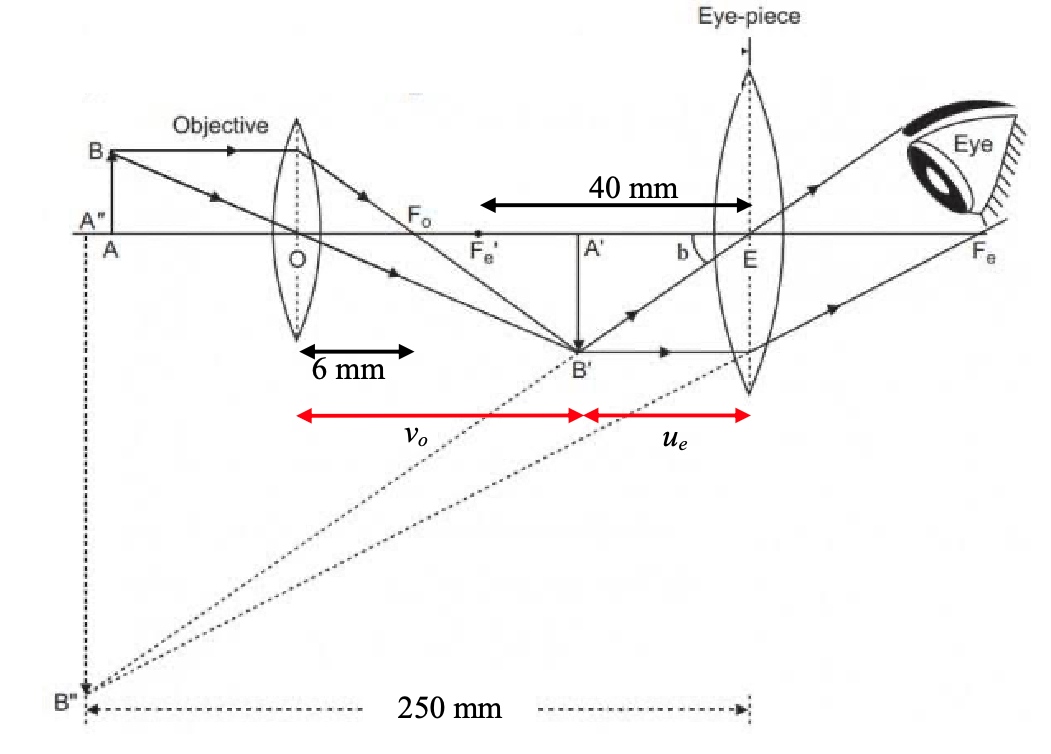
\includegraphics[width=\linewidth]{spho_book_TYS_images/2020q2.png}
\end{figure}
(b) 
\[f_o = 6 \text{ mm}\]
\[f_e = 40 \text{ mm} \quad v_e = -250 \text{ mm} \quad u_e = 200 - v_o \]
\begin{align}
	\frac{1}{u_e} + \frac{1}{v_e} &= \frac{1}{f_e} \\
	\Rightarrow	\frac{1}{200-v_o} + \frac{1}{-250} &= \frac{1}{40} \\
	\Rightarrow v_o &= 165.52 \text{ mm}
\end{align}
Hence,
\begin{align}
	\frac{1}{u_o} + \frac{1}{v_o} &= \frac{1}{f_o} \\
	\Rightarrow	\frac{1}{u_o} + \frac{1}{165.52} &= \frac{1}{6} \\
	\Rightarrow u_o &= 6.2257 \text{ mm}
\end{align}
\[u_e = 200-v_o = 200-165.52 = 34.480 \text{ mm}\]
Hence, magnification of eye lens $= \frac{250}{34.480} = 7.2506$ \\
And magnification of objective lens $ = \frac{165.52}{6.2257} = 26.587$ \\
Combined power of microscope $= 7.2506 \times 26.587 = 192.77 $
\subsection{Question 3}
One end of a thin conducting rod of length $l$ is pivoted to a fixed point. The rod has a resistance of $R$ and its two ends of the rod are connected to a resistor with resistance $R_0$. The rod is rotating with a constant angular velocity $\omega$ in a uniform magnetic field of flux density $B$. This direction of magnetic field is normal to the plane of rotation of the rod. [10]\\
(a) What is the emf induced in the rod? \\
(b) Determine the electric power developed in the resistor. \\
(c) Describe, with evidence, the origin of the electric power developed in the resistor.

\subsection{Solution 3}
3 (a) Induced emf $=B l v$
$$
=B l\left(\frac{1}{2} l \omega\right)
$$
$$
=\frac{1}{2} B l^{2} \omega
$$
(b) Power $=\frac{V^{2}\left(\frac{R_{o}}{R+R_{o}}\right)^{2}}{R_{o}}=\frac{\frac{1}{4} B^{2} l^{4} \omega^{2} R_{o}}{\left(R+R_{o}\right)^{2}}$ \\
(c) The electric power comes from the mechanical power input to sustain the circular motion of the rod which experiences an opposing torque due to the induced current.
The total electrical power dissipated is $=\frac{V^{2}}{R+R_{o}}=\frac{\frac{1}{4} B^{2} l^{4} \omega^{2}}{R+R_{o}}$
The induced current is $\frac{V}{R+R_{o}}=\frac{\frac{1}{2} B l^{2} \omega}{R+R_{o}}$
For each short length $d x$ of the rod located $x$ from the pivot, the torque is
$$
d \tau=x \cdot(B I d x)=B\left(\frac{\frac{1}{2} B l^{2} \omega}{R+R_{o}}\right) x d x=\frac{1}{2} \frac{B^{2} l^{2} \omega}{R+R_{o}} x d x
$$
Hence, total torque is
$$
\tau=\frac{1}{2} \frac{B^{2} l^{2} \omega}{R+R_{o}} \int_{0}^{l} x d x=\frac{1}{2} \frac{B^{2} l^{2} \omega}{R+R_{o}}\left(\frac{l^{2}}{2}\right)=\frac{1}{4} \frac{B^{2} l^{4} \omega}{R+R_{o}}
$$
Total mechanical power $=\tau \omega=\frac{1}{4} \frac{B^{2} l^{4} \omega^{2}}{R+R_{o}}$ which is identical to the electrical power developed.

\subsection{Question 4}
A free electron collides with a hydrogen atom which is in the ground state. After the collision, the hydrogen atom is excited and during the process of de-excitation, two photons are emitted. The wavelength of one of the photons emitted is 656.3 nm. The electron, after the collision, has de Broglie wavelength of 1.915 nm. [10] \\
(a) What is the wavelength of the other photon emitted during the de-excitation? \\
(b)What is the speed of the free electron before collision?

\subsection{Solution 4}
4 (a) The energy levels of the hydrogen atom are $E_{n}=-\frac{13.6}{n^{2}} \mathrm{eV}$. The photon of $\lambda=$ $656.3 \mathrm{~nm}$ is due to the transition from $n=3$ to $n=2$ as can be verified as follows: $\quad \frac{h c}{\lambda}=E_{3}-E_{2}=-13.6 \times\left(1.6 \times 10^{-19}\right)\left(\frac{1}{3^{2}}-\frac{1}{2^{2}}\right)=3.022 \times 10^{-19} \mathrm{~J}$ $\Rightarrow \quad \lambda=\frac{6.63 \times 10^{-34} \times 299792458}{3.022 \times 10^{-19}}=6.58 \times 10^{-7} \mathrm{~m}$ which is almost the same as the given value.
Hence, the other photon is emitted when the hydrogen atom de-excites from $n=2$ to $n=1$.
$$
\begin{gathered}
	\frac{h c}{\lambda}=E_{2}-E_{1}=-13.6 \times\left(1.6 \times 10^{-19}\right)\left(\frac{1}{2^{2}}-\frac{1}{1^{2}}\right)=1.632 \times 10^{-18} \mathrm{~J} \\
	\Rightarrow \quad \lambda=\frac{6.63 \times 10^{-34} \times 299792458}{1.632 \times 10^{-18}}=1.22 \times 10^{-7} \mathrm{~m}
\end{gathered}
$$
(b) Let the initial energy of the electron be $E$ and its energy loss when it collided with the hydrogen atom be $\Delta E$.
$$
\Delta E=13.6 \times\left(1.6 \times 10^{-19}\right) \times\left(\frac{1}{1^{2}}-\frac{1}{3^{2}}\right)=1.93 \times 10^{-18} \mathrm{~J}
$$
The momentum $p$ of the electron after collision is 
$$
p = \frac{h}{\lambda} = 3.4621 \times 10^{-25} 
$$
Hence, $E=1.93 \times 10^{-18} + \frac{p^2}{2m} = 1.9958 \times 10^{-18}$
$$
\begin{aligned}
	&\frac{1}{2} m v^{2}= 1.9958 \times 10^{-18} \\
	&v=2.09 \times 10^{6} \mathrm{~m} \mathrm{~s}^{-1}
\end{aligned}
$$
Since $v \ll c$, we are justified in neglecting relativistic effects.


\subsection{Question 5}
(a) An airplane flying horizontally with a constant speed of $540 \text{km h}^{-1}$ at a height of $1200 \text{m}$ fires a projectile horizontally in its direction of motion at a speed of $u \text{ m s}^{-1}$ relative to the plane. At this instant, a vehicle is at a point on the ground d km horizontally from the airplane. The vehicle is moving with a constant speed of $40 \text{m s}^{-1}$ on a horizontal road in the direction of motion of the plane. What must be the minimum value of d so that the projectile will hit the vehicle? If, at the instant when the projectile is fired, the value of d is 5 times its minimum value, what is the speed of the projectile when it hits the vehicle? [7]\\
(b) A satellite is orbiting the Earth 400 km above the equator. Its sense of revolution follows the rotation of the Earth. When the satellite is vertically above a point P on the equator, it will take a photo of the region around P. How many photos can the satellite take in 24 hours? [5] 
\subsection{Solution 5}
5 (a) $540 \mathrm{~km} \mathrm{~h}^{-1}=\frac{540}{3.6}=150 \mathrm{~m} \mathrm{~s}^{-1}$
The time of flight can be calculated using $1200=\frac{1}{2} g t^{2} \Rightarrow t=15.64 \mathrm{~s}$
Hence, change in displacement $=(150+u-40) \times 15.64=1721+15.64 u$
To hit the vehicle, $d=1721+15.64 u$
For minimum $d$, set $u=0$. Hence,
$$
d_{\min }=\mathbf{1 7 2 1} \mathbf{m}
$$
If $d=5 d_{\min }=8603 \mathrm{~m}$,
$$
\begin{aligned}
	&8603=1721+15.64 u \\
	&u=440 \mathrm{~m} \mathrm{~s}^{-1}
\end{aligned}
$$
And speed of projectile $=\sqrt{(440+150)^{2}+(9.81 \times 15.64)^{2}}=\mathbf{6 1 0} \mathbf{~ m} \mathbf{s}^{-1}$
(b)
$$
\begin{aligned}
	m r \omega^{2} &=\frac{G M m}{r^{2}} \\
	\omega^{2} &=\frac{G M}{r^{2}} \cdot \frac{1}{r} \\
	&=g \cdot\left(\frac{R}{r}\right)^{2} \cdot \frac{1}{r} \\
	&=9.80\left(\frac{6371}{6371+400}\right)^{2} \cdot \frac{1}{(6371+400) \times 1000} \\
	\omega &=1.132 \times 10^{-3} \mathrm{rad} \mathrm{s}^{-1}
\end{aligned}
$$
Angular velocity of Earth's rotation is $\frac{2 \pi}{86400}=7.27 \times 10^{-5} \mathrm{rad} \mathrm{s}^{-1}$
Hence, relative angular velocity is $1.132 \times 10^{-3}-7.27 \times 10^{-5}=1.059 \times 10^{-3} \mathrm{rad} \mathrm{s}^{-1}$
Hence, $T=\frac{2 \pi}{\omega_{\text {rel }}}=5931 \mathrm{~s}$
Since there are $86400 \mathrm{~s}$ in one day, no of photos taken is $\frac{86400}{5931}=14.6$ photos. 

\subsection{Question 6}
(a) A charged insulating sphere of radius R has a uniform positive charge density $\rho$ throughout its entire volume. A very narrow tunnel is drilled along the sphere’s diameter passing through the centre of the sphere. A charged particle of mass m carrying a charge $-q$ is placed at one end of the tunnel and released. Describe the subsequent motion of the charged particle. What is the speed of the particle when it passes through the centre of the sphere? [6] \\
(b) A particle P of mass m moves along a straight line joining two fixed points A and B. The particle is under the action of two forces $F_A$ and $F_B$. $F_A$ acts towards the point A and has magnitude $2\mu m d_A$ where $d_A$ is the distance of the point P from A. $F_B$ acts towards the point B and has magnitude $\mu m d_B$ where $d_B$ is the distance of the point P from B. Given that $\mu$ is a constant, show that the motion of P is simple harmonic. Deduce an expression for the period of motion. During the oscillation, the particle is instantaneously at rest at the mid-point of AB. What is the amplitude of the oscillation and what is the kinetic energy of the particle when it is at O, the point where it experiences zero net force? [6]

\subsection{Solution 6}
6 (a) At a distance $r$ from the centre of the sphere, where $r \leq R$, the gravitational field strength is given by
$$
E=\frac{\left(\frac{4}{3} \pi r^{3} \rho\right)}{4 \pi \varepsilon_{o} r^{2}}=\left(\frac{\rho}{3 \varepsilon_{0}}\right) r
$$
Hence, the force acting the $-q$ is
$$
F=-q E=-\left(\frac{q \rho}{3 \varepsilon_{o}}\right) r
$$
The acceleration is thus $a=-\left(\frac{q \rho}{3 m \varepsilon_{o}}\right) r$
Since the term in the bracket consists of constants only, the acceleration of the charge is directly proportional to its displacement from the centre of the sphere and in opposite direction to the displacement. Hence, the charge $-q$ will oscillate in simple harmonic motion with angular frequency $\sqrt{\frac{q \rho}{3 m \varepsilon_{o}}}$ and amplitude $R$.
The speed at the centre is thus given by $v=\omega A=R \sqrt{\frac{q \rho}{3 m \varepsilon_{o}}}$.
(b) Let $d$ be the distance between $\mathrm{A}$ and $\mathrm{B}$.
$$
\begin{aligned}
	F_{\text {net }} &=F_{A}+F_{s} \\
	&=-2 \mu m d_{A}+\mu m\left(d-d_{A}\right) \\
	&=\mu m\left(d-3 d_{A}\right) \\
	&=-3 \mu m\left(d_{A}-d / 3\right) \\
	\Rightarrow a &=-3 \mu\left(d_{A}-d / 3\right)
\end{aligned}
$$
Therefore, the particle P oscillates about the point $d_{A}=1 / 3 d$ with $\omega=\sqrt{3 \mu}$.
The period is $T=\frac{2 \pi}{\omega}=\frac{2 \pi}{\sqrt{3 \mu}}$.
$$
\begin{aligned}
	&\text { Amplitude }=\frac{d}{2}-\frac{d}{3}=\frac{d}{6} \\
	&E_{k} \text { at } \mathrm{O}=\frac{1}{2} m \omega^{2} A^{2} \\
	&=\frac{1}{2}(3 m \mu)\left(\frac{d}{6}\right)^{2} \\
	&=\frac{m \mu d^{2}}{24}
\end{aligned}
$$

\subsection{Question 7}
(a) A container, the volume of which is $8.0\times 10^{-3} \text{ m}^3$, contains an ideal gas at a pressure of $1.14\times 10^5 \text{ Pa}$ and temperature $T$. The lid of the container is opened, causing the gas to expand adiabatically until its pressure $1.01\times 10^5 \text{ Pa}$. This results in a slight decrease in the mass of the gas in the container. The lid is then closed and the gas in the container is allowed to return to its initial temperature. Under the new equilibrium condition, the pressure of the gas is $1.06\times 10^5 \text{ Pa}$. [6] \\
(i) What will be the volume of the gas left in the container under the initial equilibrium condition; i.e. at pressure $1.14\times 10^5 \text{ Pa}$ and temperature $T$? \\
(ii) What is the value of $\gamma$, the ratio of the molar heat capacity of the gas at constant pressure to that at constant volume? \\
(iii) State, with reasons, what is the atomicity of the molecules of the gas? \\
(b) One end of a copper rod, with diameter 2.0 cm and length 50.0 cm, is in good thermal contact with a hot bath maintained at 100 °C while the other end is immersed in a mixture of 200 g ice and 100 g water initially maintained at 0 °C inside a container whose thermal capacity is negligible. Both the copper rod and the container are well-lagged. How long does it take for the temperature of the mixture to rise from 0 °C to 20°C? [6] \\
(Thermal conductivitiy of copper $= 400 \text{ W m}^{-1} \text{K}^{-1}$ \\ 
Specific heat capacity of water $=4200 \text{ J kg}^{-1} \text{K}^{-1} $ \\
Latent heat of fusion of water $= 3.34\times 10^5 \text{ J kg}^{-1}]$) 
\subsection{Solution 7}
7 (a) Imagine that the gas initially trapped in the container can be divided into the red portion and the blue portion below, and the blue portion escaped to the surrounding when the lid is opened and the gas expanded adiabatically. It is given that the final temperature of the remaining gas is $T$ and the pressure is $1.06 \times 10^{5} \mathrm{~Pa}$.
insert diagram
Hence, by $p V=n R T$ to diagrams 1 and 3 ,
$$
\frac{p_{f}}{p} \cdot \frac{V}{V}=\frac{n_{f}}{n} \cdot \frac{T}{T} \Rightarrow n_{f}=\frac{1.06}{1.14} n=0.930 n
$$
That is, $0.930$ of the original gas remains in the container.
(i) If this remaining gas is compressed to $1.14 \times 10^{5} \mathrm{~Pa}$ and remains at temperature $T$, then its volume is (using Boyle's Law):
$$
V_{f}=0.930 \times 8.0 \times 10^{-3}=7.44 \times 10^{-3} \mathrm{~m}^{3}
$$
(ii) Consider the adiabatic expansion of the "red gas", and applying $p V^{\gamma}=$ cosntant to diagrams 1 and 2 ,
$$
\begin{aligned}
	&\left(\frac{V}{V_{f}}\right)^{\gamma}=\frac{p_{f}}{p} \\
	\Rightarrow &\left(\frac{8.0}{7.44}\right)^{\gamma}=\frac{1.14}{1.01} \\
	\Rightarrow \quad & 1.075^{y}=1.129 \\
	\Rightarrow \quad & \gamma=1.67
\end{aligned}
$$
(iii) The molar heat capacity of a monatomic ideal gas at constant volume is $\frac{3 R}{2}$ while that at constant pressure is $\frac{5 R}{2}$. Hence, $\gamma=\frac{5 / 2}{3 / 2}=\frac{5}{3}=1.67$. That is, the atomicity of the gas molecules is 1 .
7 (b) The heat transfer can be broken down into two stages:
Stage 1 : when the ice is melting. The two ends of the copper rod are maintained at $100{ }^{\circ} \mathrm{C}$ and $0^{\circ} \mathrm{C}$ in this stage.
Stage 2: after the ice has fully melted, the cold water is gradually heated $\mathrm{up}$ to $20{ }^{\circ} \mathrm{C}$.
We will calculate the time taken for each stage as follows:
$\underline{\text { Stage } 1}$
$$
\begin{aligned}
	&\frac{d Q}{d t}=-k A \frac{d \theta}{d x}=-400 \times \pi(0.01)^{2} \times \frac{0-100}{0.500}=25.13 \mathrm{~W} \\
	&t_{1}=\frac{m_{i c e} l_{f}}{d Q / d t}=\frac{0.200 \times 3.34 \times 10^{4}}{25.13}=2658 \mathrm{~s}
\end{aligned}
$$
$\underline{\text { Stage } 2}$
$$
\begin{aligned}
	&\frac{d Q}{d t}=-0.04 \pi\left(\frac{\theta-100}{0.500}\right)=m c \frac{d \theta}{d t} \\
	&\Rightarrow \quad d t=\frac{0.500}{0.04 \pi} \times 0.300 \times 4200 \times \frac{d \theta}{100-\theta} \\
	&\Rightarrow \quad t_{2}=5013[\ln (100-\theta)]_{20}^{0}=1119 \mathrm{~s}
\end{aligned}
$$
Hence, total time taken $=2658+1119=3777 \approx \mathbf{3 7 8 0} \mathbf{s}$

\subsection{Question 8}
(a) Two identical sound sources A and B which emit sound waves with frequency 256 Hz are initially side by side together with a stationary observer. Source A remains stationary with respect to the observer, while source B accelerates from rest with a constant acceleration of 0.5 m s-2 until it reaches a point P. After this, B continues to move with a constant velocity that it attains at the point P. When this happens, the observer finds that the frequency of sound coming from source B differs from that from source A by 8 Hz. What is the distance of the point P from the observer? (Speed of sound waves in air = 330 m s-1) [5] \\
\begin{figure}
	\centering
	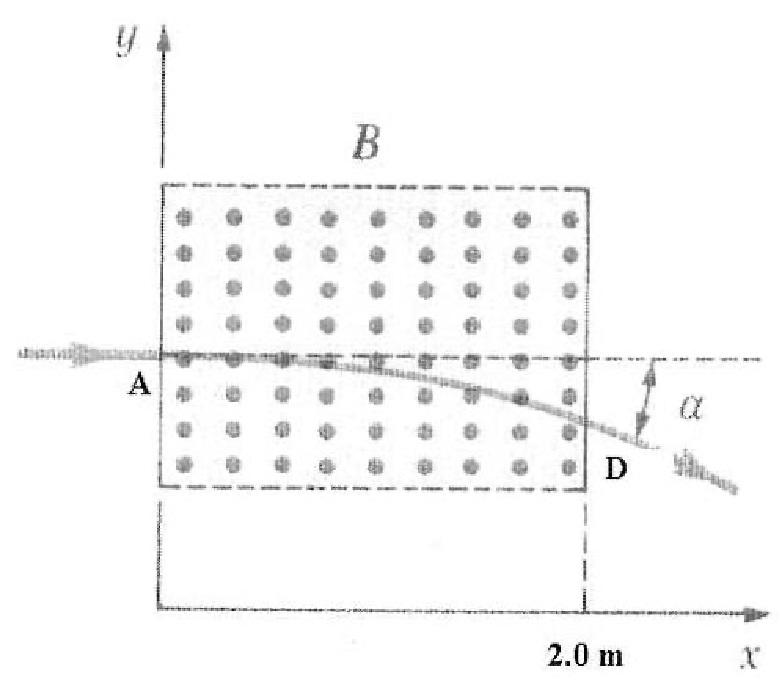
\includegraphics[width=\linewidth]{spho_book_TYS_images/2020q8}
\end{figure}
(b) A beam of protons with kinetic energy 10 MeV is travelling in the positive x-direction. It enters a magnetic field of magnitude 1.5 T and the direction of the magnetic field is the positive z-direction. The magnetic field extends from x = 0 to x = 2.0 m as shown in Fig. 1. Determine the angle $\alpha$ between the initial velocity vector of the proton bean and the velocity vector after the beam emerges from the magnetic field. [7] \\
\subsection{Solution 8}
8
(a) $f^{\prime}=f-8=248 \mathrm{~Hz}$
Hence, $248=256\left(\frac{c}{c+v}\right)$
$$
\begin{aligned}
	&31 c+31 v=32 c \\
	&v=\frac{1}{31} c=\frac{1}{31} \times 330=10.6 \mathrm{~m} \mathrm{~s}^{-1}
\end{aligned}
$$
By $v^{2}=u^{2}+2 a s$
$$
\begin{aligned}
	&10.6^{2}=2(0.5) s \\
	&s=\mathbf{1 1 3} \mathbf{m}
\end{aligned}
$$
(b) $\frac{1}{2} m v^{2}=1.6 \times 10^{-12} \Rightarrow v=\sqrt{\frac{1.6 \times 10^{-12} \times 2}{1.67 \times 10^{-27}}}=4.38 \times 10^{7} \mathrm{~m} \mathrm{~s}^{-1}$
Magnetic force provides the centripetal force:
$$
\begin{aligned}
	&\quad B q v=\frac{m v^{2}}{r} \\
	&\Rightarrow \quad r=\frac{m v}{B q}=\frac{1.67 \times 10^{-27} \times 4.38 \times 10^{7}}{1.5 \times 1.6 \times 10^{-19}}=0.305 \mathrm{~m}
\end{aligned}
$$
Therefore, since the radius of the trajectory of the proton is less than $2.0 \mathrm{~m}$, assuming that the magnetic field is of infinite extent in the $y$-direction (or more than $0.61 \mathrm{~m}$ from $\mathrm{A}$ in the negative $y$-direction), the proton will go through a semi-circular path before exiting the magnetic field again. Hence, $\alpha=180^{\circ}$.


\subsection{Question 9}
(a) Light with wavelength 122 nm is incident on the surface of a metal. The electrons, which are emitted with maximum kinetic energy, enters a magnetic field the direction of which is normal to the velocity vectors of these electrons. The flux density of the magnetic field is 5 x 10-5 T . These electrons are found to describe a circular path of radius 15.8 cm in the magnetic field. What is the work function of the metal? [5] \\
(b) Muons are particles which are created in the upper atmosphere via cosmic interactions. These particles travel vertically downward to the surface of the Earth at a speed of 0.995 c where c represents the speed of light in vacuum. When muons are at rest, they have a half-life of 1.56 $\mu$s. A muon counter is placed at the top of a mountain 2000 m high. The counter records 568 muons in 1 hour. \\
(i) According to classical concepts, what will be the number of muons counted in 1 hour if the counter is placed at the foot of the mountain? [2] \\
(ii) In a typical experiment, a counter placed at the foot of the mountain record 422 muons in 1 hour. Why does the result of this experiment differ so much from your result in part (i)? [2] \\
(iii) What is the “height” of the mountain according to muons? [1] \\
(iv) While the muons are travelling downward to the earth, another particle also travels in the same direction with speed 0.9995 c. What is the velocity of this particle in the muon’s inertial frame? [2]
\subsection{Solution 9}
9
$B q v=\frac{m v^{2}}{r}$ $\begin{aligned} \Rightarrow \quad r=\frac{m v}{B q} \\ 0.158 \end{aligned}=\frac{9.11 \times 10^{-31} \times v}{5 \times 10^{-5} \times 1.6 \times 10^{-19}}$ $v=1.39 \times 10^{6} \mathrm{~m} \mathrm{~s}^{-1}$ Hence, $K E_{\max }=\frac{1}{2} m v^{2}=8.77 \times 10^{-19} \mathrm{~J}$
$$
\begin{aligned}
	\text { Using } \frac{h c}{\lambda} &=\phi+K E_{\max }, \\
	\phi &=\frac{6.63 \times 10^{-34} \times 3.0 \times 10^{8}}{1.22 \times 10^{-7}}-8.77 \times 10^{-19}=7.53 \times 10^{-19} \mathrm{~J}
\end{aligned}
$$
(b) (i) Time taken to reach the ground level $=\frac{2000}{0.995 \times 3.0 \times 10^{8}}=6.70 \times 10^{-6} \mathrm{~s}$
$$
A=A_{o}\left(\frac{1}{2}\right)^{t / T_{V 2}}=568 \times\left(\frac{1}{2}\right)^{6.70 / .56}=29 \text { counts }
$$
(ii) This is due to time-dilation, i.e., in the reference frame of the muons, the time elapsed is $6.70 \times 10^{-6} / \gamma$, where $\gamma=(1-0.995)^{-1 / 2}=10.0$. So the time elapsed is $6.70 \times 10^{-7} \mathrm{~s}$ in the reference frame of the muons. The expected count rate should be
$$
A^{\prime}=A_{n}\left(\frac{1}{2}\right)^{0.677 / .56}=568 \times\left(\frac{1}{2}\right)^{0.67 / 1.56}=422 \text { counts }
$$
(iii) According to the muons, the height is $\frac{2000}{\gamma}=\mathbf{2 0 0} \mathrm{m}$
$$
\text { (iv) } \begin{aligned}
	u^{\prime} &=\frac{u-v}{1-u v / c^{2}} \\
	&=\frac{(0.9995-0.995) c}{1-0.9995 \times 0.995} \\
	&=0.819 c \\
	&=2.45 \times 10^{8} \mathrm{~m} \mathrm{~s}^{-1}
\end{aligned}
$$



\end{document}